% This chapter should describe what was actually produced: the programs which were written, the hardware which was built or the theory which was developed. Any design strategies that looked ahead to the testing stage should be described in order to demonstrate a professional approach was taken.

% The repository overview should be around one page in length and should describe the high-level structure of the source code found in your source code repository. It should describe whether the code was written from scratch or if it built on an existing project or tutorial.

% Contribution to the field, with genuine potential for impact outside the tripos.

% Challenging goals and substantial deliverables, all methods and tools deployed expertly.

% Original techniques or methodologies going beyond what was previously known.

% Presentation is clear and concise throughout, with creative use of figures or diagrams.

% Excellent repository overview, giving clear insight into project structure.

\label{sec:3}

My project presents a novel approach to distributed visual SLAM which yields lower errors than comparable state-of-the-art systems. This improvement is a result of my system's extended capabilities, such as the ability for agents to recover from prolonged losses of localization, a unique approach to the distributed pose graph optimization problem, and algorithms that improve long-term map association \& reuse. We also discuss the real-world deployment of my system and the necessary supporting infrastructure.

In addition, I introduce \textit{Multi-Agent EVO} which, to my knowledge, is the first open-source multi-agent focused SLAM evaluation library, along with numerous other visualization, simulation, and control tools.

\section{Agent Architectural Overview}
\label{sec:architectural-overview}

\begin{figure}[h]
    \centering
    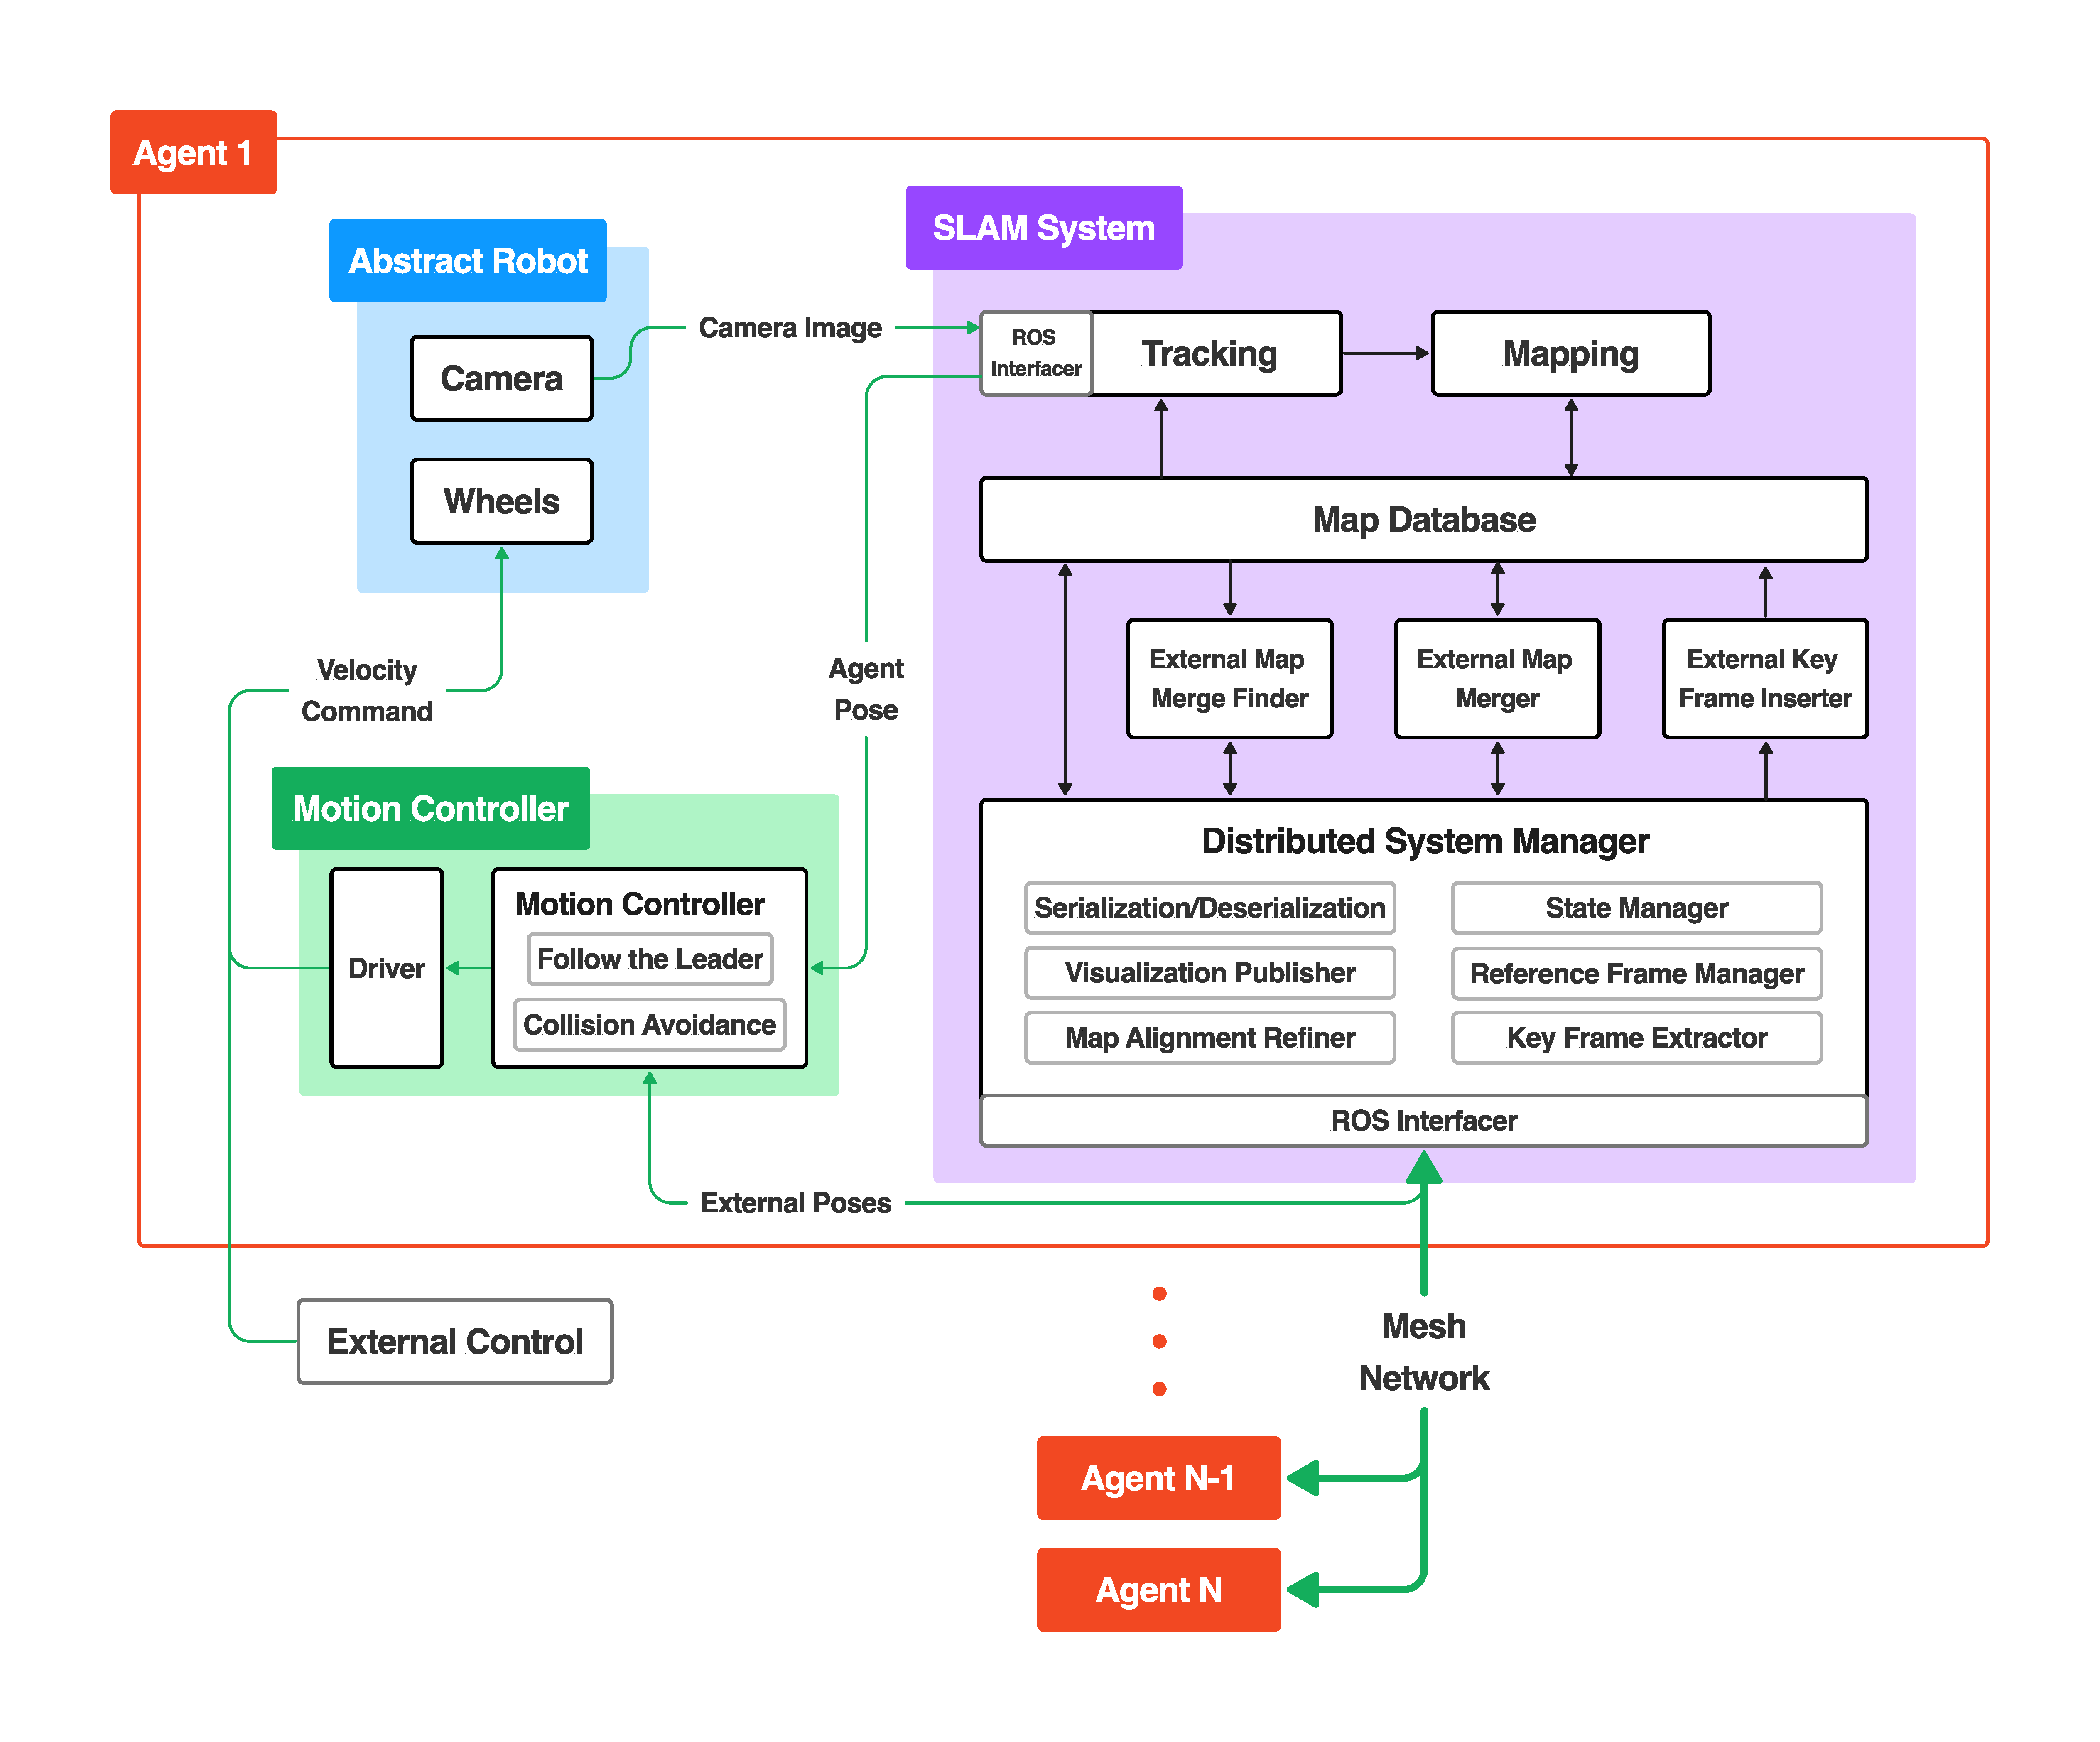
\includegraphics[trim=5cm 5cm 5cm 29cm, scale=0.2]{figures/agent_diagram.pdf}
    \caption{Agent diagram. Green arrows represent messages sent over ROS topics, while black arrows represent internal communications within a node.}
    \label{fig:agent-diagram}
\end{figure}

\autoref{fig:agent-diagram} gives an architectural overview of an agent in my system, showing how the \texttt{Abstract Robot}, \texttt{SLAM System} and \texttt{Motion Controller} ROS nodes interconnect.

From a high level, we have an \texttt{Abstract Robot} node that provides an interface to the robot's hardware. This sends camera images to the \texttt{SLAM System} node, which builds a map of the world in collaboration with its peers. The \texttt{Motion Controller} node receives agent pose information from both the local \texttt{SLAM System} and the external peers to perform tasks such as collision avoidance by sending velocity commands back to the \texttt{Abstract Robot} node, closing the control loop.

In the following sections, we will explore these nodes in detail.

\section{SLAM System}
\label{sec:slam-system}
The SLAM System node is the majority of this project's implementation. It processes monocular images from the camera to localize the agent while also collaboratively building up a map of the world with its peers. As discussed in \autoref{sec:starting-point}, my system is based on an existing single-agent SLAM system that performs the \texttt{Tracking} and \texttt{Mapping} tasks. While substantial modifications were made to the base single-agent system, I will generally focus on the decentralized aspects of the system in the interest of space.

\subsection{Data Structures}
\label{sec:datastructures}
A brief discussion of my SLAM system's internal data structures is required to understand the following sections. \autoref{fig:datastructure-diagram} shows the two key data structures: the map database and the visual word set. The map database contains multiple maps, which primarily consist of keyframes and map points. Keyframes are selected frames from the camera feed, containing the predicted pose of the agent at that time along with the observed world features which we call ``map points". These map points can be observed by multiple keyframes, as shown in \autoref{fig:datastructure-viz}, and when this happens we connect the keyframes with a ``co-visible" link.

Keyframes also have a ``visual bag of words" representation, which is the vector describing the visual contents of the keyframe. These are essential for detecting potential map merges, so we also build a ``visual word set" that allows us to find all keyframes that contain a particular visual word\footnote[1]{A ``visual word'' is a feature from the bag of words vocabulary.}.


\begin{figure}[h]
    \centering
    \begin{subfigure}[b]{0.475\textwidth}
        \centering
        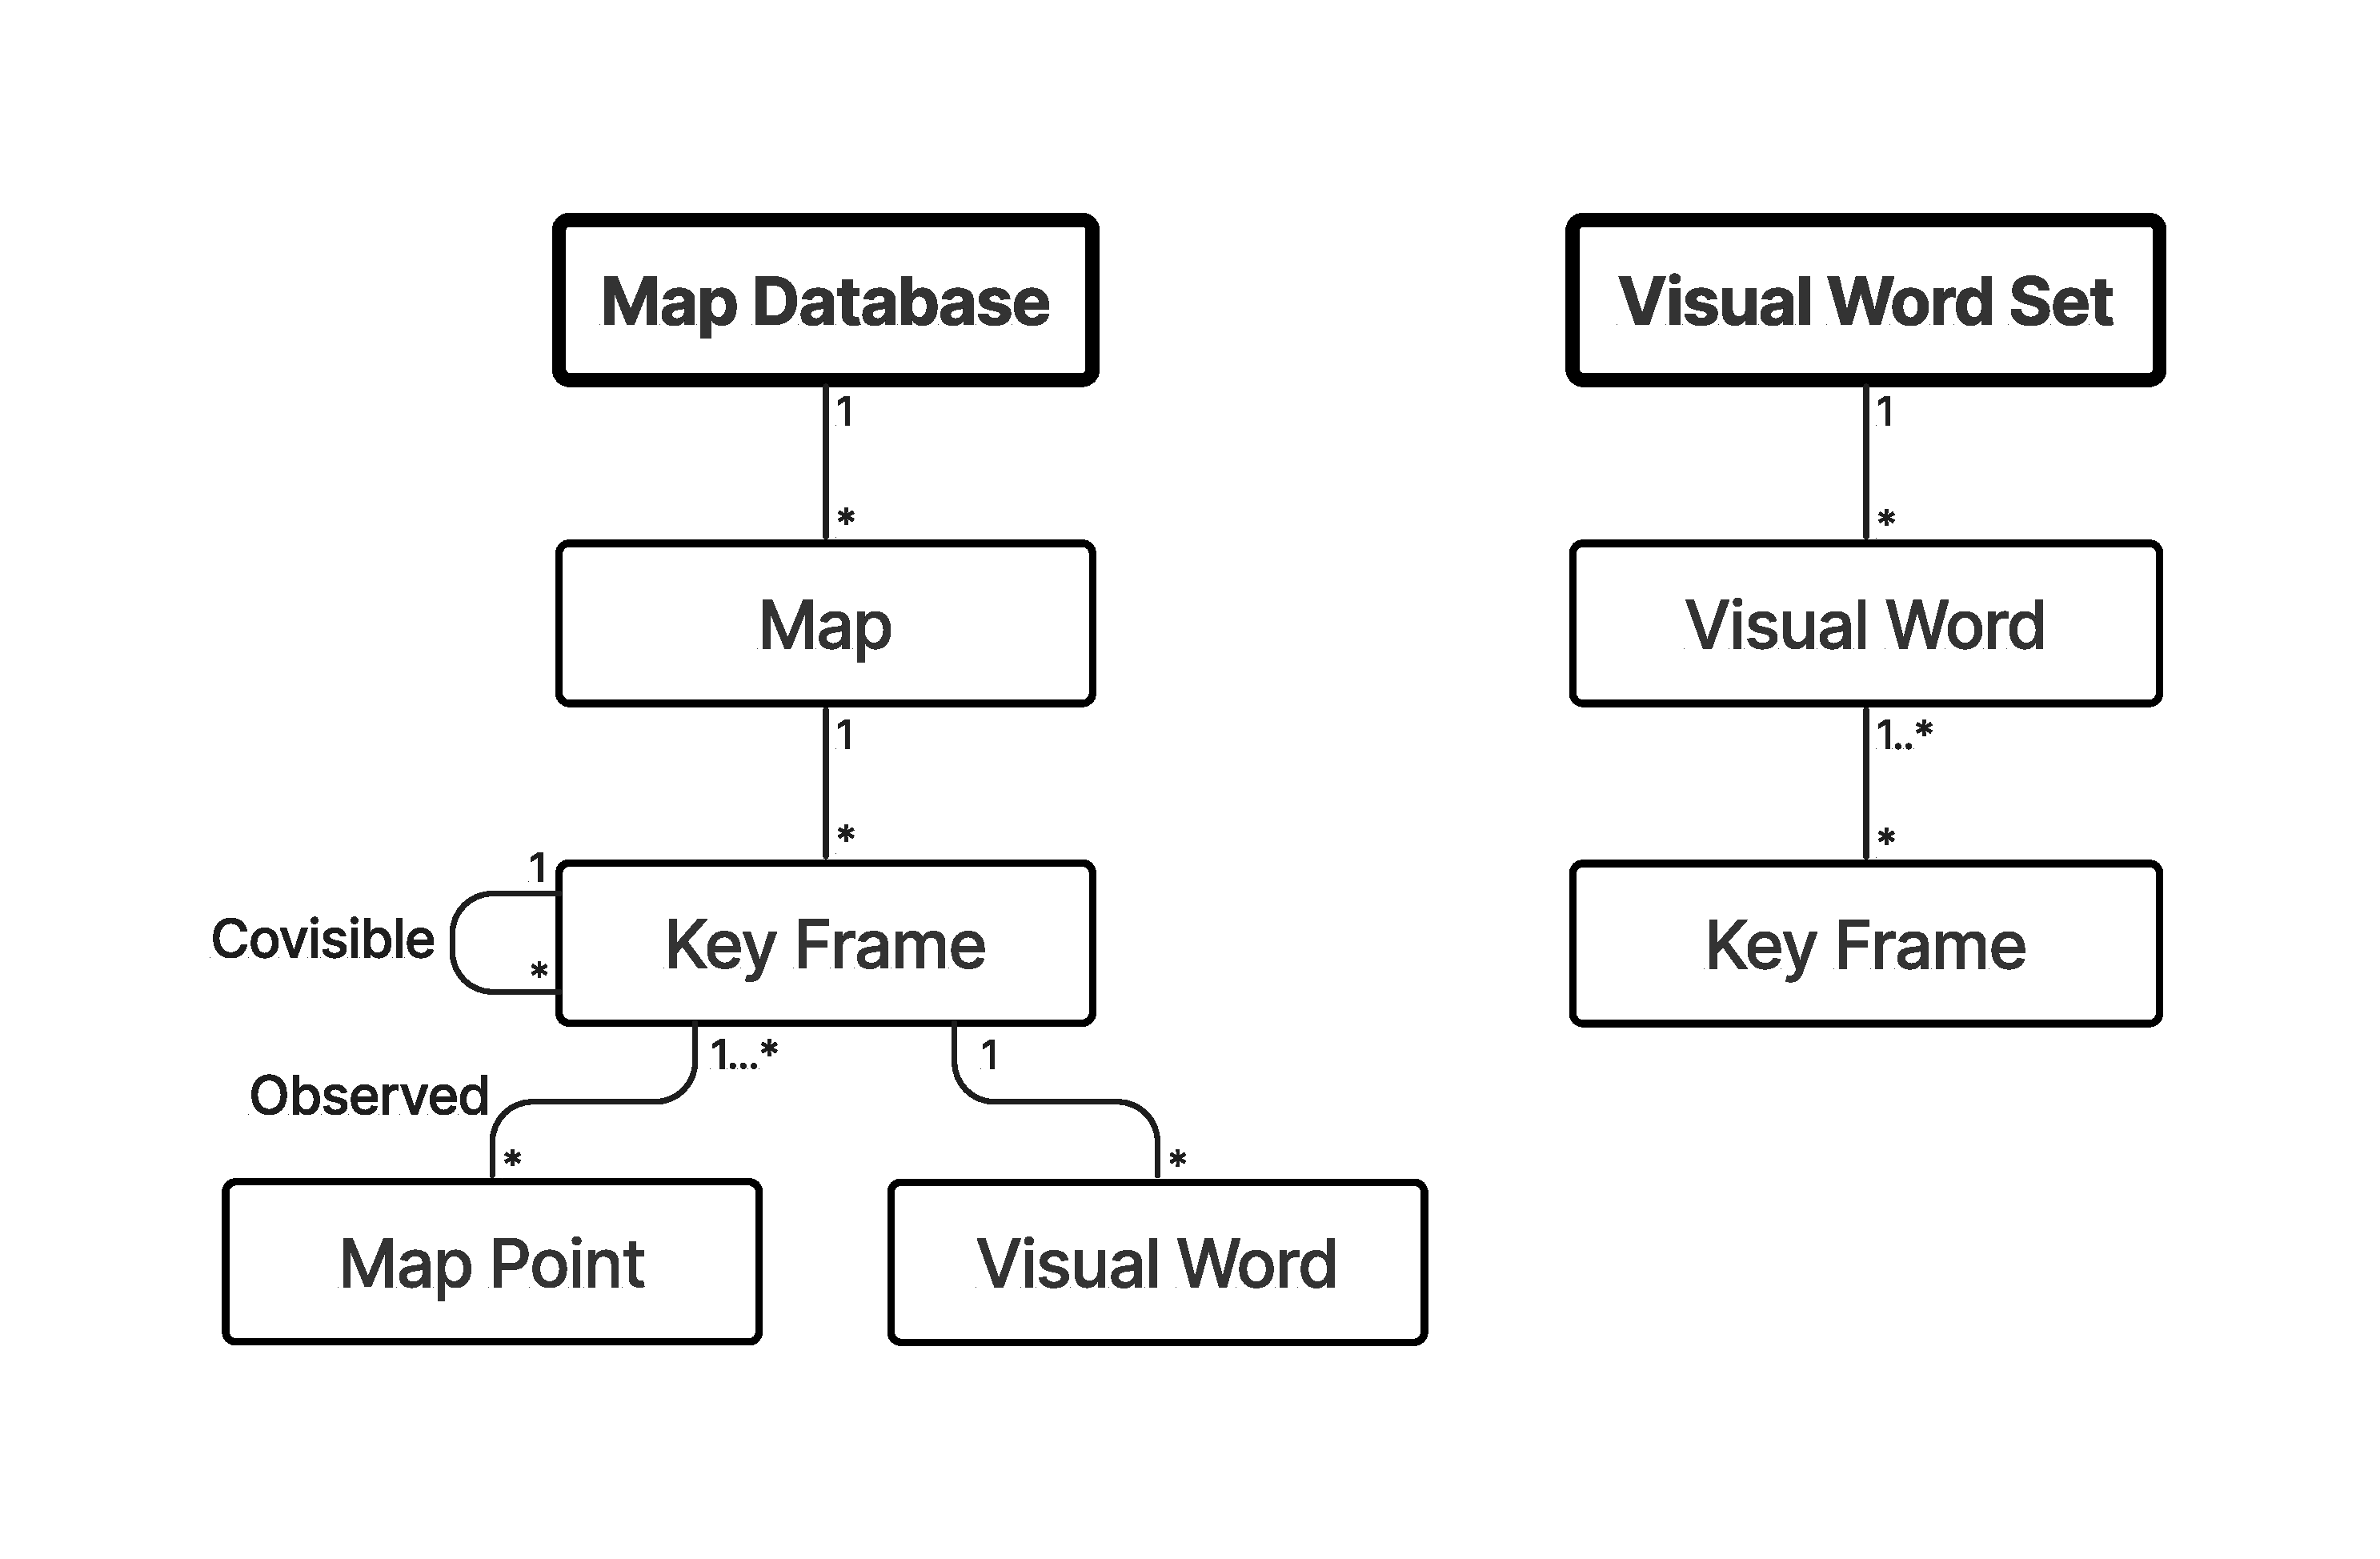
\includegraphics[trim=5cm 4cm 5cm 5cm, width=\textwidth]{figures/datastructure_diagram.pdf}
        \caption{Data structure diagram}
        \label{fig:datastructure-diagram}
    \end{subfigure}\hfill%
    ~
    \begin{subfigure}[b]{0.425\textwidth}
        \centering
        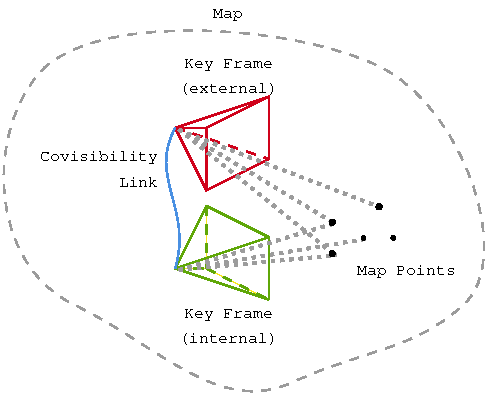
\includegraphics[width=\textwidth]{figures/datastructure_viz.pdf}
        \caption{Visual representation of data structure}
        \label{fig:datastructure-viz}
    \end{subfigure}%
\end{figure}

\subsection{Decentralized System Manager}
\label{sec:decentralized-system-manager}
Decentralized SLAM systems are significantly more complex than single-agent or even centralized systems, due to the nuanced interactions between agents as they merge maps, lose localization, or lose connection with their peers. Therefore, a robust framework must be put in place to ensure the correctness of the system, which I have implemented in the \texttt{Decentralized System Manager} component.

For the sake of simplicity, the next few sections will explore the interactions between just two agents: a \textit{local} and \textit{external} agent. In the \nameref{sec:generalizing-to-n-geq-3-agent-systems} section, we will show how this easily generalizes to a system with an arbitrary number of agents.

\subsection{State Manager}
\label{sec:state-manager}

\begin{figure}[h]
    \centering
    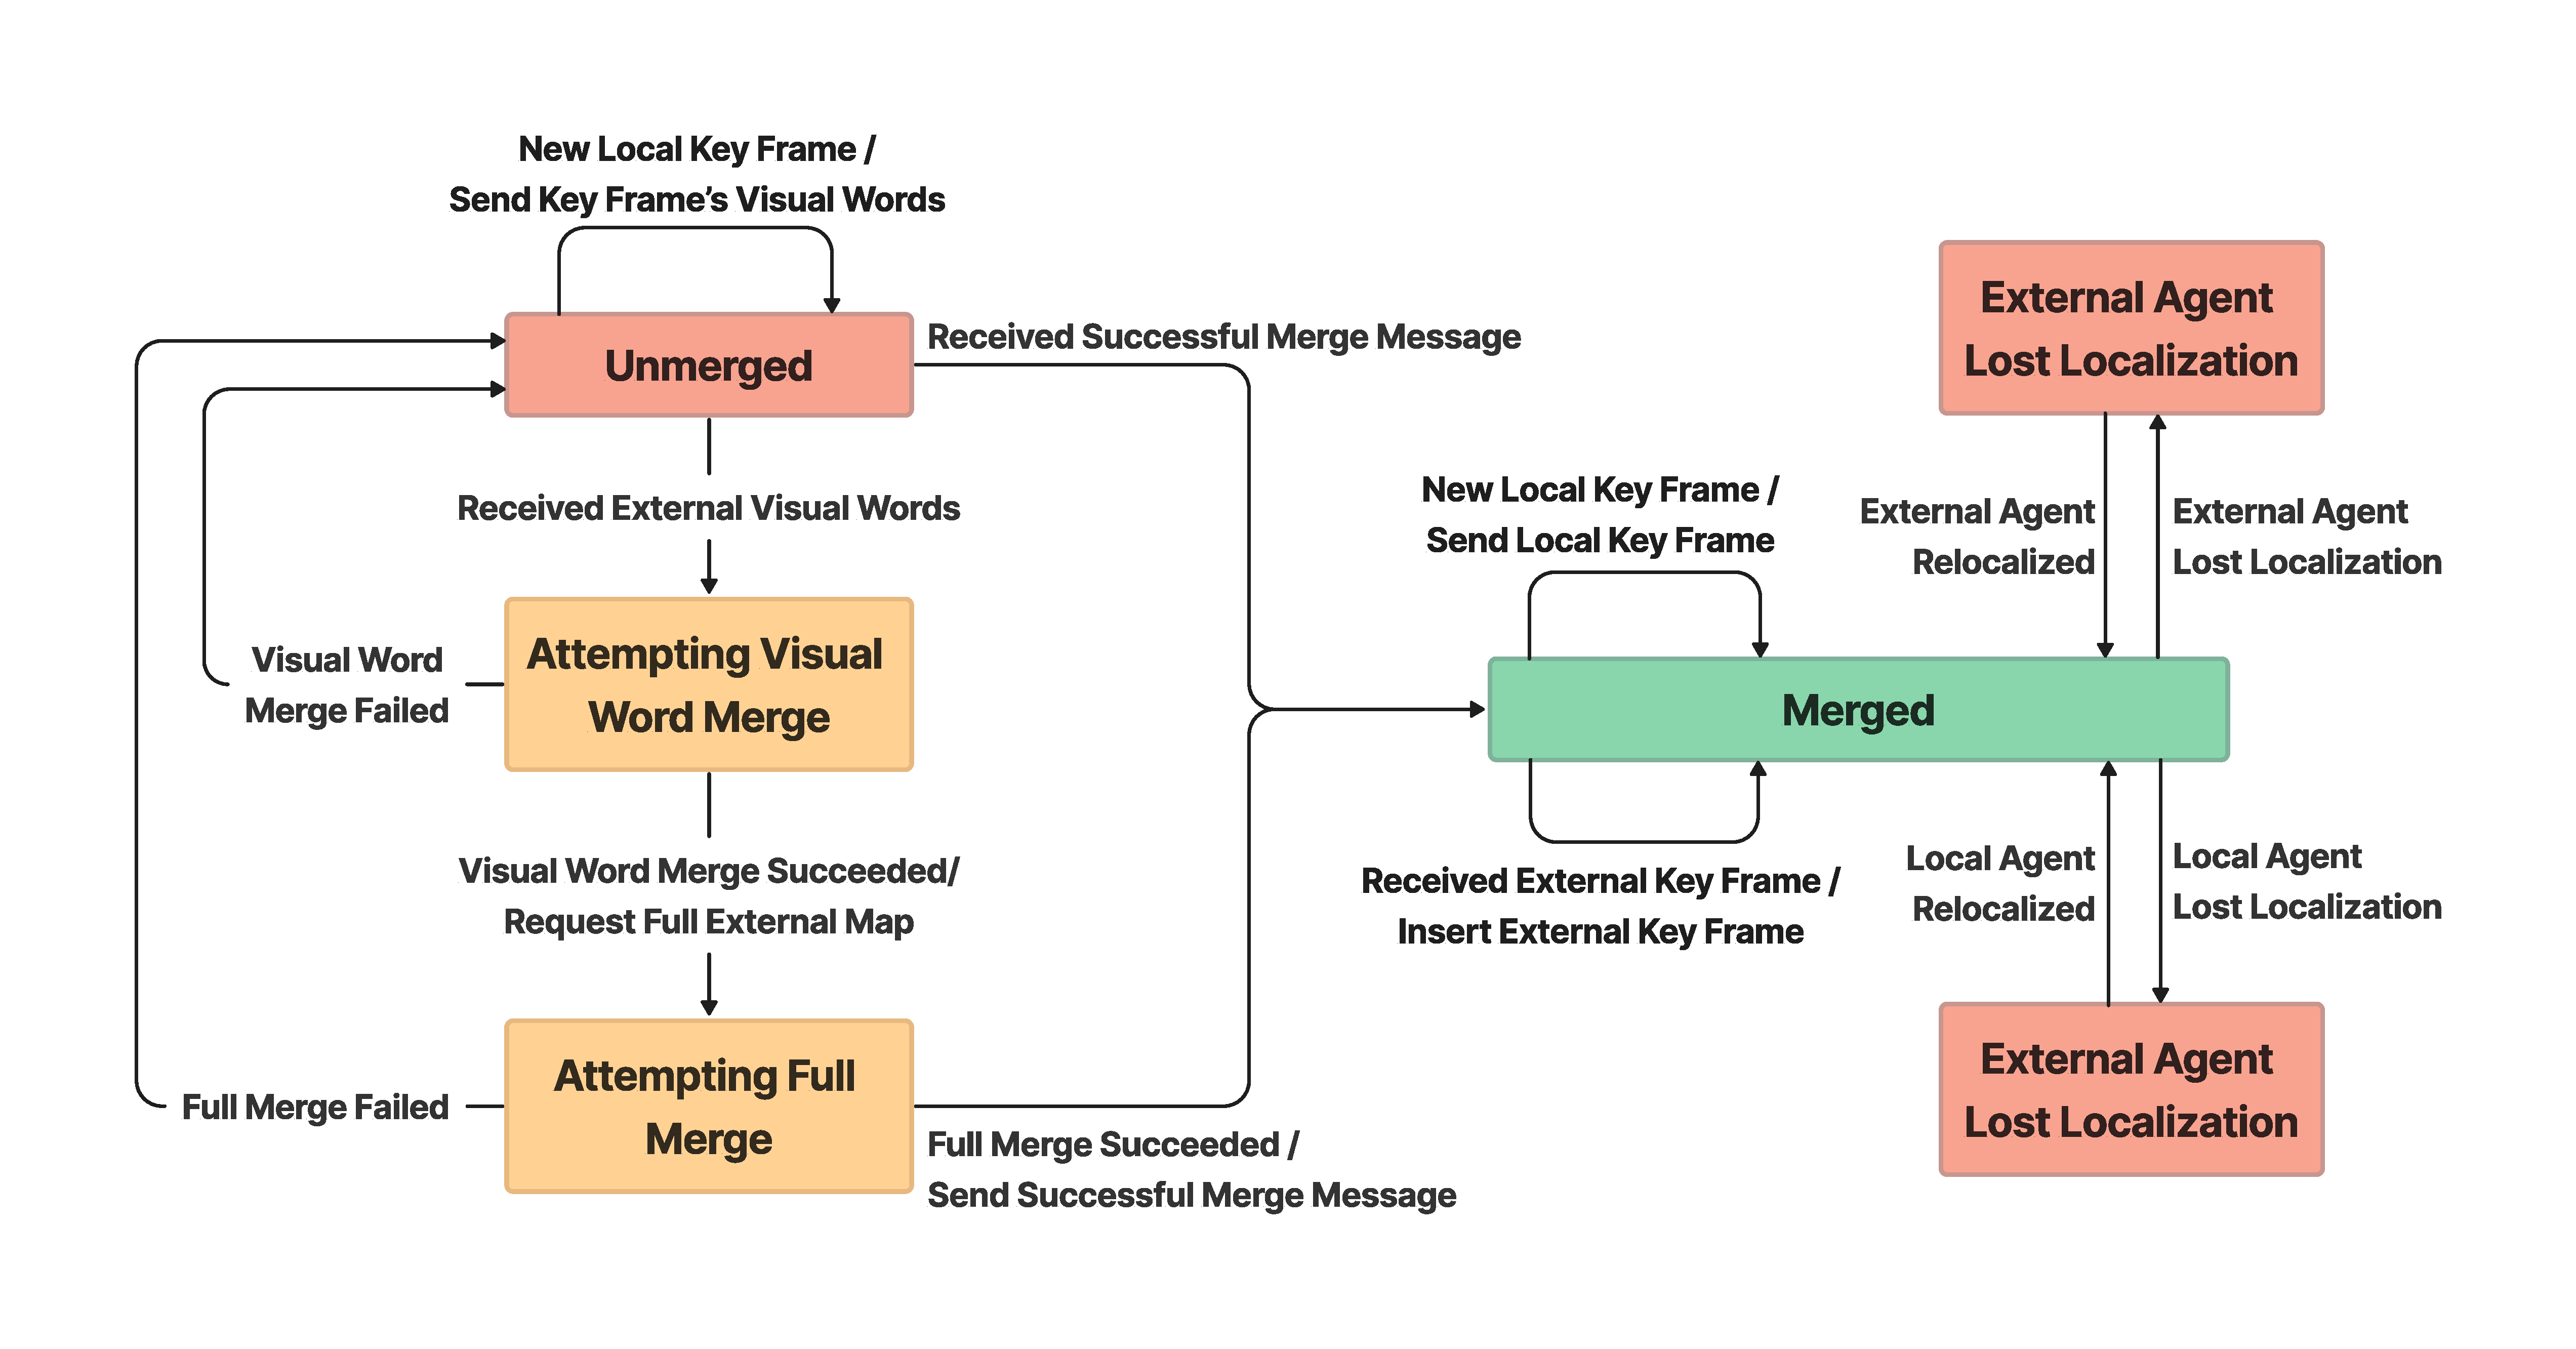
\includegraphics[trim=5cm 5cm 5cm 5cm, width=\linewidth]{figures/slam_system_state_machine.pdf}
    \caption{SLAM system state machine for a single peer. Mealy machine notation is used, where each transition is defined as: \texttt{input}/\texttt{output}.}
    \label{fig:state-machine}
\end{figure}

Each agent's \texttt{Decentralized System Manager} maintains a state machine for every peer in the system, shown in \autoref{fig:state-machine}. All peers are initialized in the \texttt{unmerged} state, meaning that they are in different coordinate frames and share a unified map. As the local agent starts to explore the same locations as its peers, the system recognizes the visual overlaps and merges their maps, bringing us to the \texttt{merged} state where the agents share the same coordinate frame and map, enabling relative positioning and collaborative map building.


\subsection{Map Serialization and Deserialization}
\label{sec:map-serialization-and-deserialization}
Map serialization and deserialization are essential and non-trivial components of this SLAM system, enabling agents to share their maps across the network. For this task, I used the Boost Serialization C++ library \autocite{boostLibrary} since it supports standard library collections and other common classes.

As discussed in \autoref{sec:datastructures}, maps contain keyframes and map points. Individually, these objects are relatively easy to serialize with boost – in fact, the single agent SLAM program my system is based on already supported saving and loading maps allowing me to leverage some of their serialization helper functions. To serialize these objects we simply need to define a serialization scheme for each class, describing which instance variables should be serialized and which shouldn't.

% Strategically selecting only the parameters that need to be serialized allows us to cut back on communication overhead. For example, there is no need for us to serialize a keyframe's raw image, as it is not used in the rest of our SLAM pipeline.

Complexities arise when we try to serialize/deserialize the connections between these objects, especially when we are only sending map fragments as we may be required to ``relink'' deserialized objects with objects in our local map. We manage these connections by giving every keyframe and map point a universal unique identifier (UUID), allowing us to use these UUIDs as references to a specific object in our multi-agent system. We use UUIDs since they do not require a centralized server or any communication with our peers to assign a unique ID to every object\footnote[1]{While not \textit{verifiablly} unique, UUIDs are unique within practical limits. A commonly cited anecdote is that it is far more likely for a cosmic ray to cause a bug than a UUID collision.}.

% For example, if we send a new keyframe $k$ and its map points $M_k$ to an external agent, due to the many-to-many relationship between keyframes and map points, some of the map points in $M_k$ may have already been sent before. We can define $M_k = M_{k\_sent} \cup M_{k\_unsent}$, where $M_{k\_sent}$ are the map points that have already been sent to the external agent and $M_{k\_unsent}$ are the ones that have not. Map points in $M_{k\_sent}$ will need to be connected to $k$ when it is deserialized by the external agent, and map points in $M_{k\_unsent}$ will need to be sent to the external agent and connected to any existing keyframes in the external map that observe the map points. These connections are further explained in the \nameref{sec:external-key-frame-inserter} section, particularly \autoref{fig:external-keyframe-inserter}.

This method of using UUIDs as references is used to rebuild all connections after deserialization, including the keyframe-to-keyframe connections that build the co-visibility graph and many others that I have not had the space to discuss in this dissertation. A good example of connection rebuilding is later given in \autoref{fig:external-keyframe-inserter}, which shows how external map fragments are relinked with the local map.

\subsection{External Map Merge Finder}
\label{sec:external-map-merge-finder}
A naive approach to merging our map with an external agent is to constantly exchange our full maps, each time trying to identify if a map merge is possible. While simple, this approach does not scale well from both a networking and computational perspective, as maps are often $\geq$1MB in size, and computing a full map merge is extremely computationally expensive.

Instead, we first identify if a map merge is even feasible by using visual words. This eliminates superfluous map merge attempts that have no chance of succeeding because the agents' maps have no visual overlap.

As an agent generates new keyframes, we use DBoW2 \autocite{GalvezTRO12} to calculate the \hyperref[sec:visual-bag-of-words]{visual bag of words} seen by the keyframe and send them to our peers. These visual words are significantly smaller than sending over the complete keyframe (as shown in \autoref{fig:kf-vs-bow-msg-size}) and enable agents to detect if there is a significant amount of visual overlap between its local map and the external agent's map.

\autoref{alg:map-merge-finder} is used to calculate if a merge is found by comparing the merge score of the external visual words to a dynamic baseline merge score, allowing the system to generalize to different environments. \autoref{alg:calculate-merge-score} is the subprocedure used to calculate this merge score metric, giving a numerical value representing how well a visual bag of words ``fits'' into the local map. Notably, the algorithm exploits the spatial locality of keyframes which was found to give a more robust score.

This method gives a recall of almost 100\%, at the cost of potentially lower precision. This is a worthwhile tradeoff, however, as it is essential to have very few false negatives so we can merge maps as soon as possible and the agents can begin collaborating.

\begin{figure}[h]
    \centering
    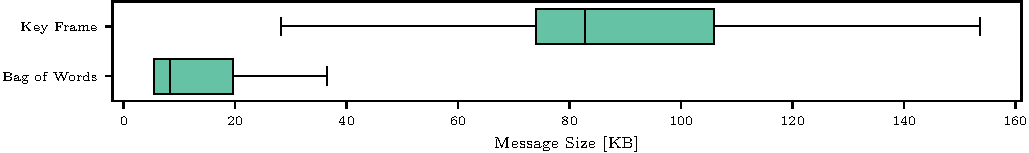
\includegraphics[width=\linewidth]{figures/apr20_mh_trajectory_g_kf_vs_bow_msg_size.pdf}
    \caption{Comparison of the message size difference between a raw keyframe and a bag of words representation of a keyframe.}
    \label{fig:kf-vs-bow-msg-size}
\end{figure}
\hspace{0.15in}
\begin{algorithm}[H]
    \caption{Map merge finder using visual words.}
    \label{alg:map-merge-finder}
    \begin{algorithmic}[1]
        \Require{VisualWords$_{ext}$: Set containing external keyframe's visual words}
        \Ensure{Success: Boolean value signaling if a merge is possible based on visual words}
        \State (MergeScore$_{ext}$, BestMatchKeyFrame) $\gets$ \textsc{CalculateMergeScore}(VisualWords$_{ext}$)
        \State (MergeScore$_{baseline}$, $\underbar{\ \ }$) $\gets$ \textsc{CalculateMergeScore}(BestMatchKeyFrame's visual words)
        \State Success $\gets$ MergeScore$_{ext}$ $\geq$ 0.7 $\times$ MergeScore$_{baseline}$
    \end{algorithmic}
\end{algorithm}
\vspace{-0.25in}
\begin{algorithm}[H]
    \caption{Calculate how well a bag of visual words merges with the local map.}
    \label{alg:calculate-merge-score}
    \begin{algorithmic}[1]
        \Procedure{CalculateMergeScore}{VisualWords}
        \State PotentialMatches $\gets$ query Visual Word Set data structure for similar keyframes
        \State BestMatchKeyFrame $\gets$ null
        \State BestMergeScore $\gets$ 0
        \For{each KeyFrame$_0$ in PotentialMatches}
        \State MergeScore $\gets$ KeyFrame$_0$'s similarity to VisualWords
        \State Covisible $\gets$ 5 keyframes with highest covisibility with KeyFrame$_0$
        \For{each KeyFrame$_{cov}$ in Covisible} \Comment{\textit{Exploit spatial locality}}
        \State MergeScore += KeyFrame$_{cov}$'s similarity to VisualWords
        \EndFor
        \If{MergeScore $\geq$ BestMergeScore}
        \State BestMergeScore $\gets$ MergeScore
        \State BestMatchKeyFrame $\gets$ KeyFrame$_0$
        \EndIf
        \EndFor
        \Return (BestMergeScore, BestMatchKeyFrame)
        \EndProcedure
    \end{algorithmic}
\end{algorithm}

\subsection{External Map Merger}
\label{sec:external-map-merger}
Once a potential map merge is found using visual words as described in the previous section, the external agent will send the local agent its full map and the local agent will attempt a full map merge using all the data.

Performing full map merges is perhaps the most important component of the decentralized SLAM system, as a bad map merge will make it impossible for agents to collaborate. Additionally, it is one of the most computationally intensive parts of this system, therefore, it has gone through numerous iterations to optimize performance and reduce map merge errors.


\begin{figure}[h]
    \centering
    \newcommand{\setheight}{1.25in}
    % \begin{subfigure}[t]{0.25\linewidth}
    %     \centering
    %     \raisebox{\dimexpr\setheight-.5\height}{%
    %         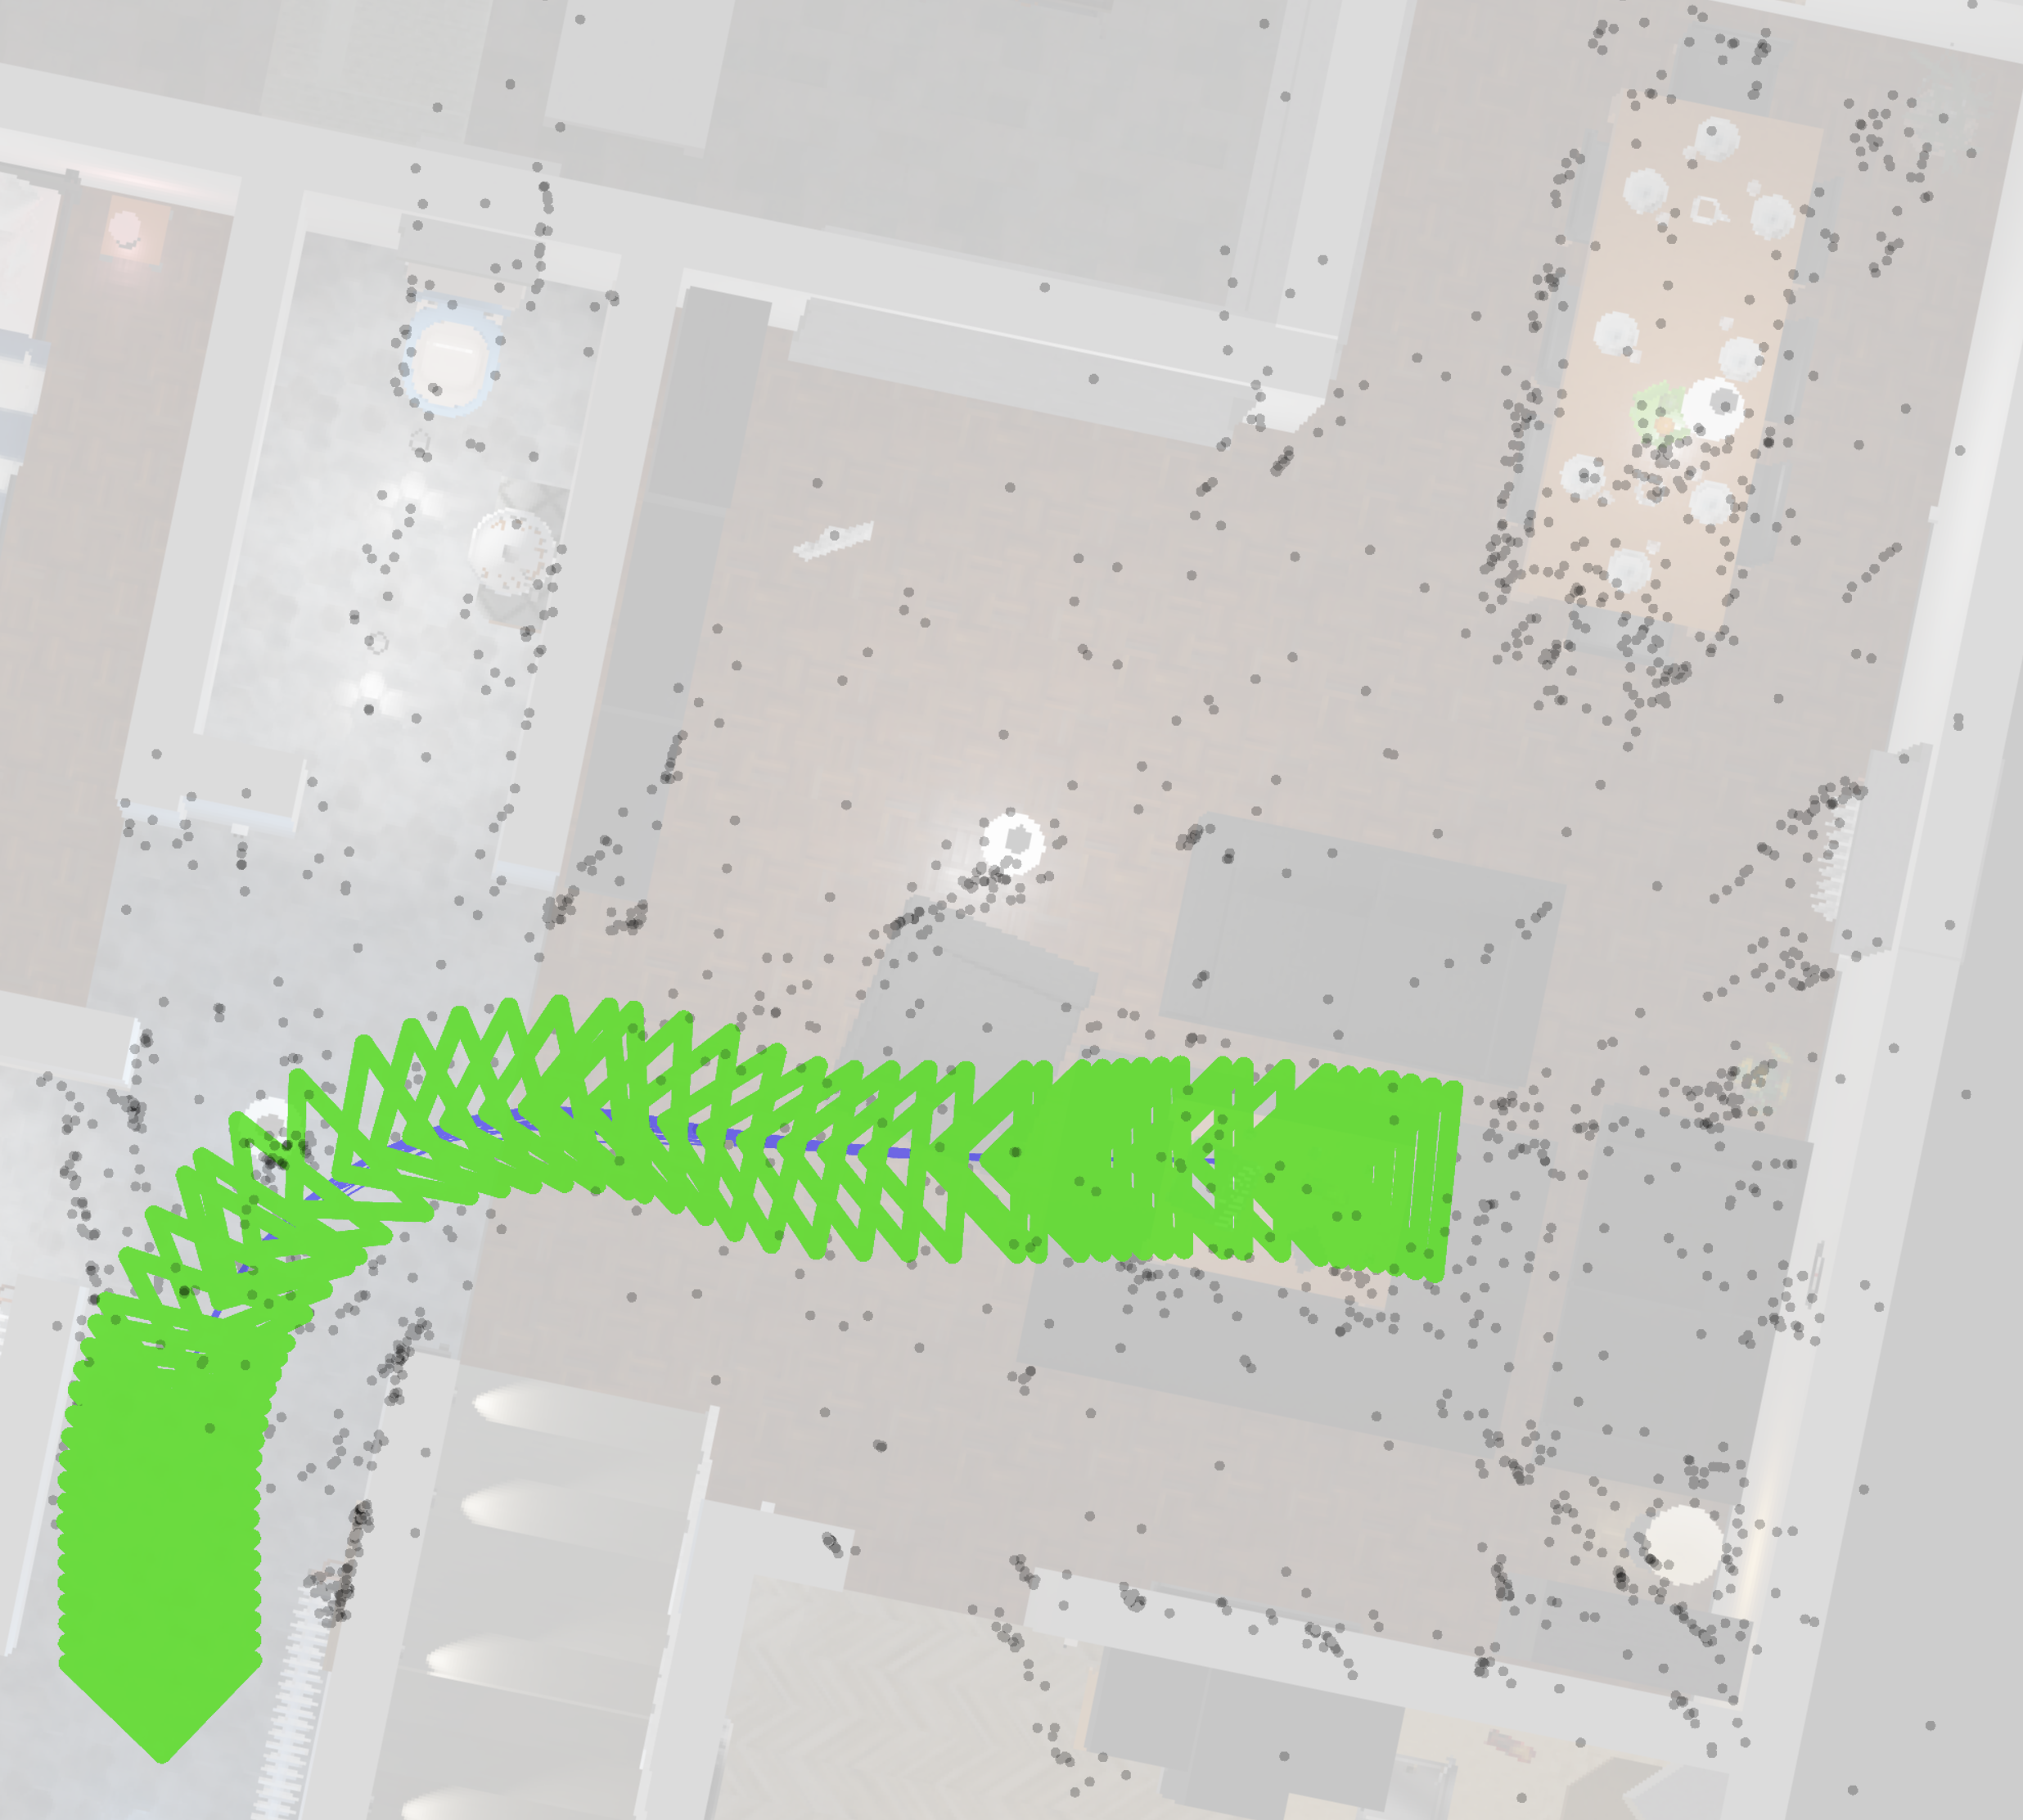
\includegraphics[width=\linewidth]{figures/pre_merge_1_w_floorplan.png}
    %     }
    %     \caption{Local map}
    % \end{subfigure}%
    % ~
    % \begin{subfigure}[t]{0.35\linewidth}
    %     \centering
    %     \raisebox{\dimexpr\setheight-.5\height}{%
    %         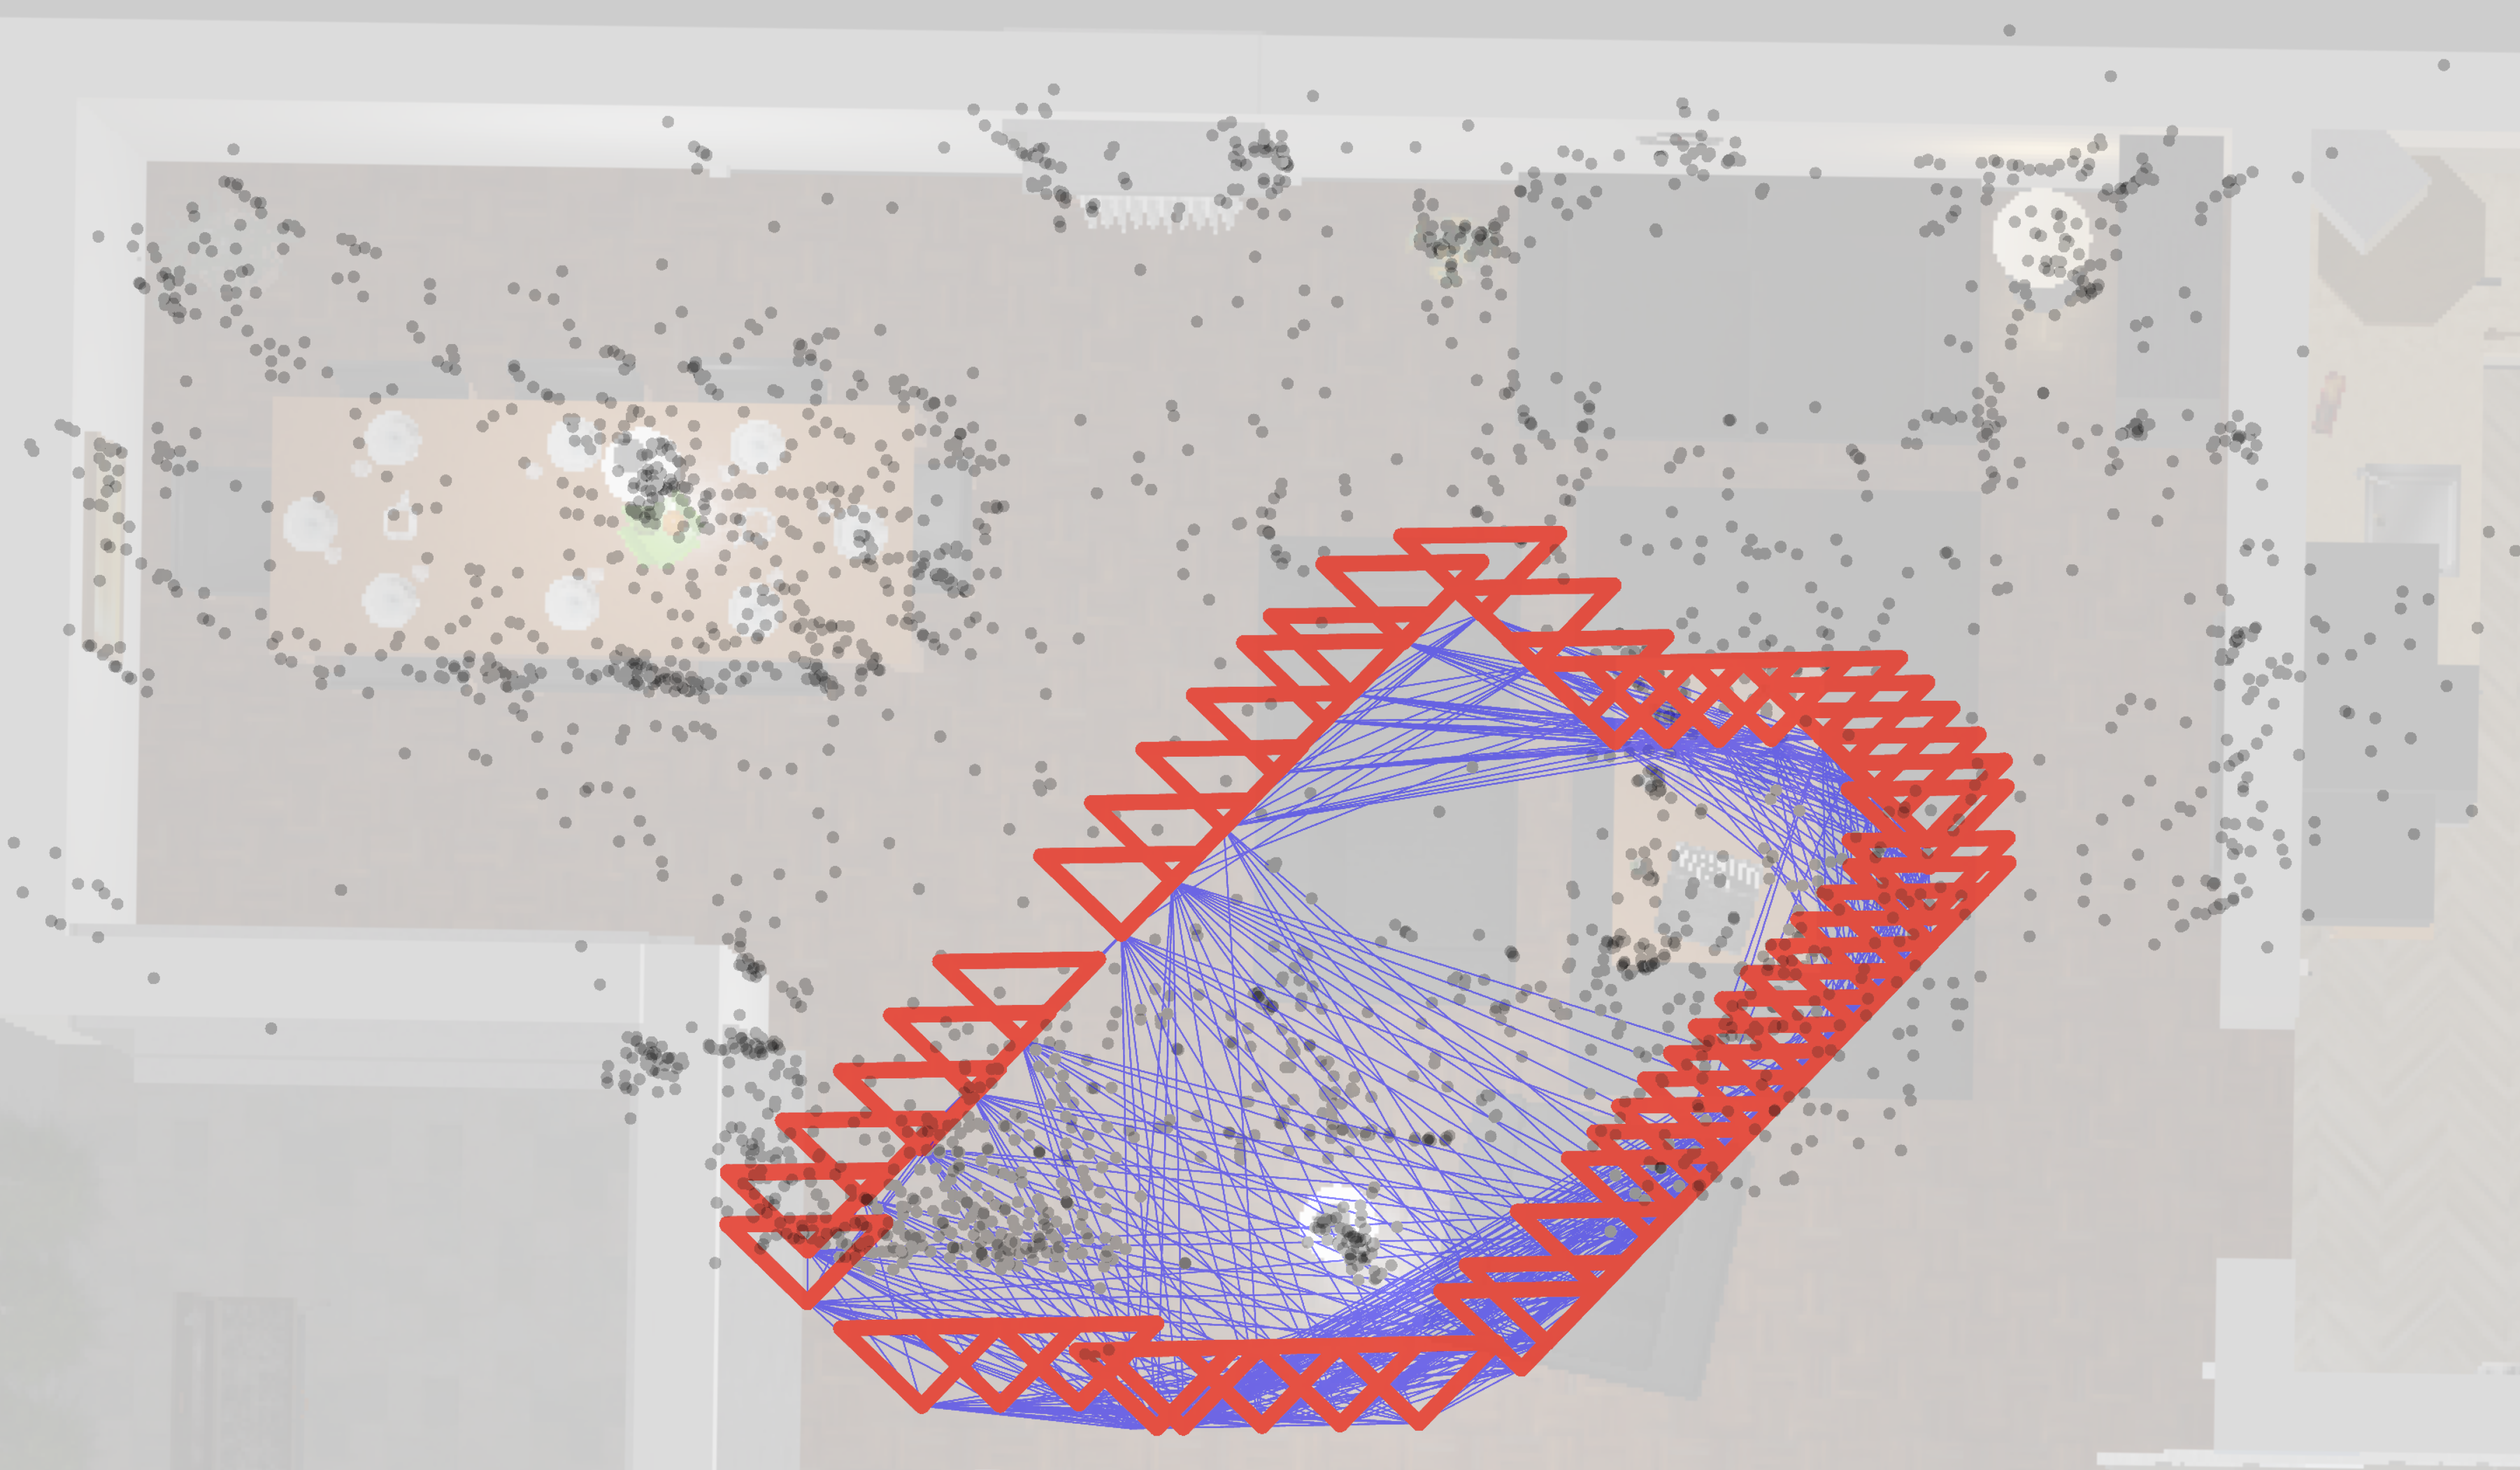
\includegraphics[width=\linewidth]{figures/pre_merge_2_w_floorplan.png}
    %     }
    %     \caption{External map}
    % \end{subfigure}%
    % ~
    % \begin{subfigure}[t]{0.4\linewidth}
    %     \centering
    %     \raisebox{\dimexpr\setheight-.5\height}{%
    %         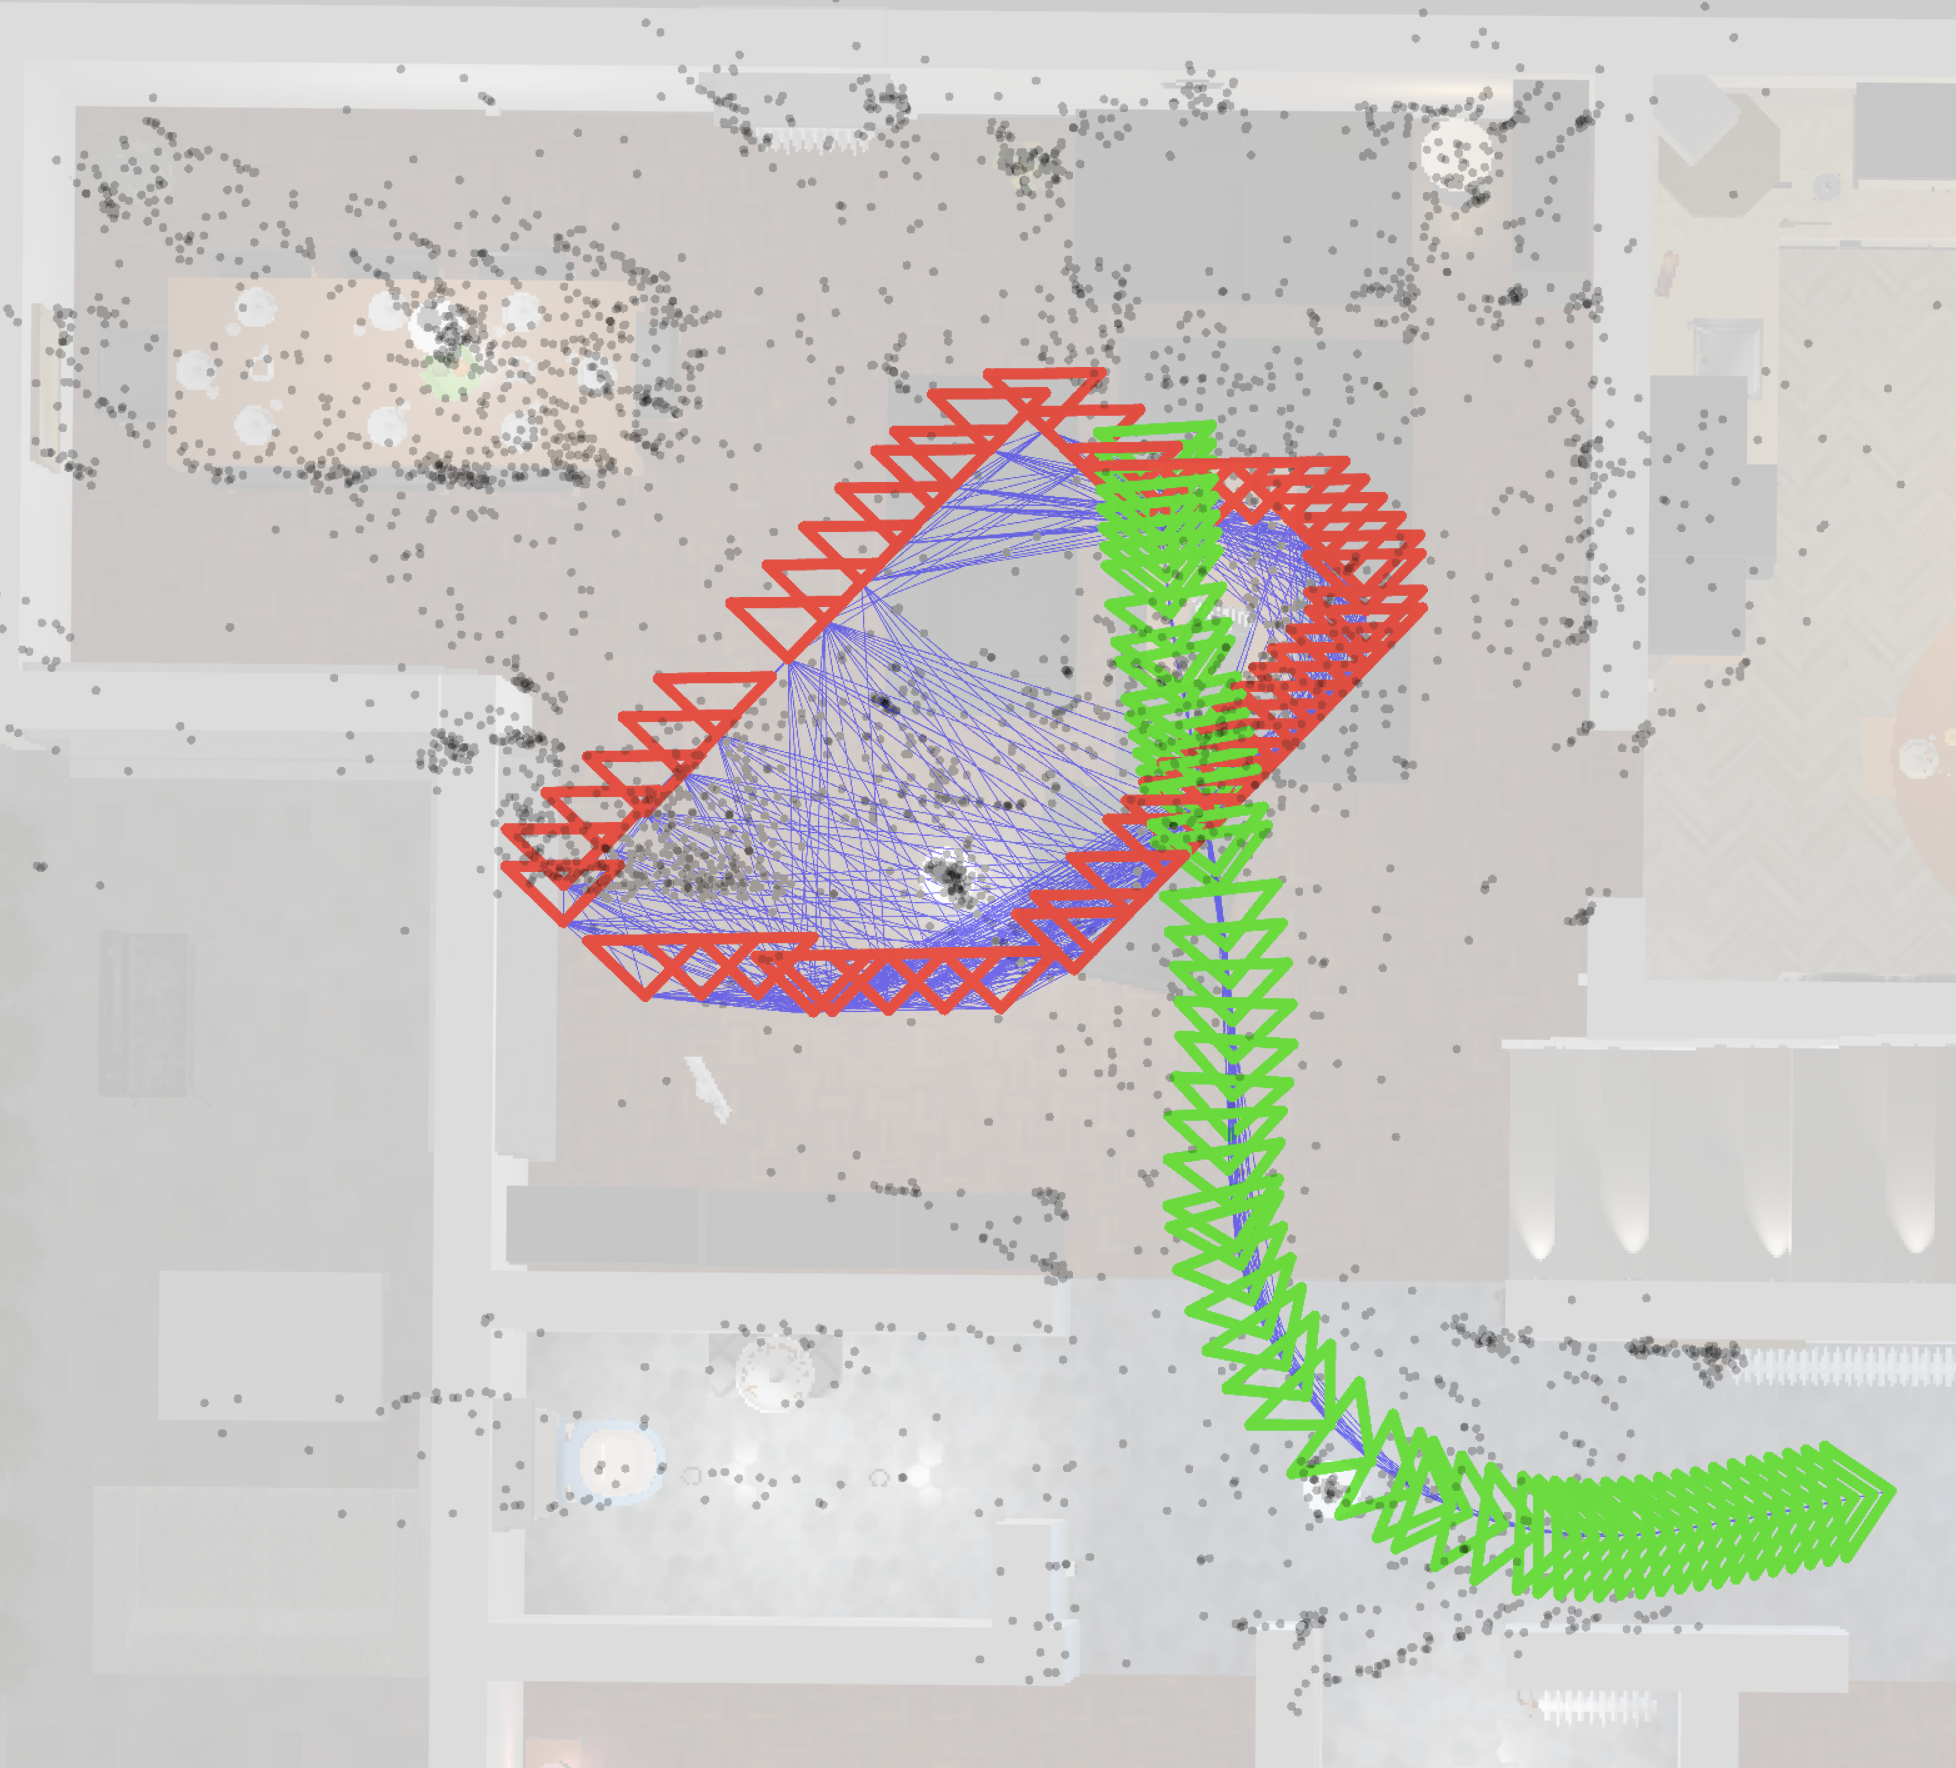
\includegraphics[width=\linewidth]{figures/after_merge_w_floorplan.png}
    %     }
    %     \caption{Merged map}
    % \end{subfigure}
    \begin{subfigure}[t]{0.25\linewidth}
        \centering
        \raisebox{\dimexpr\setheight-.5\height}{%
            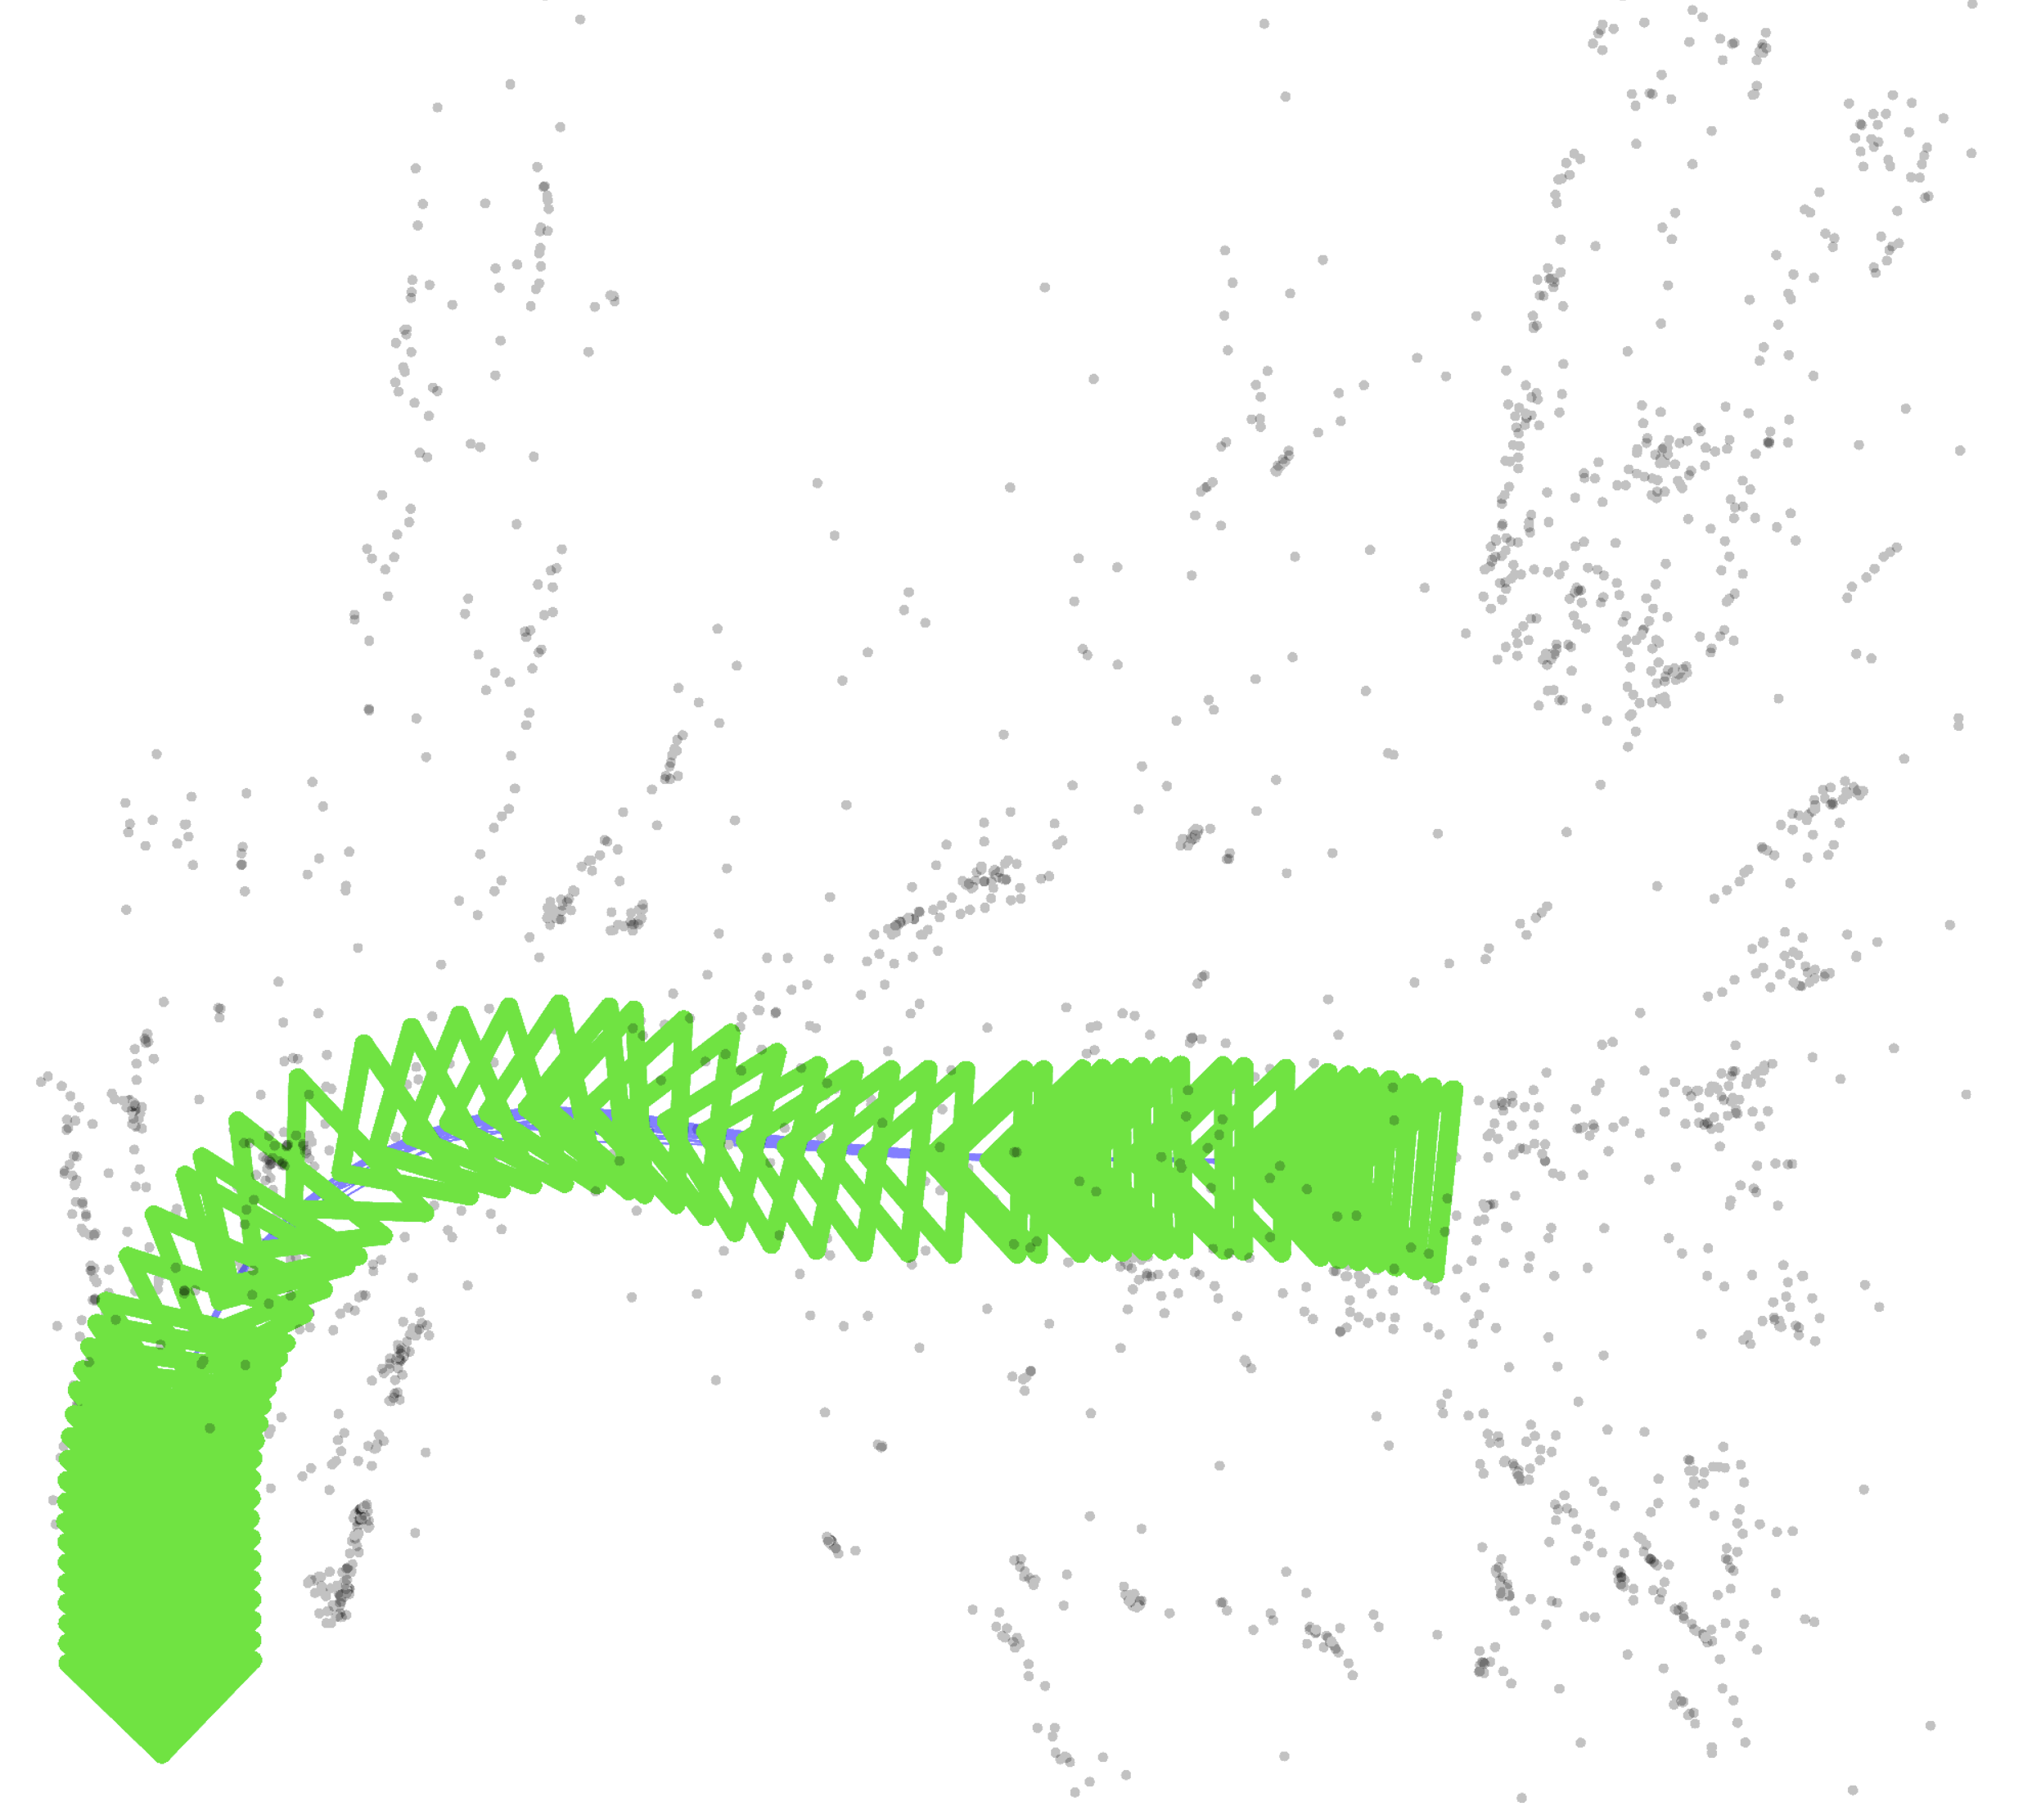
\includegraphics[width=\linewidth]{figures/pre_merge_1.png}
        }
        \caption{Local map}
    \end{subfigure}%
    ~
    \begin{subfigure}[t]{0.35\linewidth}
        \centering
        \raisebox{\dimexpr\setheight-.5\height}{%
            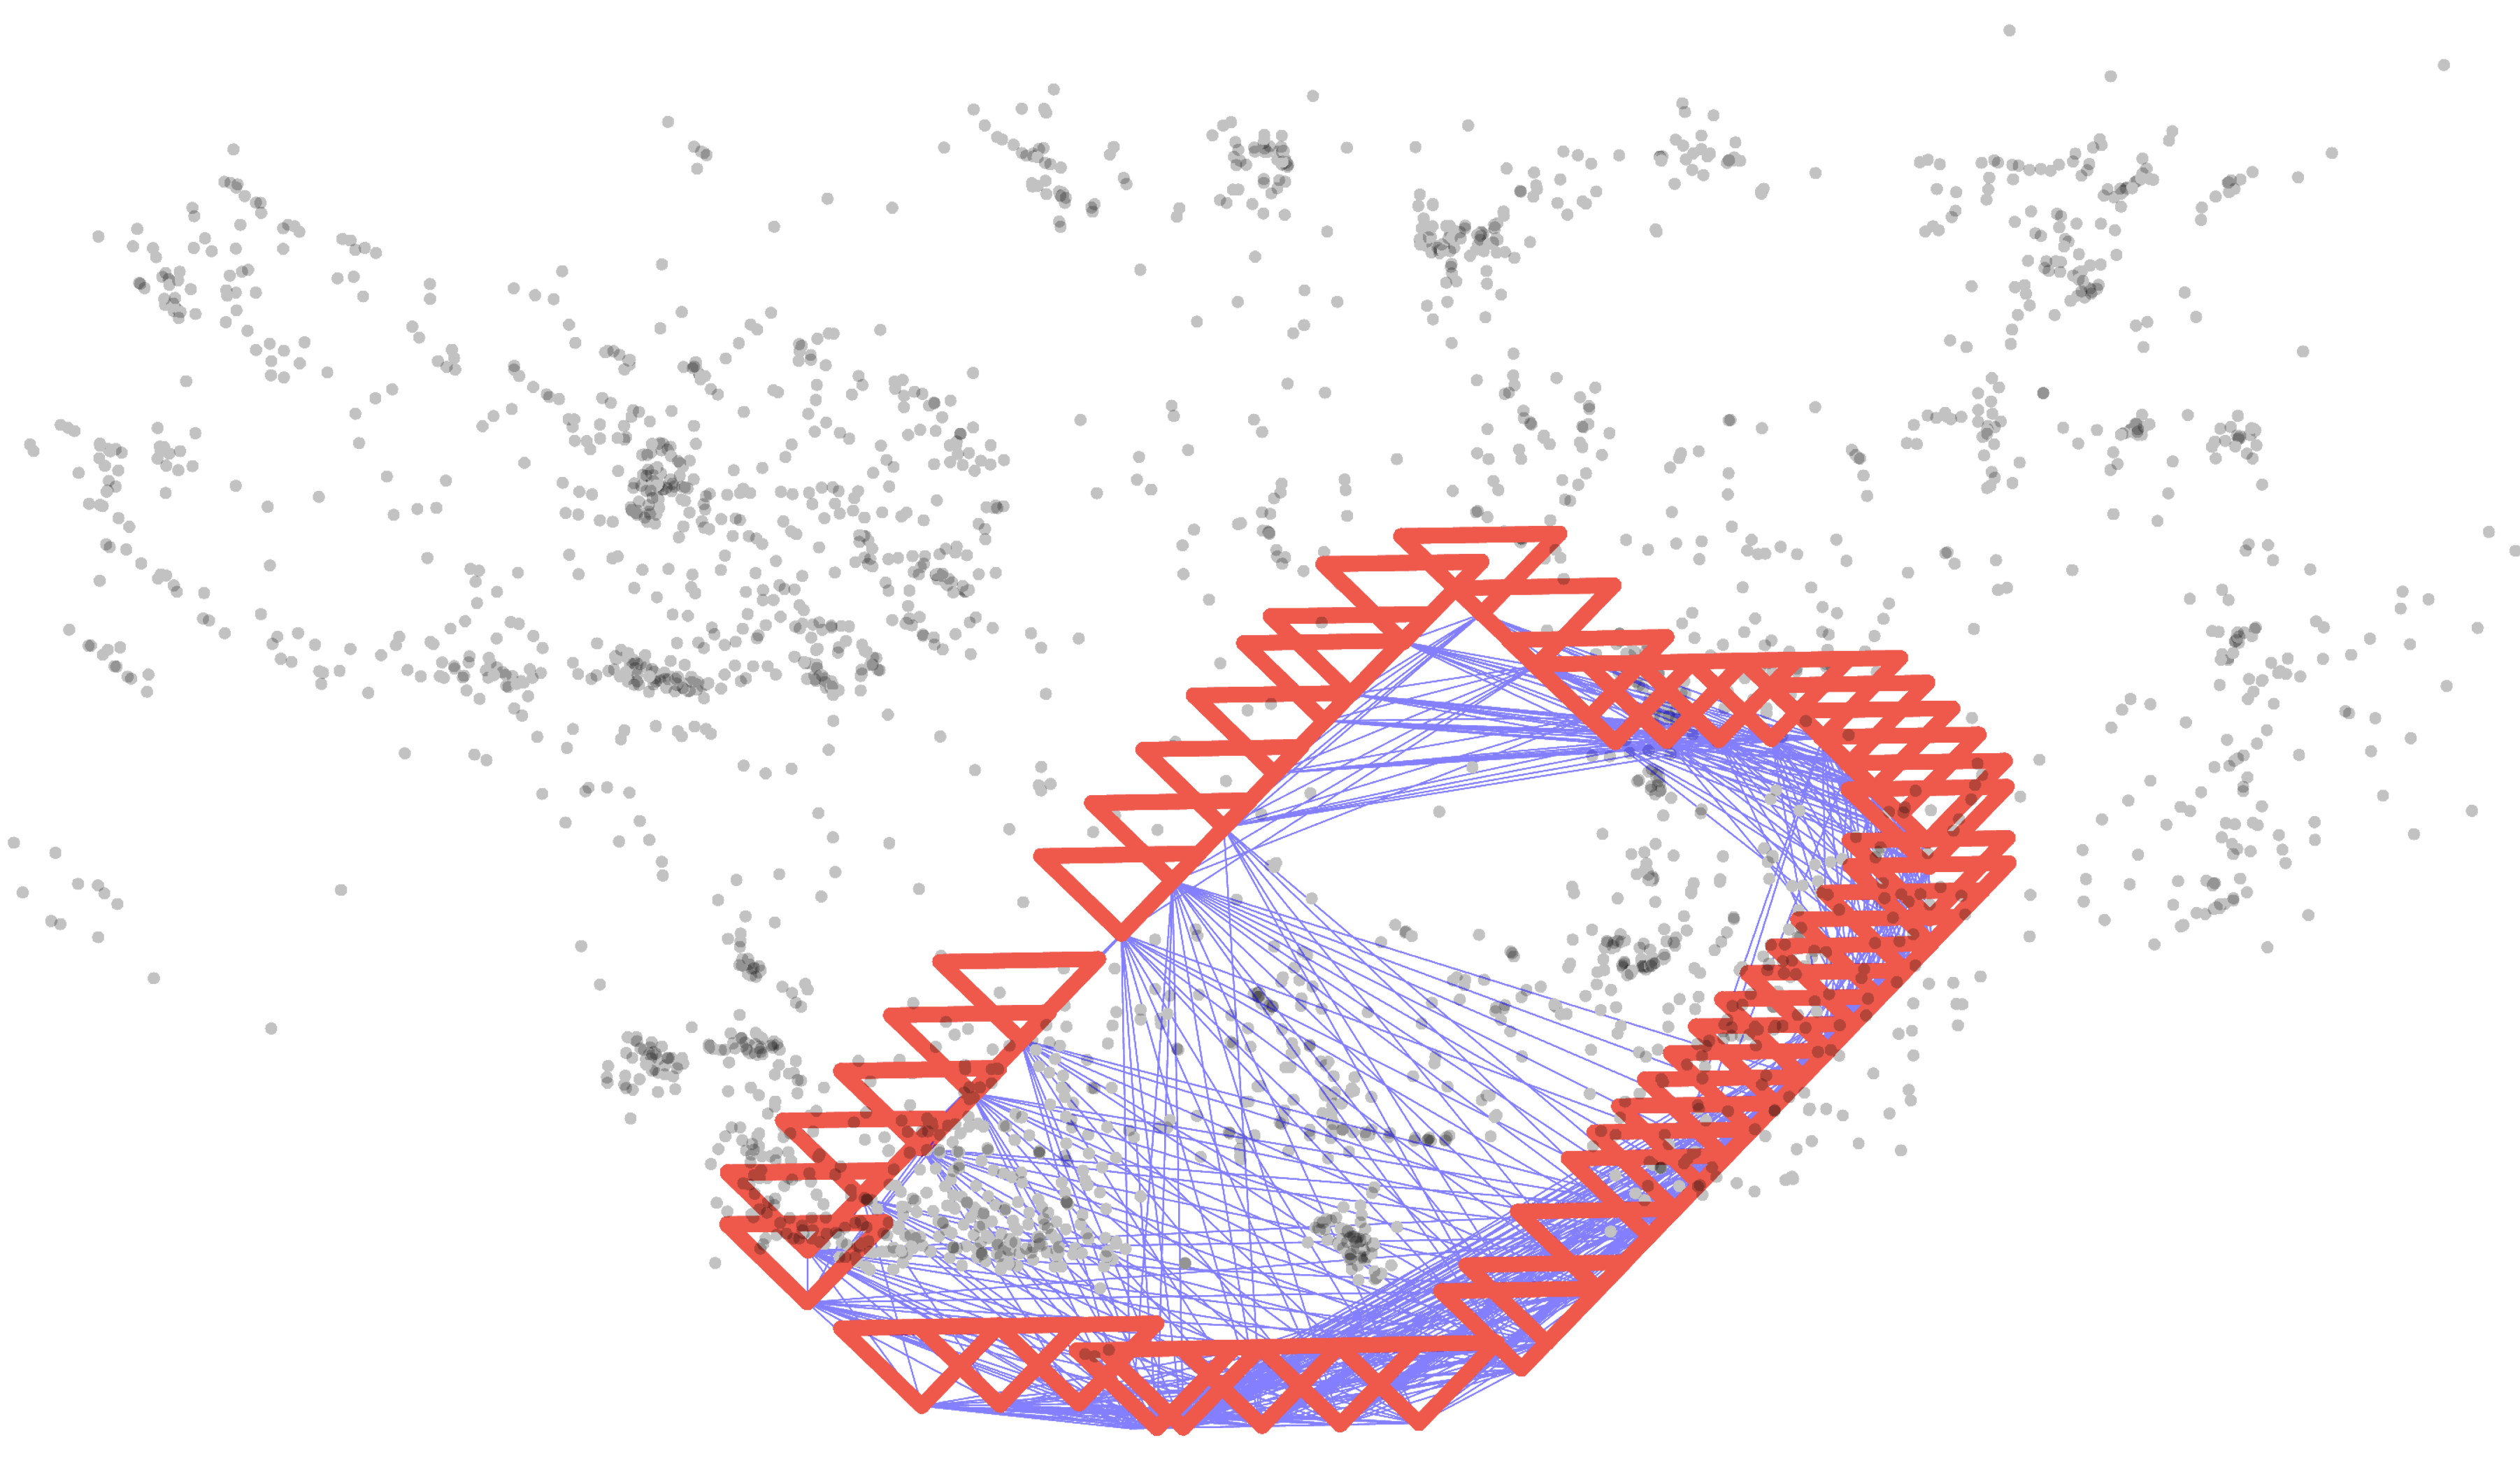
\includegraphics[width=\linewidth]{figures/pre_merge_2.png}
        }
        \caption{External map}
    \end{subfigure}%
    ~
    \begin{subfigure}[t]{0.4\linewidth}
        \centering
        \raisebox{\dimexpr\setheight-.5\height}{%
            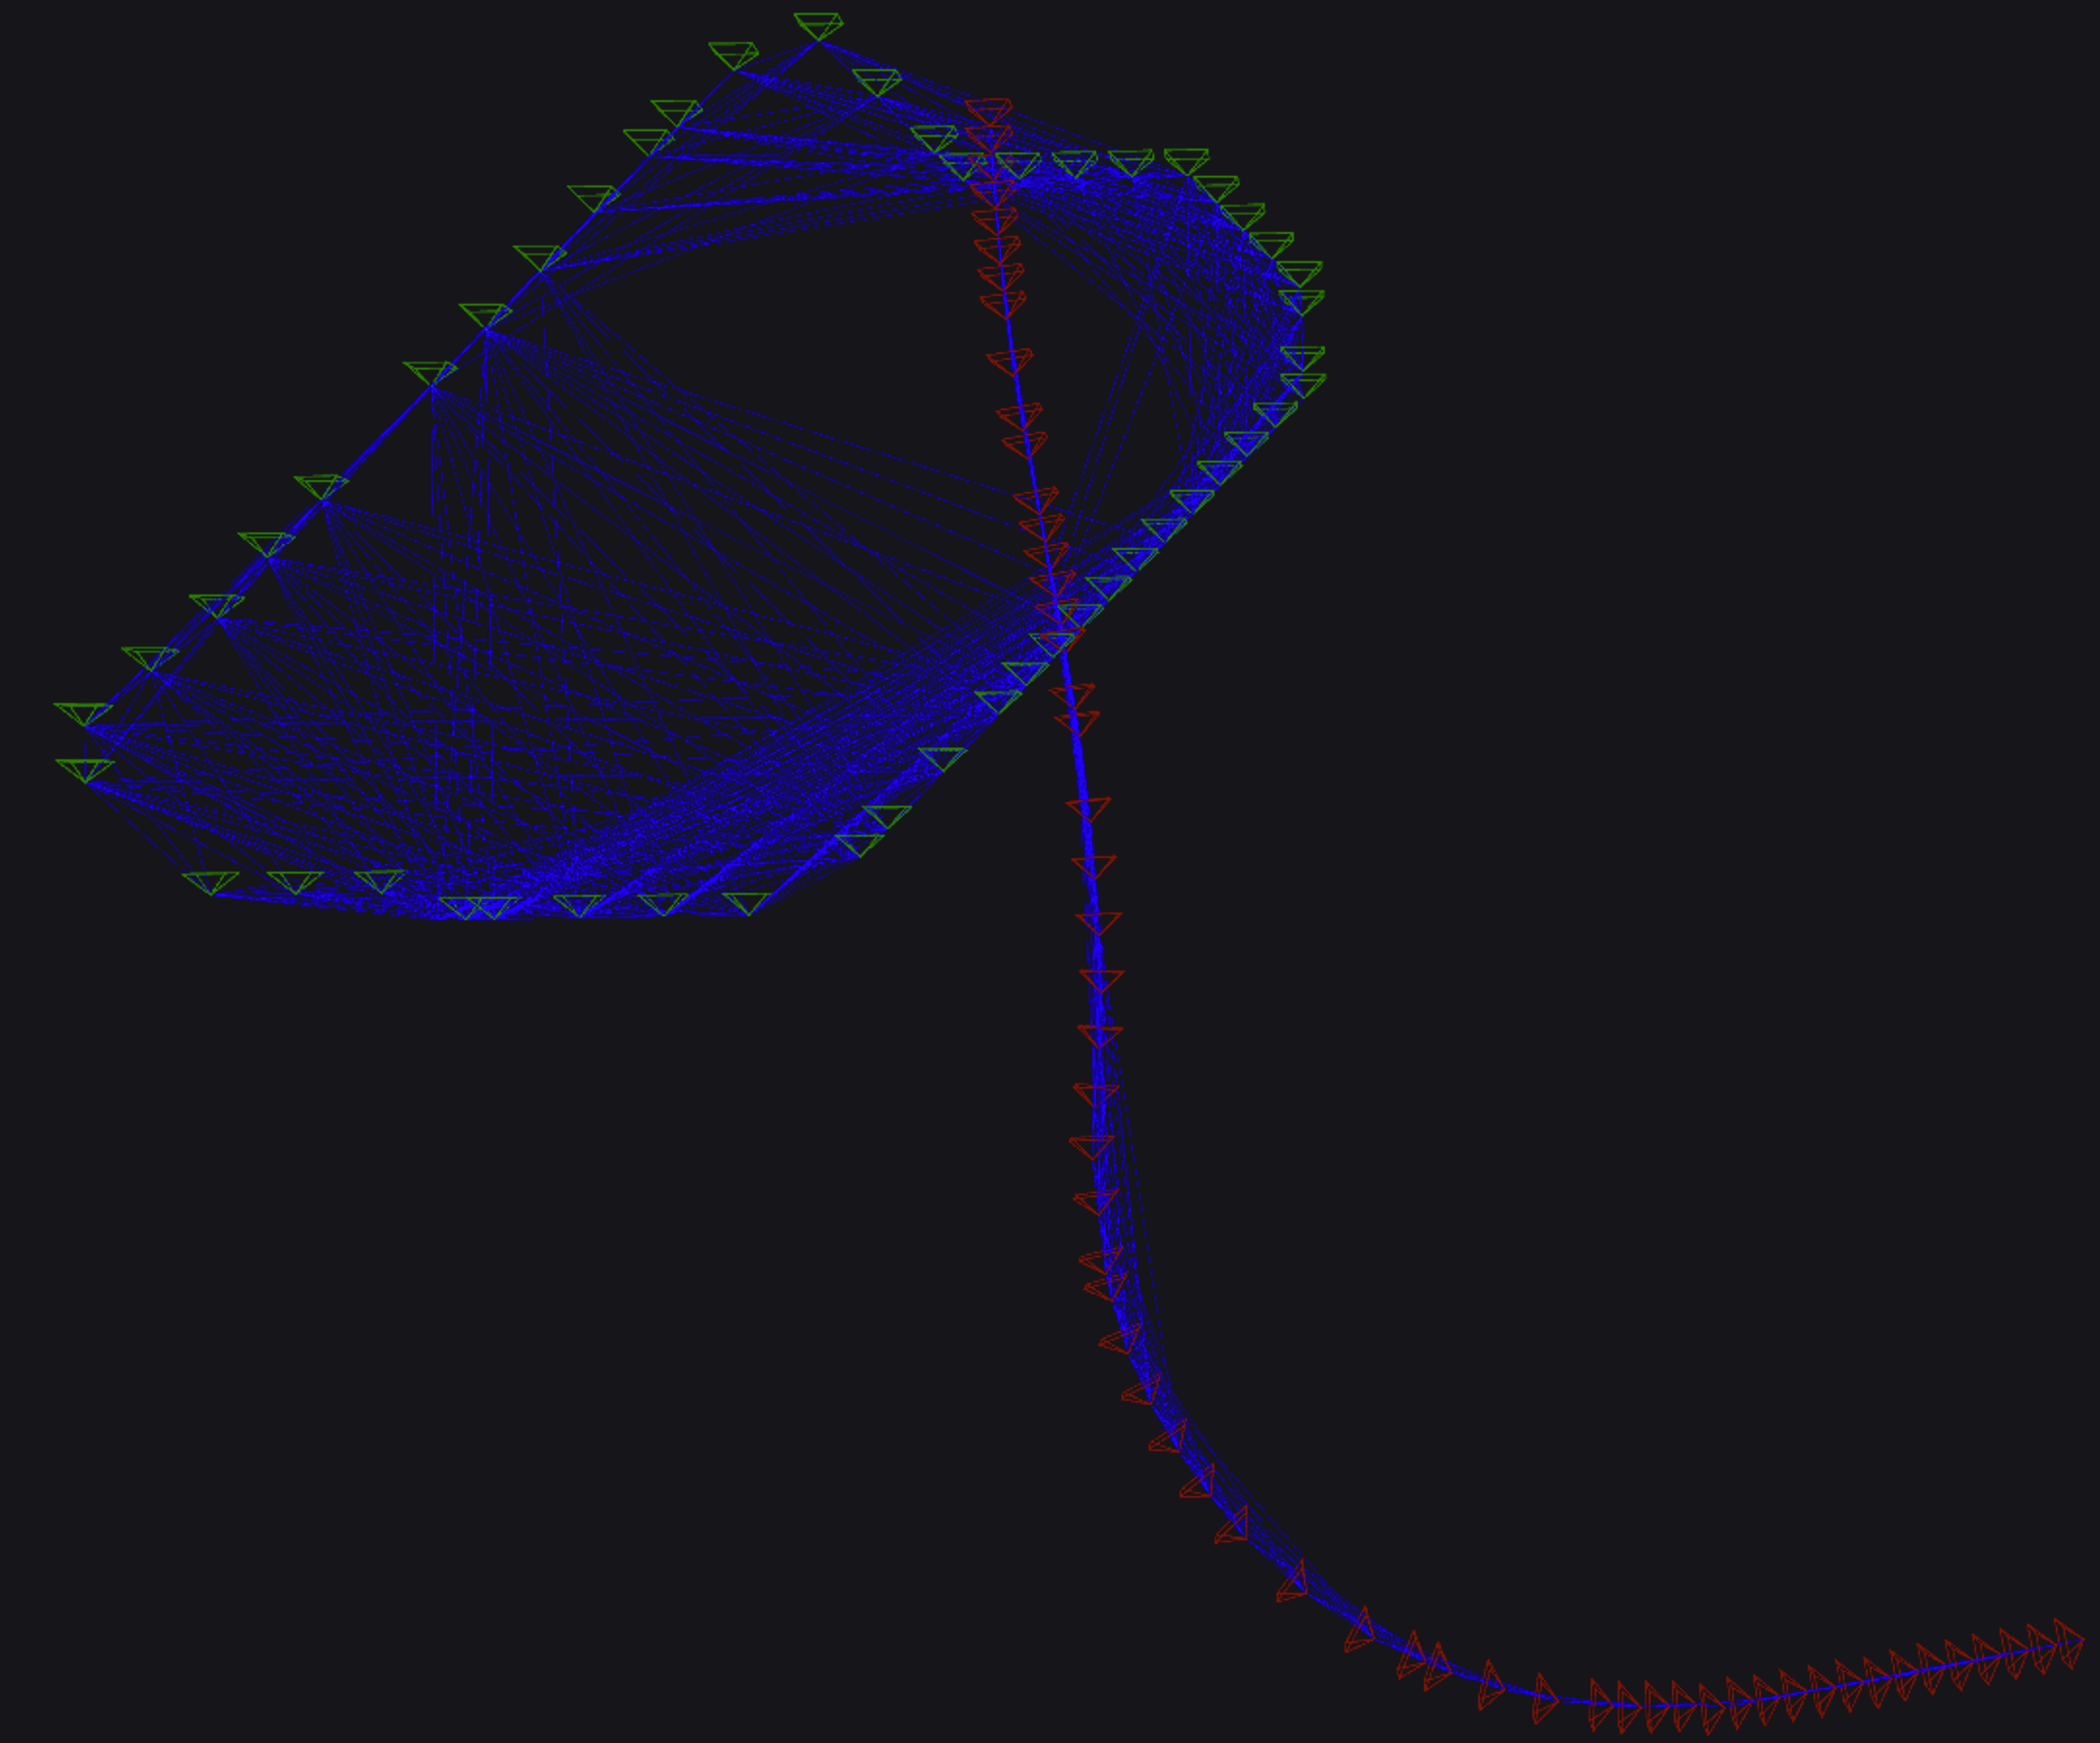
\includegraphics[width=\linewidth]{figures/after_merge.png}
        }
        \caption{Merged map}
    \end{subfigure}%

    \caption{Visual overview of the map merge process. We apply the translation $T_{loc \to ext}$ to the local map (a), and merge it with the external map (b), resulting in the merged map (c). The merged map contains information from both maps, creating our unified map. Note that the local map's scale also needs to be transformed, due to the arbitrary scale of monocular SLAM systems.}
    \label{fig:map-merge}

\end{figure}

The final version of the map merger works as follows:

\begin{enumerate}
    \item \textbf{Request external agent's full map.} \\
          Once a potential map merge with the external agent is identified by the \hyperref[sec:external-map-merge-finder]{external map merge finder}, we request its full map. Once the map is received, we deserialize it and temporarily place it into our \texttt{map database} data structure as a separate map.
    \item \textbf{Confirm that a map merge is possible using the full map data, and find the translation $T_{loc \rightarrow ext}$ that aligns the local map to the external map.} \\
          The visual word map merge finder identifies potential merges, however, we still need to confirm that a map merge is possible using the full map data from both agents. This is performed using a modified version of the ORB-SLAM3 loop closure detector.

          If we determine the merge to not be possible, we delete the external map from our map database and exit this process.
    \item \textbf{Apply translation $T_{loc \rightarrow ext}$ to our local map.} \\
          This shifts the local agent to be in the external agent's coordinate frame.
    \item \textbf{Move a subset of the external map's keyframes and map points into our local map} \\
          Given the external keyframe $k_0$ whose visual words triggered this map merge attempt, we extract a \textit{local window} $K_{wind}$ of keyframes connected to $k_0$ in the co-visibility graph and move them to our local map. Moving only a small number of keyframes at first allows the map point merge and pose graph optimization process to be completed faster, which is important as they block local mapping from being performed.
    \item \textbf{Merge local and external map points, connecting the maps}
    \item \textbf{Run pose graph optimization to optimize map point and keyframe positions.}
    \item \textbf{Repeat steps 5-7 with the entirety of the external map.}
    \item \textbf{Broadcast successful merge message.} \\
          If the full map merge is ultimately successful, we broadcast a \texttt{/successfully\_merged} message to tell our peers that we have successfully merged with the external agent. The external agent will then move to the \texttt{merged} state and both agents will begin sharing keyframes with each other, allowing the external agent to receive the local agent's full map.

\end{enumerate}

It is important to note that this system requires only one agent to identify and calculate the map merge, significantly reducing the computational overhead of map merging, especially in systems with many agents (further explained in the \nameref{sec:generalizing-to-n-geq-3-agent-systems} section).


\subsection{External KeyFrame Inserter}
\label{sec:external-key-frame-inserter}
Once the local and external agents have merged their maps and are in the same coordinate frame, they can begin sharing keyframes with each other.

Each agent maintains a set of unsent keyframes $K_{unsent}$ and map points $M_{unsent}$. Once $\#K_{unsent}$ exceeds a certain threshold, we serialize $K_{unsent}$ and $M_{unsent}$ and send them to the external agent. Finally, we set $K_{unsent} = \emptyset$ and $M_{unsent} = \emptyset$.

Upon receiving the serialized keyframes and map points, the external agent deserializes them and adds them to a queue to await insertion into their local copy of the shared map using the \texttt{external keyframe inserter}.

The external keyframe inserter is run whenever we have spare cycles on the CPU, to prevent impacting the local tracking and mapping performance. The insertion process involves the following operations:

(A concise visual overview of the process is presented in \autoref{fig:external-keyframe-inserter})

\begin{enumerate}
    \item \textbf{Pop $k_{ext}$ from the front of the external keyframe queue.}
    \item \textbf{Move $k_{ext}$ and its external observed map points $M_{ext}$ to the local map}. \\
          Since the local and external agents are merged, they are in the same coordinate frame. Therefore, we can move $k_{ext}$ and $M_{ext}$ to our local map without any transformations.\footnote[1]{I had previously used a \textit{keyframe anchor} method, where instead of $k_{ext}$ having an absolute pose we would send its pose relative to the previous $k_{ext}$. The thought process behind this was to prevent minor misalignments between the local and external maps from preventing external keyframes from properly integrating with the local map. However, experimental testing showed that this method instead caused the local and external maps to frequently diverge.}
    \item \textbf{Relink $k_{ext}$ with co-visible keyframes and observed map points in the local map}. \\
          $k_{ext}$ contains references to its co-visible keyframes and child map points that have already been sent or were generated by another agent. We search our local map for objects that match these references, reconnecting them.
    \item \textbf{Relink $M_{ext}$ with keyframes in the local map which observe it}. \\
          $M_{ext}$ contains references to keyframes that observe it which have already been sent or were generated by another agent. We search our local map for keyframes that match these references, reconnecting them.
    \item \textbf{Merge $M_{ext}$ with map points in the local map}. \\
          $M_{ext}$ will already be correctly linked to observing keyframes in the local map from step 4., however, due to communication latency some map points in $M_{ext}$ may be duplicates of existing map points in the local map. Therefore, we exploit spatial locality to merge duplicate map points that describe the same physical feature. A key observation from testing was that this step is essential to ensuring the local and external keyframes stay well connected, ensuring the local and external maps do not diverge.
    \item \textbf{Perform a local pose graph optimization around $k_{ext}$}. \\
          This optimizes our map using the new information we received from the external agent.
\end{enumerate}


\begin{figure}[h]
    \centering

    \begin{subfigure}[t]{0.3\textwidth}
        \centering
        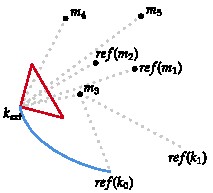
\includegraphics[height=1.9in]{figures/external_key_frame_insertion_1.pdf}
        \caption{External keyframe $k_{ext}$ with $M_{ext}=\{m_3, m_4, m_5\}$. Note the references to existing keyframes and map points.}
    \end{subfigure}%
    ~
    \begin{subfigure}[t]{0.3\textwidth}
        \centering
        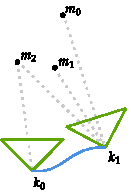
\includegraphics[height=1.9in]{figures/external_key_frame_insertion_2.pdf}
        \caption{Existing local map.}
    \end{subfigure}%
    \par\bigskip
    \begin{subfigure}[t]{0.333\textwidth}
        \centering
        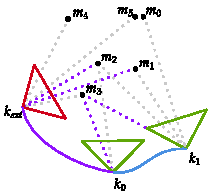
\includegraphics[height=1.9in]{figures/external_key_frame_insertion_3.pdf}
        \caption{\textbf{Step 2, 3\&4}: Move $k_{ext}$ and $M_{ext}$ to the local map and relink references. Relinked connections are drawn in purple.}
    \end{subfigure}%
    ~
    \begin{subfigure}[t]{0.333\textwidth}
        \centering
        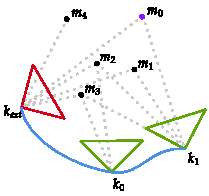
\includegraphics[height=1.9in]{figures/external_key_frame_insertion_4.pdf}
        \caption{\textbf{Step 5}: Merge duplicate map points. $m_5$ and $m_0$ have a similar feature descriptor and location, therefore they are merged.}
    \end{subfigure}%
    ~
    \begin{subfigure}[t]{0.333\textwidth}
        \centering
        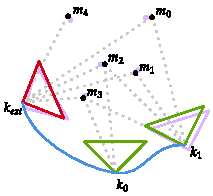
\includegraphics[height=1.9in]{figures/external_key_frame_insertion_5.pdf}
        \caption{\textbf{Step 6}: Local pose graph optimization around $k_{ext}$ to refine the map using the new information. Original keyframe and map point locations are shown in purple.}
    \end{subfigure}%

    \caption{Visual overview of inserting external keyframes and map points into the local map. External keyframe (a) and initial local map (b) are combined to create our final local map (e).}
    \label{fig:external-keyframe-inserter}

\end{figure}


\subsection{Local KeyFrame Inserter}
\label{sec:local-key-frame-inserter}
As mentioned in the \nameref{sec:external-key-frame-inserter} section, it is essential that the local and external maps stay well connected, sharing the majority of their map points. In other words, we must ensure that the external map data is integrated throughout the entire SLAM pipeline.

The \texttt{Tracking} and \texttt{Mapping} modules, which are responsible for localizing the robot and generating new keyframes, only interact with the \texttt{Map Database}, as seen in the previously shown architectural diagram in \autoref{fig:agent-diagram}. Our external keyframe inserter does all the work of properly reconnecting external map points and merging duplicate map points, leaving the \texttt{Map Database} data structure looking as if all the map points and keyframes were generated locally. This abstracts the \texttt{Tracking} and \texttt{Mapping} modules away from the distributed aspects of the system, ensuring that they fully utilize the external map points when localizing the agent and generating new keyframes (\autoref{fig:well-connected-graph}).


\begin{figure}[h]
    \centering
    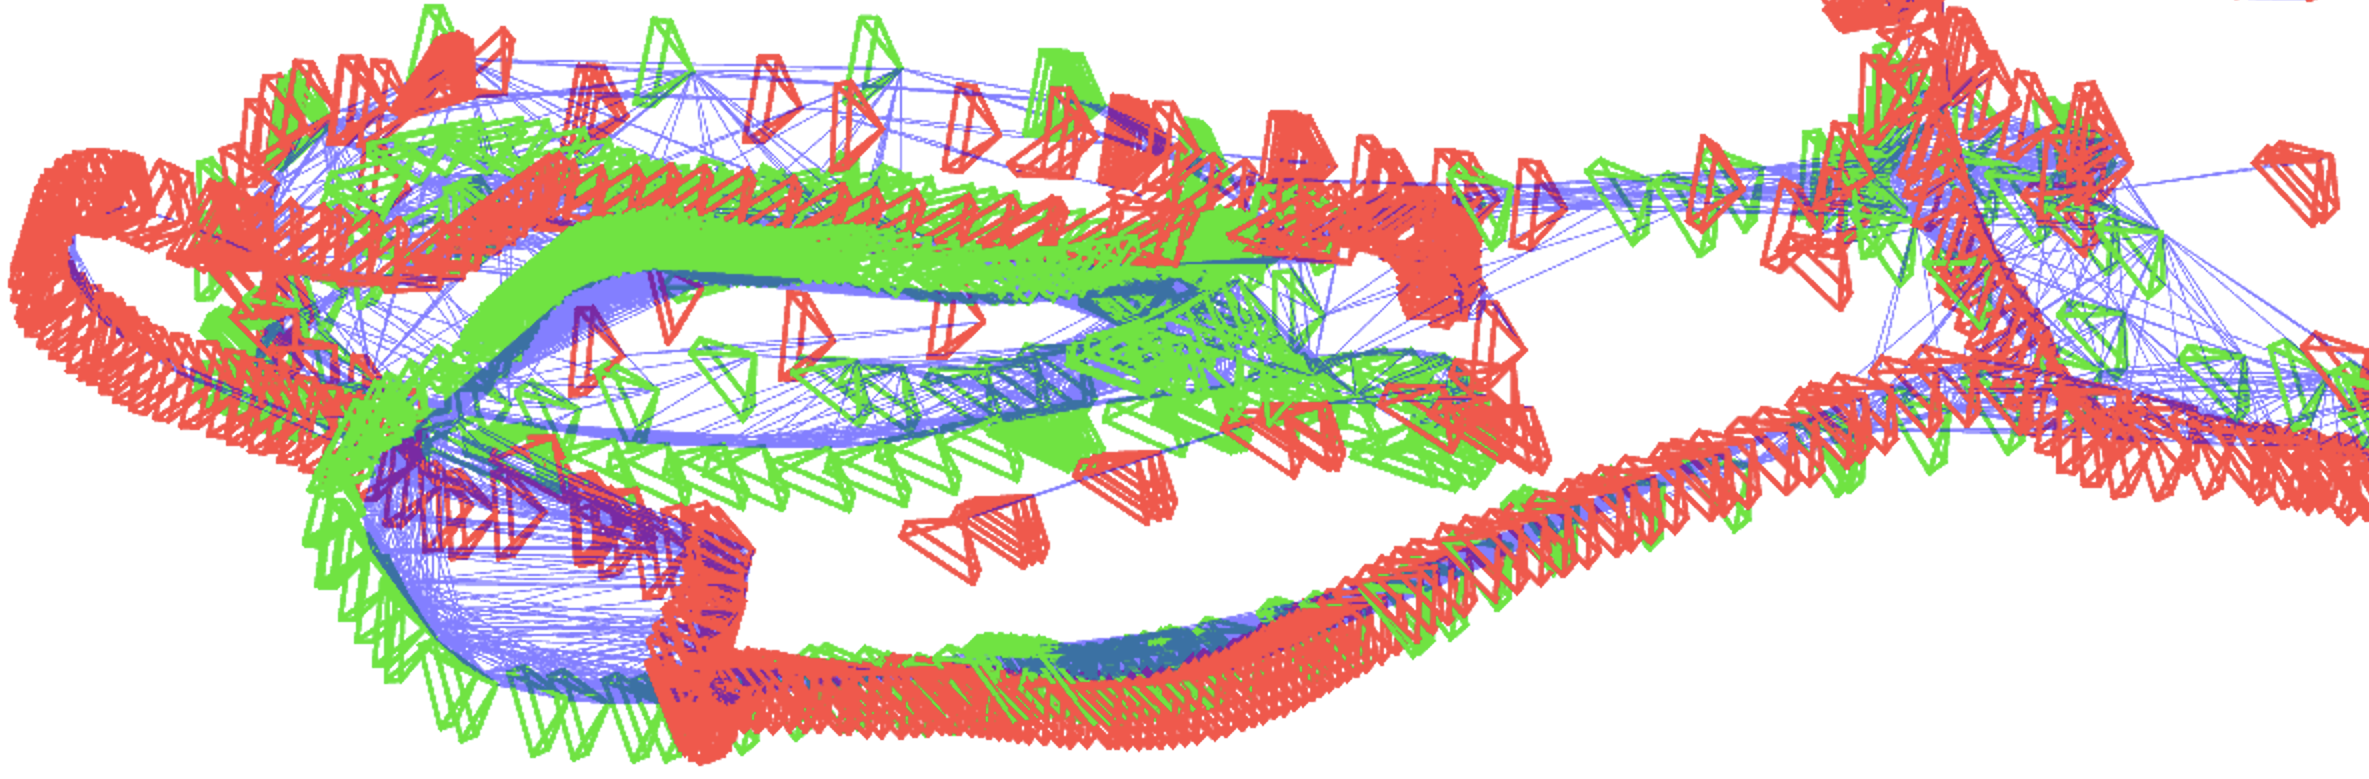
\includegraphics[width=0.8\linewidth]{figures/map_integration.png}

    \caption{Section of the keyframes generated when running the EuRoC Machine Hall dataset. The local (green) and external (red) keyframes are well connected by co-visibility links (blue), demonstrating that they are tracking the same map points.}
    \label{fig:well-connected-graph}
\end{figure}

\subsection{Generalizing to $N \geq 3$ Agent Systems}
\label{sec:generalizing-to-n-geq-3-agent-systems}
Now that we have explained how a pair of agents interact, we can explore how this can be generalized to a system with an arbitrary number of agents.

We assume a system with $N$ agents $A=\{agent_1, agent_2, ..., agent_N\}$, where $agent_i$ is the agent with ID = i. Within this system we maintain a state $S_i=state_{n-m}$ for every agent pair $(agent_n, agent_m)$, giving us a total of $N(N-1)/2$ states. We also have a set $G$ which contains all the groups of merged agents. The \textit{group leader} is defined as the agent in a group with the lowest agentId.

In the case where agents can lose communication with one another, we also assume that if any given $agent_n$ is able to communicate with an $agent_m$, $agent_n$ can also communicate with all of $agent_m$'s connected peers. This is held if the agents are using a mesh network to communicate, for example.

Initially, every agent pair is unmerged so every state in $S$ is set as \textit{unmerged} and $G=\{\{agent_1\}, \{agent_2\}, ..., \{agent_N\}\}$

A key insight of my distributed SLAM system is to delegate all merge operations to group leaders. This is significant, as the computational load and bandwidth requirements of these merge operations scale proportional to the square of the number of agents involved, and in most use cases the number of group leaders quickly drops to be much lower than the total number of agents. Additionally, having all merge operations performed by the group leader prevents potential race conditions introduced by communication latency within a group, for example, two agents within a group merging with different agents at the same time.

As discussed in the \hyperref[sec:external-map-merge-finder]{External Map Merge Finder} and \hyperref[sec:external-map-merger]{External Map Merger} sections, the two operations needed to merge are (1) exchanging visual words to identify visual overlap and therefore merge opportunities and (2) sending over the map and attempting a full map merge. Our group leaders must therefore perform these tasks on behalf of their groups.

The ``visual word merge finder'' operation can be delegated to group leaders by having them send the visual words of all keyframes generated by agents within their group to all other group leaders. This introduces no additional intra-group communication, as all agents within a group already send each other all new keyframes.

Moving on to the ``full map merge'' operation, once a pair of group leaders $(agent_n, agent_m)$ (with $n<m$) have found a potential merge using visual words, the agent with the smaller ID ($agent_n$) sends its full map to the agent with the larger ID ($agent_m$), who attempts a full map merge. If the merge is successful, $agent_m$ will now be in $agent_n$'s coordinate frame. $agent_m$ will then send the transform from $agent_m$ to $agent_n$'s coordinate frame $T_{m \to n}$ to all the agents in its group, allowing them to also change to $agent_n$'s coordinate frame. After this has been completed, $agent_m$'s group merges into $agent_n$'s group by updating $S$ according to \autoref{eq:state-update-equation}, and agents begin exchanging keyframes to update the unified map.

\begin{equation}
    \begin{gathered} \label{eq:state-update-equation}
        \forall i \in g_n. \ \forall j \in g_m. \ state_{i-j} \in S \text{ and } state_{i-j} = ``merged" \\ \text{where $g_n, g_m \in G$ are the groups that $agent_n$ and $agent_m$ respectively lead.}
    \end{gathered}
\end{equation}

This approach requires all agents to know the current groups and group leaders within the decentralized system, which is achieved by broadcasting all successful merge messages on the \texttt{/successfully\_merged} ROS topic for everyone to see.

This whole process is perhaps best represented in visual form by the simple 3-agent merge example given in \autoref{fig:3-agent-merge} which shows the messages sent between agents.

\begin{figure}[h]
    \centering
    \captionsetup{format=plain}
    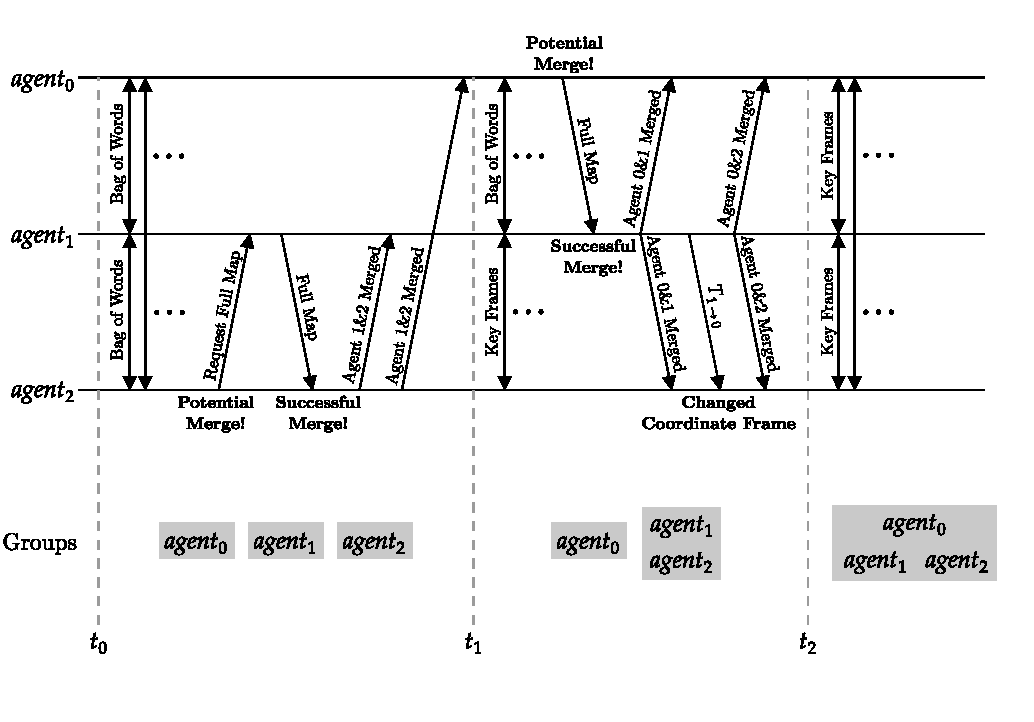
\includegraphics[]{figures/3_agent_merge.pdf}

    \caption{This is a simple 3 agent merge example where $agent_1$ and $agent_2$ merge first, and then $agent_0$ and $agent_1$. Agents in the same group are shown in the same rectangle, with the group leaders bolded. \captionbreak Initially at $t_0$, all agents are unmerged. Therefore, they are all group leaders and share the ``bag of words'' representations of new keyframes with each other. $agent_2$ then finds a potential merge with $agent_1$. The lower agent ($agent_1$) sends $agent_2$ its full map, who successfully merges with it, transforming it into $agent_1$'s coordinate frame. \captionbreak At $t_1$, $agent_1$ and $agent_2$ are merged and therefore begin exchanging keyframes. $agent_0$ and $agent_1$ are the two remaining group leaders, so they continue to exchange their ``bag of words''. $agent_0$ detects a potential merge with $agent_1$, and since $0<1$ it sends its full map to $agent_1$. $agent_1$ successfully merges with $agent_0$'s full map, so it sends the transform $T_{1 \to 0}$ ($agent_1$ to $agent_0$'s coordinate frame) to all members of its group. This allows $agent_2$ to change from $agent_1$ to $agent_0$'s coordinate frame. \captionbreak At $t_2$, all three agents are merged and in $agent_0$'s coordinate frame. Therefore they all exchange keyframes with one another. \captionbreak This example is slightly simplified as all potential merges result in successful full merges. In reality, multiple potential merges may be identified before two agents successfully merge.}
    \label{fig:3-agent-merge}
\end{figure}

\subsection{Map Alignment Refiner}
\label{sec:map-alignment-refiner}
As our shared map grows, our local map may ``fall out of alignment''. In other words, the map is slightly translated, rotated, or scaled with respect to the lead agent's map. This is largely a side effect of our aggressive early merge strategy which may merge two agents' maps before there is significant overlap, causing the estimated map alignment to have some error. These small alignment errors are completely acceptable when maps are small, but may cause the maps to diverge as they grow.

To remedy this problem, we continuously refine our map alignment using the \nameref{sec:ransac} and \hyperref[sec:kabsch-umeyama-algorithm]{Kabsch-Umeyama point set alignment} algorithms. Map alignment is performed as follows:

\begin{enumerate}
    \item \textbf{Request map point locations from the lead agent}. \\
          This is defined as the set TaggedMP$_{ext}$ where TaggedMP${_{ext}}_i = (\text{uuid}, (x, y, z))$
    \item \textbf{Extract local map point locations}. \\
          This is defined as the set TaggedMP$_{local}$ where TaggedMP${_{local}}_i = (\text{uuid}, (x, y, z))$
    \item \textbf{Use RANSAC with the Kabsch-Umeyama algorithm to find the transform $T_{local \to ext}$ which best aligns TaggedMP$_{local}$ to TaggedMP$_{ext}$.} \\
          The \hyperref[sec:kabsch-umeyama-algorithm]{Kabsch-Umeyama} algorithm finds the SIM(3) transformation $T_{local \to ext}$ from TaggedMP$_{ext}$ to TaggedMP$_{local}$, minimizing the root mean squared error. However, our input data may contain a large number of outliers so we use \nameref{sec:ransac} to find a good fit while ignoring outliers.
    \item \textbf{Apply transformation $T_{local \to ext}$ to our local map to realign it with the group leader.}
\end{enumerate}

We use an \textit{additive increase multiplicative decrease} methodology to control how often map alignment is performed. Given $t_i$ is the time between the $i$-th and $(i+1)$-th map alignments, we set $t_{i+1} = t_i + 1$ if the maps were well aligned, and $t_{i+1} = t_i / 2$ if the maps were not well aligned. This prevents agents from continuously performing map alignments when their maps are already well aligned.

\subsection{Losing Localization / Connection}
\label{sec:losing-localization-or-connection}
An agent can lose localization within the shared map (for example, if its camera is blocked for a short period of time). When this happens, the agent signals to its peers that it has lost localization and they stop sharing new keyframes. Since the agent has lost localization in the shared map, it begins building a private map of the new area it is observing. If it revisits an area of the shared map, it will merge its private map with the shared map and signal to its peers that it has regained localization. Keyframe sharing will then resume, with the agents' unsent keyframes being sent to one another. This allows the new area explored while localization was lost to expand the shared map.

Losing connection is very similar, however, a new private map does not need to be built. Instead, the agents simply stop sharing keyframes until the connection is regained, at which point the agents will update each other with the stored-up unsent keyframes.

\subsection{Visualization Publisher}
\label{sec:visualization-publisher}
All 3D visualizations are created by publishing ROS markers, a standardized ROS message type that represents some object in 3D space such as lines, points, or meshes. These ROS markers can then be displayed by a variety of third-party visualization tools such as RViz \autocite{10.1007/s11235-015-0034-5} and Foxglove Studio \autocite{foxgloveStudio}.

Using ROS markers allows me to leverage these mature visualization tools instead of creating one from scratch, and also allows visualizations to be easily saved and replayed for later analysis. Demonstrations of these 3D visualizations can be found in the supplementary video\footnote[1]{Supplementary video URL: \url{https://cam-diss.s3.amazonaws.com/video.mp4}}

\section{Motion Controller}
\label{sec:motion-controller}
While not a part of the core SLAM system, the motion controller node closes the control loop and provides real-world demonstrations of my system. From a high level, the motion controller node consumes the local and external agents' poses and outputs a command velocity to the robot's movement system – all via ROS topics. For this project, I have implemented two different motion control systems which can be switched between seamlessly.

\subsection{Follow The Leader}
\label{sec:follow-the-leader}
The \textit{follow the leader} motion controller consists of two agents: one leader and one follower. The follower is given a position and rotation offset to the leader which it attempts to maintain as the leader is moved around.

% For example, you could set the follower to be 1 meter behind the leader with a 180\textdegree{} rotational offset. This would mean the leader and follower never have visual overlap at any given moment, demonstrating that my SLAM system is truly building a shared map.

% Spinning the agents around in a circle demonstrates that the two agents' maps are properly merged and that the agents are using map points generated by an external agent to localize themselves, giving accurate relative positioning even when there is no visual overlap at any given moment.

% \comment{TODO: add figure of the map built}

\subsection{Multi-Agent Collision Avoidance}
\label{sec:multi-agent-collision-avoidance-implementation}
The \textit{multi-agent collision avoidance} example is more complex, employing a non-linear model predictive controller (NMPC) to avoid collisions with both static and dynamic obstacles. My NMPC system is improved version of \autocite{DBLP:journals/corr/KamelASN17} and is defined as follows:

\subsubsection{Non-Linear Model Predictive Controller Formulation}
\label{sec:nmpc-controller-formulation}
We assume an agent with current pose $\bm{p} \in \mathbb{R}^2$ and radius $r$. Firstly, we define our agent's control input $\bm{v_{cmd}}$ as a function describing its velocity over time. We can then define our agent's state as a function of time $\bm{x}(t)$ as the control input $\bm{v_{cmd}}$ applied to its current pose $\bm{p}$:

\begin{equation}
    \bm{x}(t) = \bm{p} + \int_{0}^{t} \bm{v_{cmd}}\ dt
\end{equation}

Solving the following minimization problem will yeild an optimal $\bm{v_{cmd}}$:
\begin{equation}
    \begin{aligned} \label{eq:nmpc-minimization-problem}
         & \min_{\bm{v_{cmd}}} \int_{t=0}^{T} J_x(\bm{x}(t), \bm{x_{ref}}(t)) + J_s(\bm{x}(t)) + J_d(\bm{x}(t))\ dt \\
         & \text{subject to } \bm{v_{min}} \leq \bm{v_{cmd}} \leq \bm{v_{max}}
    \end{aligned}
\end{equation}
where $T$ is our horizon length, $\bm{x_{ref}}$ is our target trajectory, and $J_x$, $J_s$, $J_d$ are the cost functions for this system.

Cost function $J_x$ rewards following the target trajectory $\bm{x_{ref}}$ and is shown below:
\begin{equation}
    J_x(\bm{x}, \bm{x_{ref}}) = \|\bm{x} - \bm{x_{ref}}\|^2
\end{equation}

$J_s$ and $J_d$ penalize collisions with static objects and dynamic objects respectively. They are defined as:
\begin{flalign}
    J_s(\bm{x}) & = \sum_{i=1}^{N_{static}} \frac{s_s*Q_s}{1 + \exp(d_i^{static} / s_s)}   \\
    J_d(\bm{x}) & = \sum_{i=1}^{N_{dynamic}} \frac{s_d*Q_d}{1 + \exp(d_i^{dynamic} / s_d)}
\end{flalign}
where $d_i^{static}$ is the distance between the agent and the $i-th$ static obstacle, and $d_i^{dynamic}$ is the distance between the agent and the $i-th$ dynamic obstacle. $Q_s>0$ and $Q_d>0$ are weights that define how adverse our agents are to collision with static and dynamic obstacles respectively. A visualization of how these parameters affect the cost function is presented in \autoref{fig:nmpc_cost_function-a}.

Additionally, we define $s_s$ and $s_d$ as scale normalizing parameters that ensure the minima of $J_x + J_s$ and $J_x + J_d$ are invariant to $Q_s$ and $Q_d$. To calculate $s_s$, we first find the positive minima $x_{min}$ of $J_x + J_s$ in the worst case where $d_i^{static} = J_x$ (ie. the static obstacle and $x_{ref}$ are at the same place), with $s=1$. This gives us $x_{min}$ as defined in \autoref{eq:x-min}. Our scaling factor can then be defined as $s_s = \frac{r}{x_{min}}$, which sets the positive minima of $J_x + J_s$ to be $r$ in the above situation. The calculation of $s_d$ is symmetric, simply using $Q_d$ instead of $Q_s$.

\begin{equation} \label{eq:x-min}
    x_{min} = \ln \left( \frac{\sqrt{Q_s^2-4Q_s}+Q_s}{2}-1 \right)
\end{equation}

The key benefit of these cost functions is that the optimal distance to obstacles is kept at the collision point, and is invariant to parameters $Q_s$ and $Q_d$. This is in contrast to \autocite{DBLP:journals/corr/KamelASN17} which requires the parameters $\kappa$ and $Q$ to be re-tuned after changing agent radius $r$. This is because their cost functions do not have their minima at the collision point, but instead at some point before the collision that varies with $\kappa$, $Q$, and $r$, making them very difficult to tune. This is visualized in \autoref{fig:nmpc_cost_function}

% TODO could be explained better idk

\begin{figure}[h]
    \centering

    \begin{subfigure}[t]{0.33\textwidth}
        \centering
        \caption{My Cost Function}
        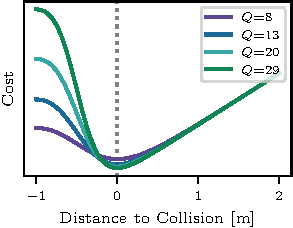
\includegraphics[height=1.7in]{figures/nmpc_cost_function_0.pdf}
        \label{fig:nmpc_cost_function-a}
    \end{subfigure}%
    ~
    \begin{subfigure}[t]{0.33\textwidth}
        \centering
        \caption{Kamel et al.'s Cost Function}
        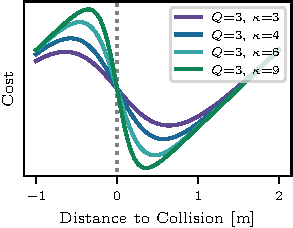
\includegraphics[height=1.7in]{figures/nmpc_cost_function_1.pdf}
    \end{subfigure}%
    ~
    \begin{subfigure}[t]{0.33\textwidth}
        \centering
        \caption{Kamel et al.'s Cost Function}
        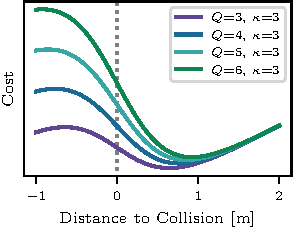
\includegraphics[height=1.7in]{figures/nmpc_cost_function_2.pdf}
    \end{subfigure}%

    \caption{Comparison of my cost function (a) and Kamel et al.'s cost function (b), (c) when the obstacle and goal pose are at the same location. This demonstrates that my cost function's minima is always at the collision point and does not vary as the parameters are changed, as opposed to Kamel et al.'s function.}
    \label{fig:nmpc_cost_function}
\end{figure}

\subsubsection{Implementation Details}
\label{sec:nmpc-implementation-details}
Solving the integral in \autoref{eq:nmpc-minimization-problem} is computationally inefficient, therefore we split our calculations into discrete time steps. Specifically, the time horizon is set as $T=500ms$ with $100ms$ timesteps.

The \textit{Sequential Least Squares Programming} minimization method is used due to its robustness and ability to constrain the optimization space, which we use to keep $\bm{v_{min}} \leq \bm{v_{cmd}} \leq \bm{v_{max}}$. We set parameters $Q_s = 8$ and $Q_d = 12$ to make the agent more adverse to approaching dynamic obstacles than static ones, as there is more uncertainty in the dynamic obstacle's location. To calculate the future locations of dynamic obstacles $\bm{x_i^{dynamic}}(t)$ we employ a simple constant velocity model.

% Our SLAM system does not use a depth camera or LiDAR, and therefore only produces a sparse map. Consequently, we need to define the location of static obstacles manually. Both static obstacles and the goal pose are set using interactive ROS markers, allowing them to be changed ``on the fly" using software such as RViz.

\section{Central Management Interface}
\label{sec:central-management-interface}
While my multi-agent system is fully decentralized, a significant amount of work was put into developing the supporting infrastructure needed to control, test, and evaluate this system. The primary method of managing the distributed system is through the cross-platform \textit{Central Management Interface}, which can be used to: \noparskip
\smallbreak
{
    \begin{enumerate}
        \item \textbf{Manually control the agent's poses.} \\
              Users can click and drag on an image in area 1 to rotate the agent's camera and use the keyboard to move the agent around.
        \item \textbf{Record camera data from the simulation software.}
        \item \textbf{Play datasets back for testing and benchmarking purposes.}
        \item \textbf{Record trajectories generated by the SLAM system as well as ground truth data for later evaluation.} \\
              The recorded trajectory data can later be ingested by my custom evaluation library Multi-Agent Evo for analysis.
    \end{enumerate}
}

\begin{figure}[h]
    \centering
    \begin{subfigure}[t]{0.425\textwidth}
        \centering
        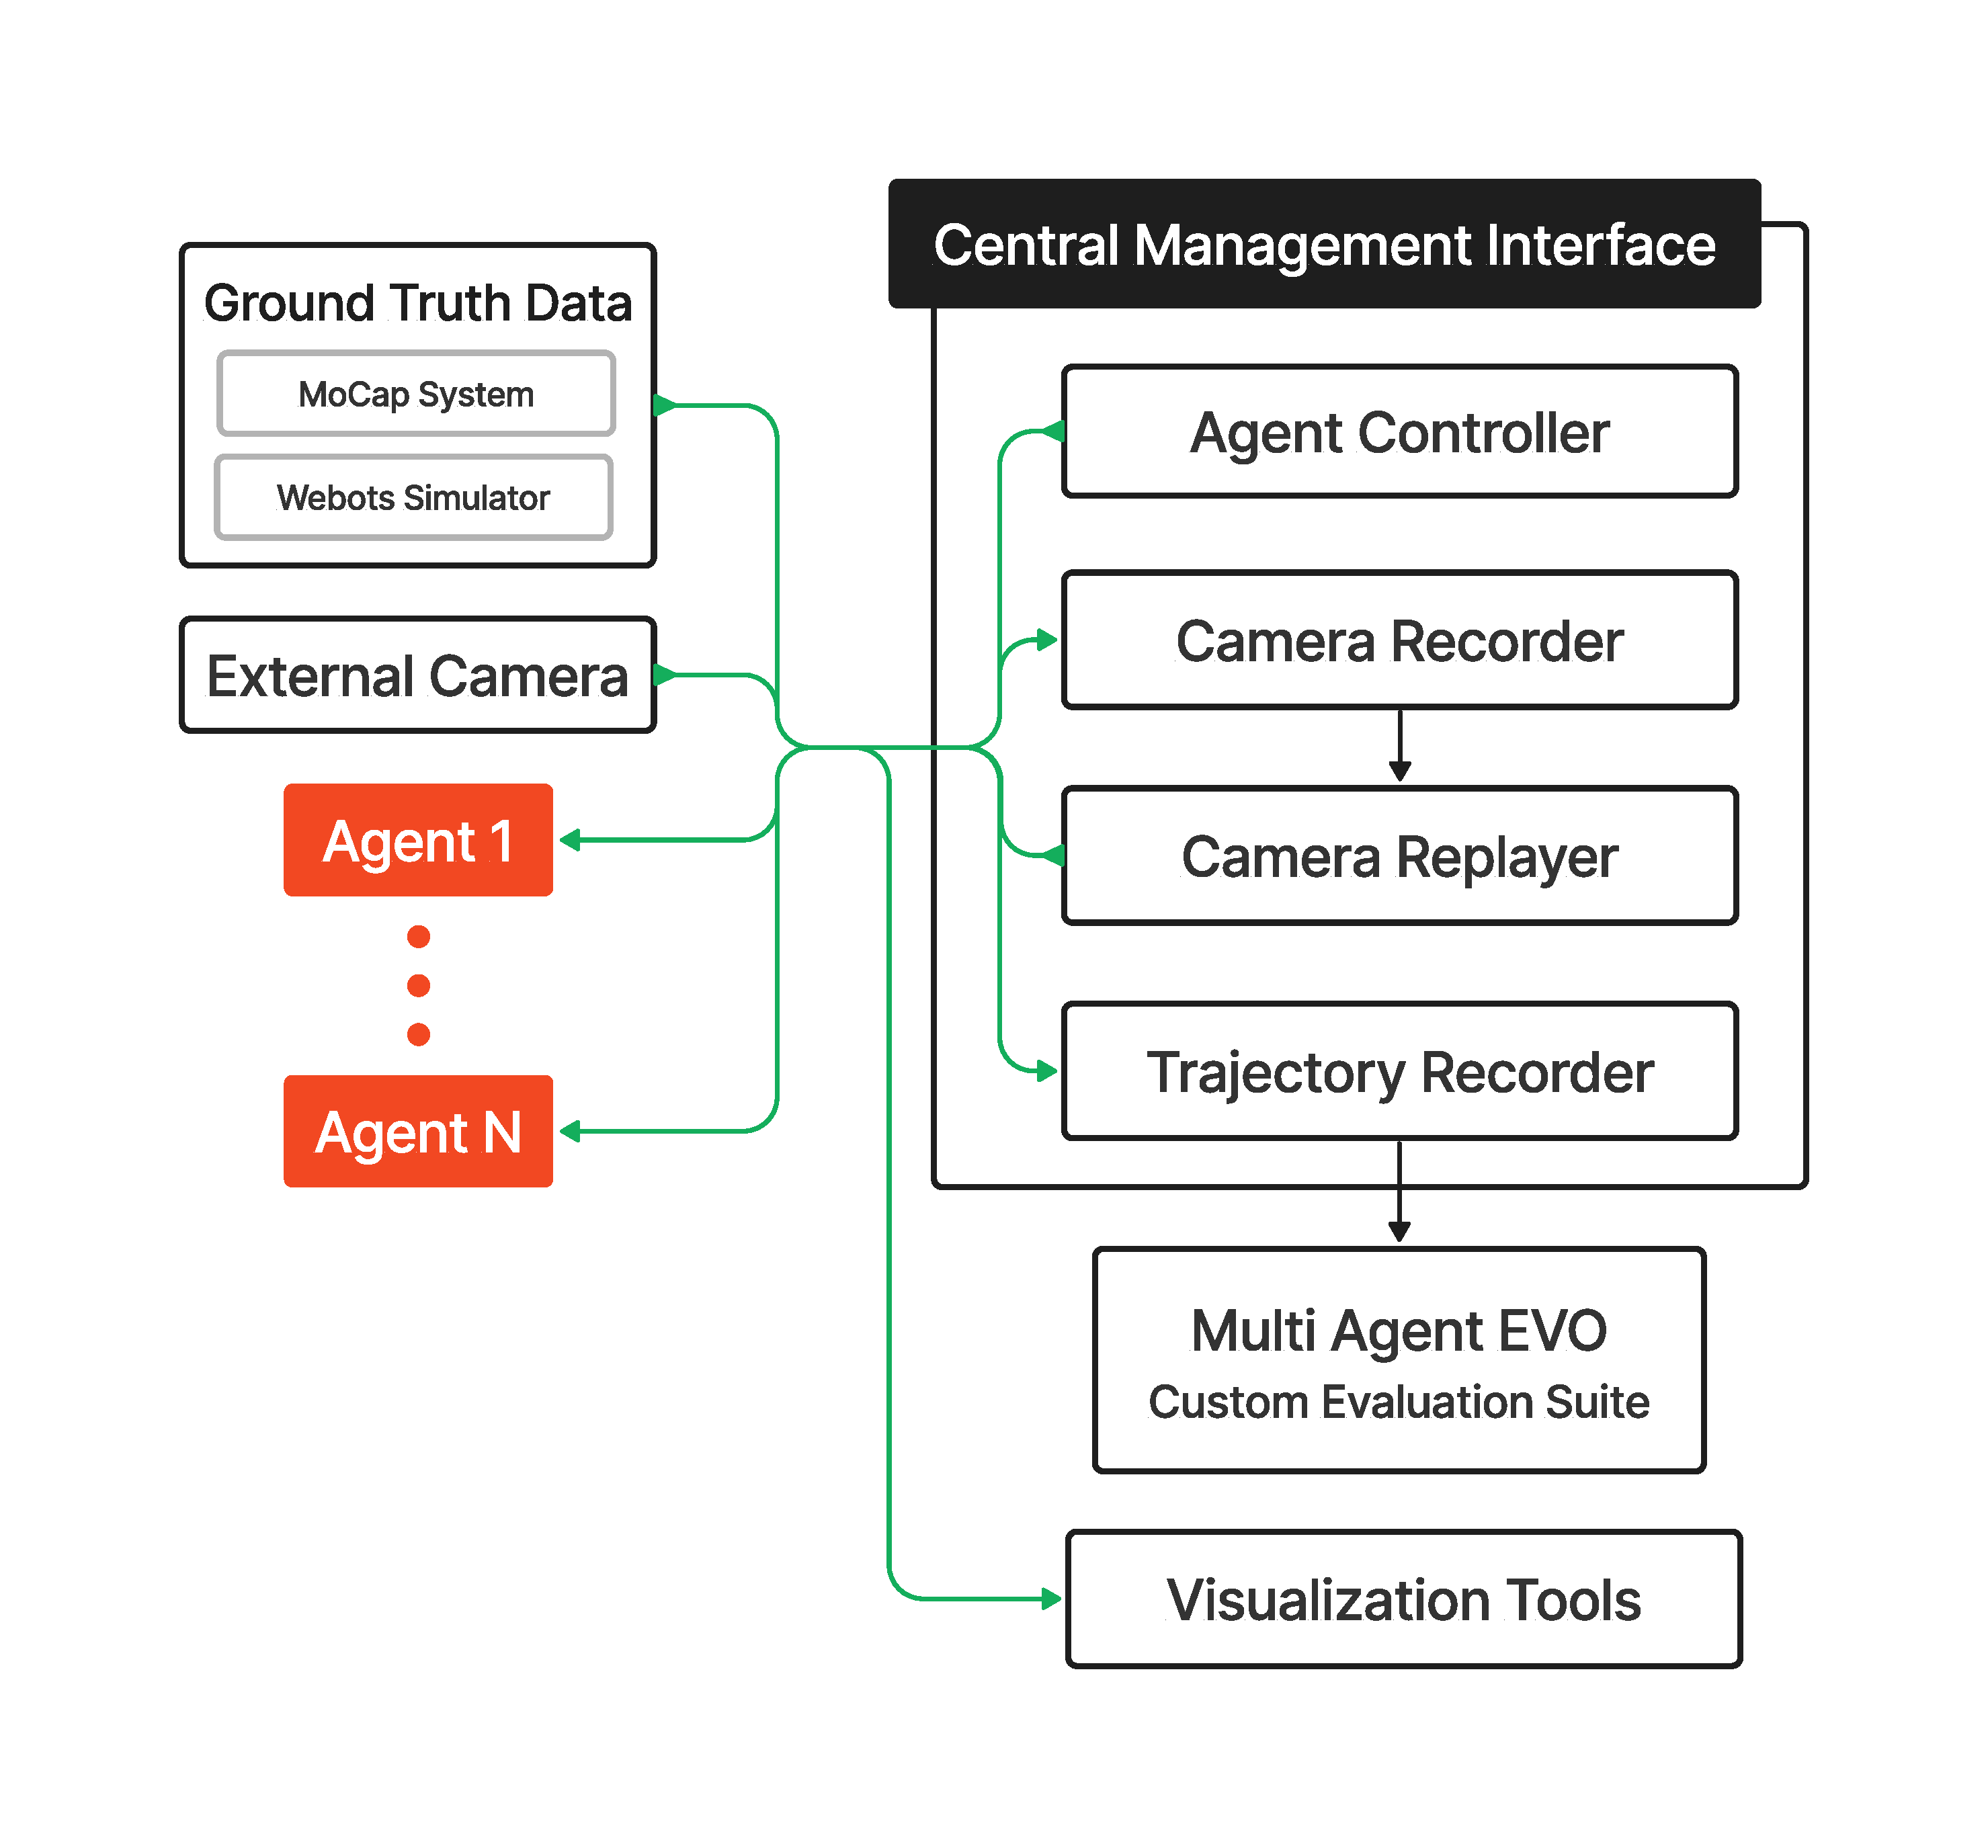
\includegraphics[trim=5cm 0cm 5cm 5cm, width=\linewidth]{figures/central_management_interface_diagram.pdf}
        \caption{Central Management Interface architectural diagram}
    \end{subfigure}\hfill%
    ~
    \begin{subfigure}[t]{0.5\textwidth}
        \centering
        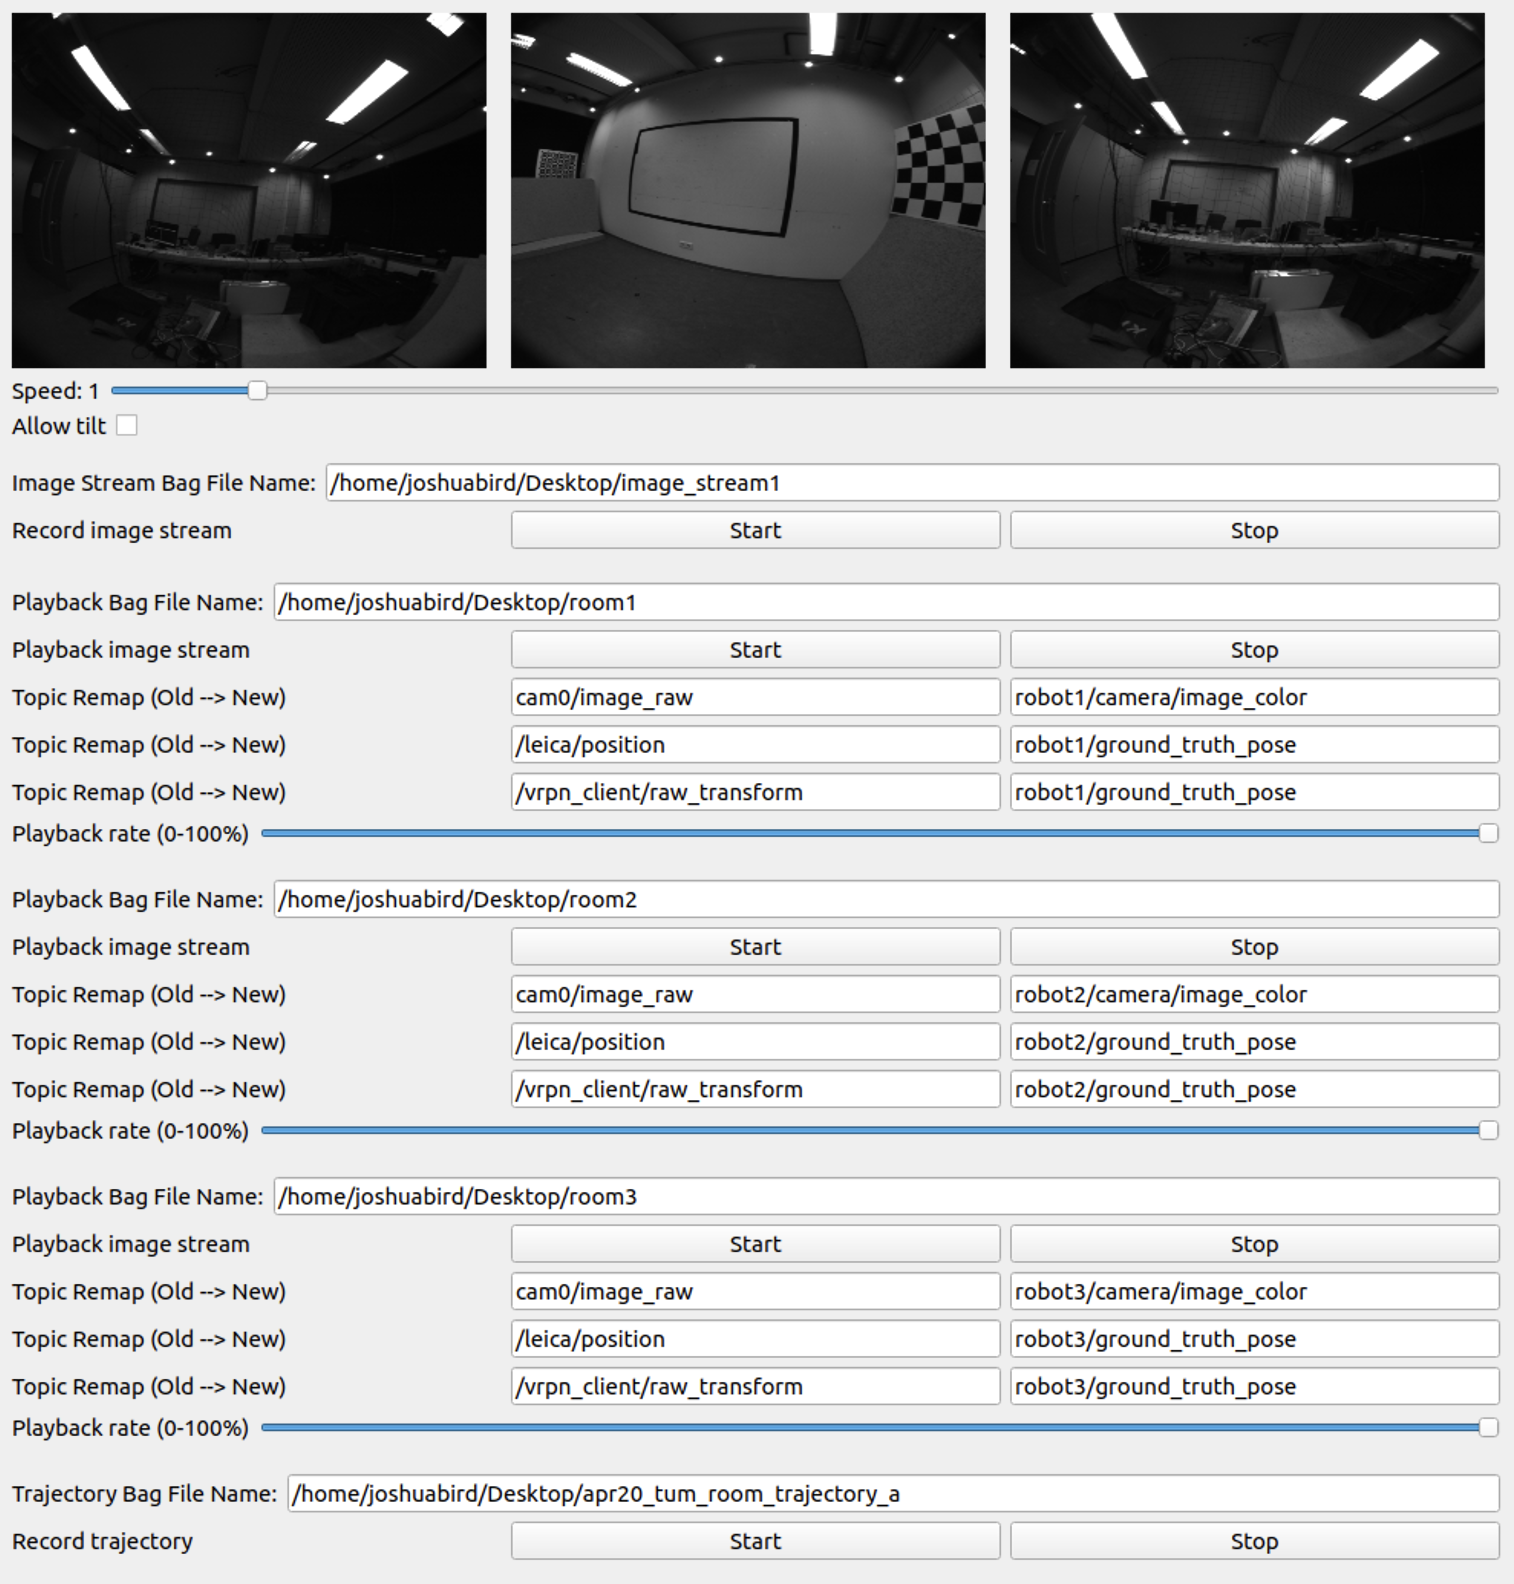
\includegraphics[trim=5cm 3cm 5cm 5cm, width=\linewidth]{figures/central_management_interface.pdf}
        \caption{Central Management Interface}
    \end{subfigure}%

    \caption{The central management interface, used for controlling agents, recording datasets, playing back datasets, and recording trajectories for later analysis.}
    \label{fig:central-management-interface}
\end{figure}

As a result of abstracting implementation details behind ROS topics, this central management interface is able to work seamlessly with both agents running in a simulator and agents running on real-world robots.

\section{Custom Evaluation Suite – Multi-Agent EVO}
\label{sec:multi-agent-evo}
While there are several mature single-agent SLAM evaluation tools, I found there to be a complete lack of evaluation tools for multi-agent SLAM systems – to the best of my knowledge no papers have published their evaluation code. Therefore, I have created an open-source multi-agent SLAM evaluation tool: \textit{Multi-Agent EVO}, based on the popular single-agent SLAM evaluation tool \textit{EVO} \autocite{grupp2017evo}.

In addition to the data structures and data ingestion modifications needed for EVO to process multi-agent SLAM data, evaluating data from a multi-agent system introduces some additional complexities.

Initially, all agents are in separate reference frames until they merge their maps and begin sharing the same coordinate frame. We may also have cases where two independent groups of agents meet and merge maps, which requires multiple agents to simultaneously change coordinate frames.

Therefore, I have created a new data format to capture these changes in coordinate frames over time within our trajectory data, which Multi-Agent EVO is able to ingest. This allows us to properly compare the multi-agent SLAM trajectories to the ground truth data, giving us insights into how long it takes for agents to successfully merge maps, the accuracy of relative pose estimation, and much more.

Once agents $m$ and $n$ merge, they publish the translation $T_{m \to n}$ to the \texttt{sim3\_transform} ROS topic. When we go to evaluate the trajectory error, Multi-Agent EVO ingests the \texttt{sim3\_transform} data to build a directed acyclic graph (DAG) of all merged agents, as shown in \autoref{fig:evo-coord-frames}. This DAG can then be used to find if agents are merged with each other, and the transform between their coordinate frames. We then transform all the trajectories to be in $agent_0$'s coordinate frame for us to perform error analysis on the joint trajectory.

\begin{figure}[h]
    \centering
    \begin{subfigure}[t]{0.3\textwidth}
        \centering
        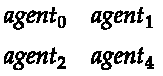
\includegraphics[width=0.4\linewidth]{figures/evo_1.pdf}
        \caption{All agents are initially unmerged.}
    \end{subfigure}%
    ~
    \begin{subfigure}[t]{0.3\textwidth}
        \centering
        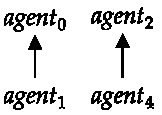
\includegraphics[width=0.4\linewidth]{figures/evo_2.pdf}
        \caption{$agent_0$ and $agent_1$ merge, $agent_2$ and $agent_3$ merge.}
    \end{subfigure}%
    ~
    \begin{subfigure}[t]{0.3\textwidth}
        \centering
        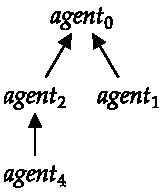
\includegraphics[width=0.4\linewidth]{figures/evo_3.pdf}
        \caption{$agent_0$ and $agent_2$ merge.}
    \end{subfigure}%

    \caption{Example of how coordinate frames are managed in Multi-Agent EVO. A path from $agent_m$ to $agent_n$ signifies that the agents are merged and there is an available translation from $agent_m$'s coordinate frame to $agent_n$'s.}
    \label{fig:evo-coord-frames}
\end{figure}

This method also allows us to retroactively transform trajectories into $agnet_0$'s coordinate from before the agents merged, allowing us to analyze the error of the pre-merge estimated relative trajectories.

\section{Simulation Environment}
\label{sec:simulation-environment}
The \nameref{sec:webots-simulator} section in the \nameref{sec:2} chapter explains the motivation behind using a simulator. Essentially, leveraging simulations enables much faster iterations and the ability to test my system in a variety of environments. This section will focus on the details of integrating the simulation software into my system.

Webots \autocite{Webots04} is an open-source 3D robotics simulator with realistic rendering, which is essential for testing a visual SLAM system. Unfortunately, Webots can not be built for the ARM Ubuntu VM I used for development, therefore it had to be run on MacOS, with data being streamed to the Ubuntu VM through a websocket bridge developed by Webots.

I have developed a ROS node that exposes the Webots camera and agent controls as ROS topics, following the abstract robot interface specifications. This allows my SLAM system to process the camera streams, and the motion controller / central management interface to control the agent's velocity in the simulated environment.

\begin{figure}[h]
    \centering
    \captionsetup{format=plain}
    \begin{minipage}[t]{0.575\linewidth}
        \centering
        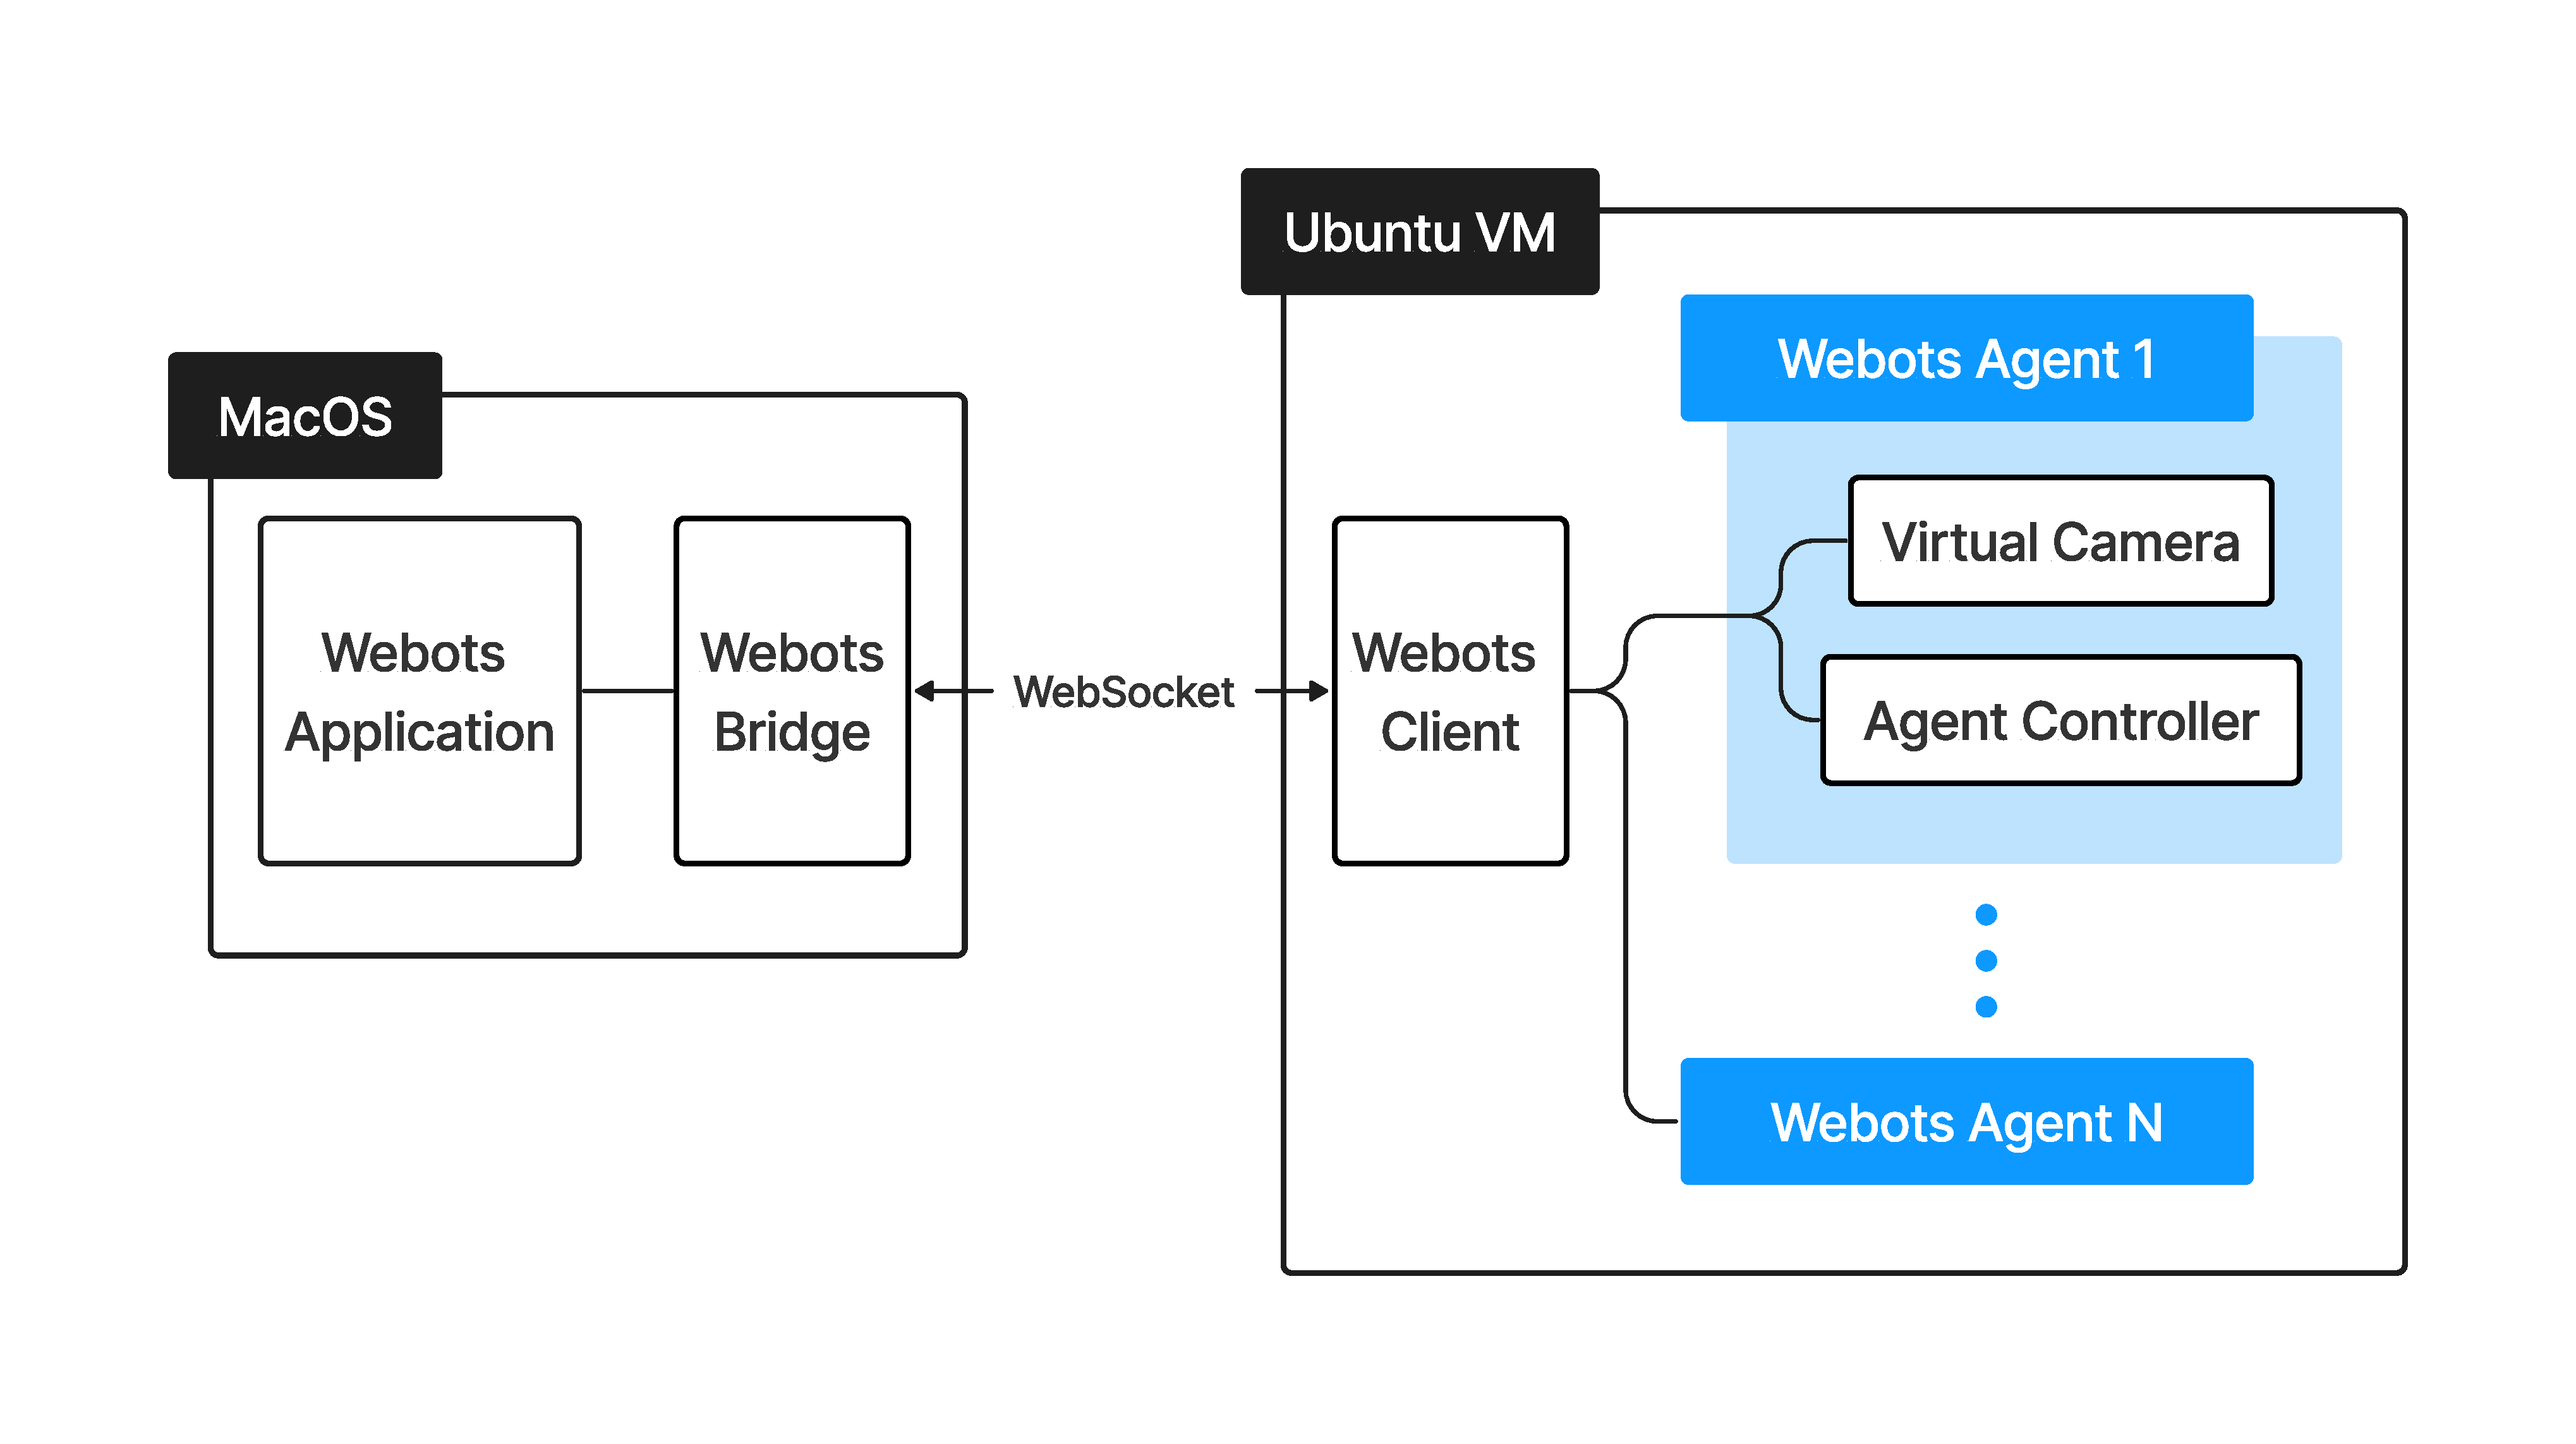
\includegraphics[trim=5cm 4.5cm 5cm 5cm, width=\linewidth]{figures/simulation_environment.pdf}

        \caption{Simulation system architecture. The Webots application runs on MacOS and is exposed to the Ubuntu VM as ROS topics by the custom \texttt{Webots Client} ROS node.}
        \label{fig:simulation-environment}
    \end{minipage}\hfill%
    ~
    \begin{minipage}[t]{0.4\linewidth}
        \centering
        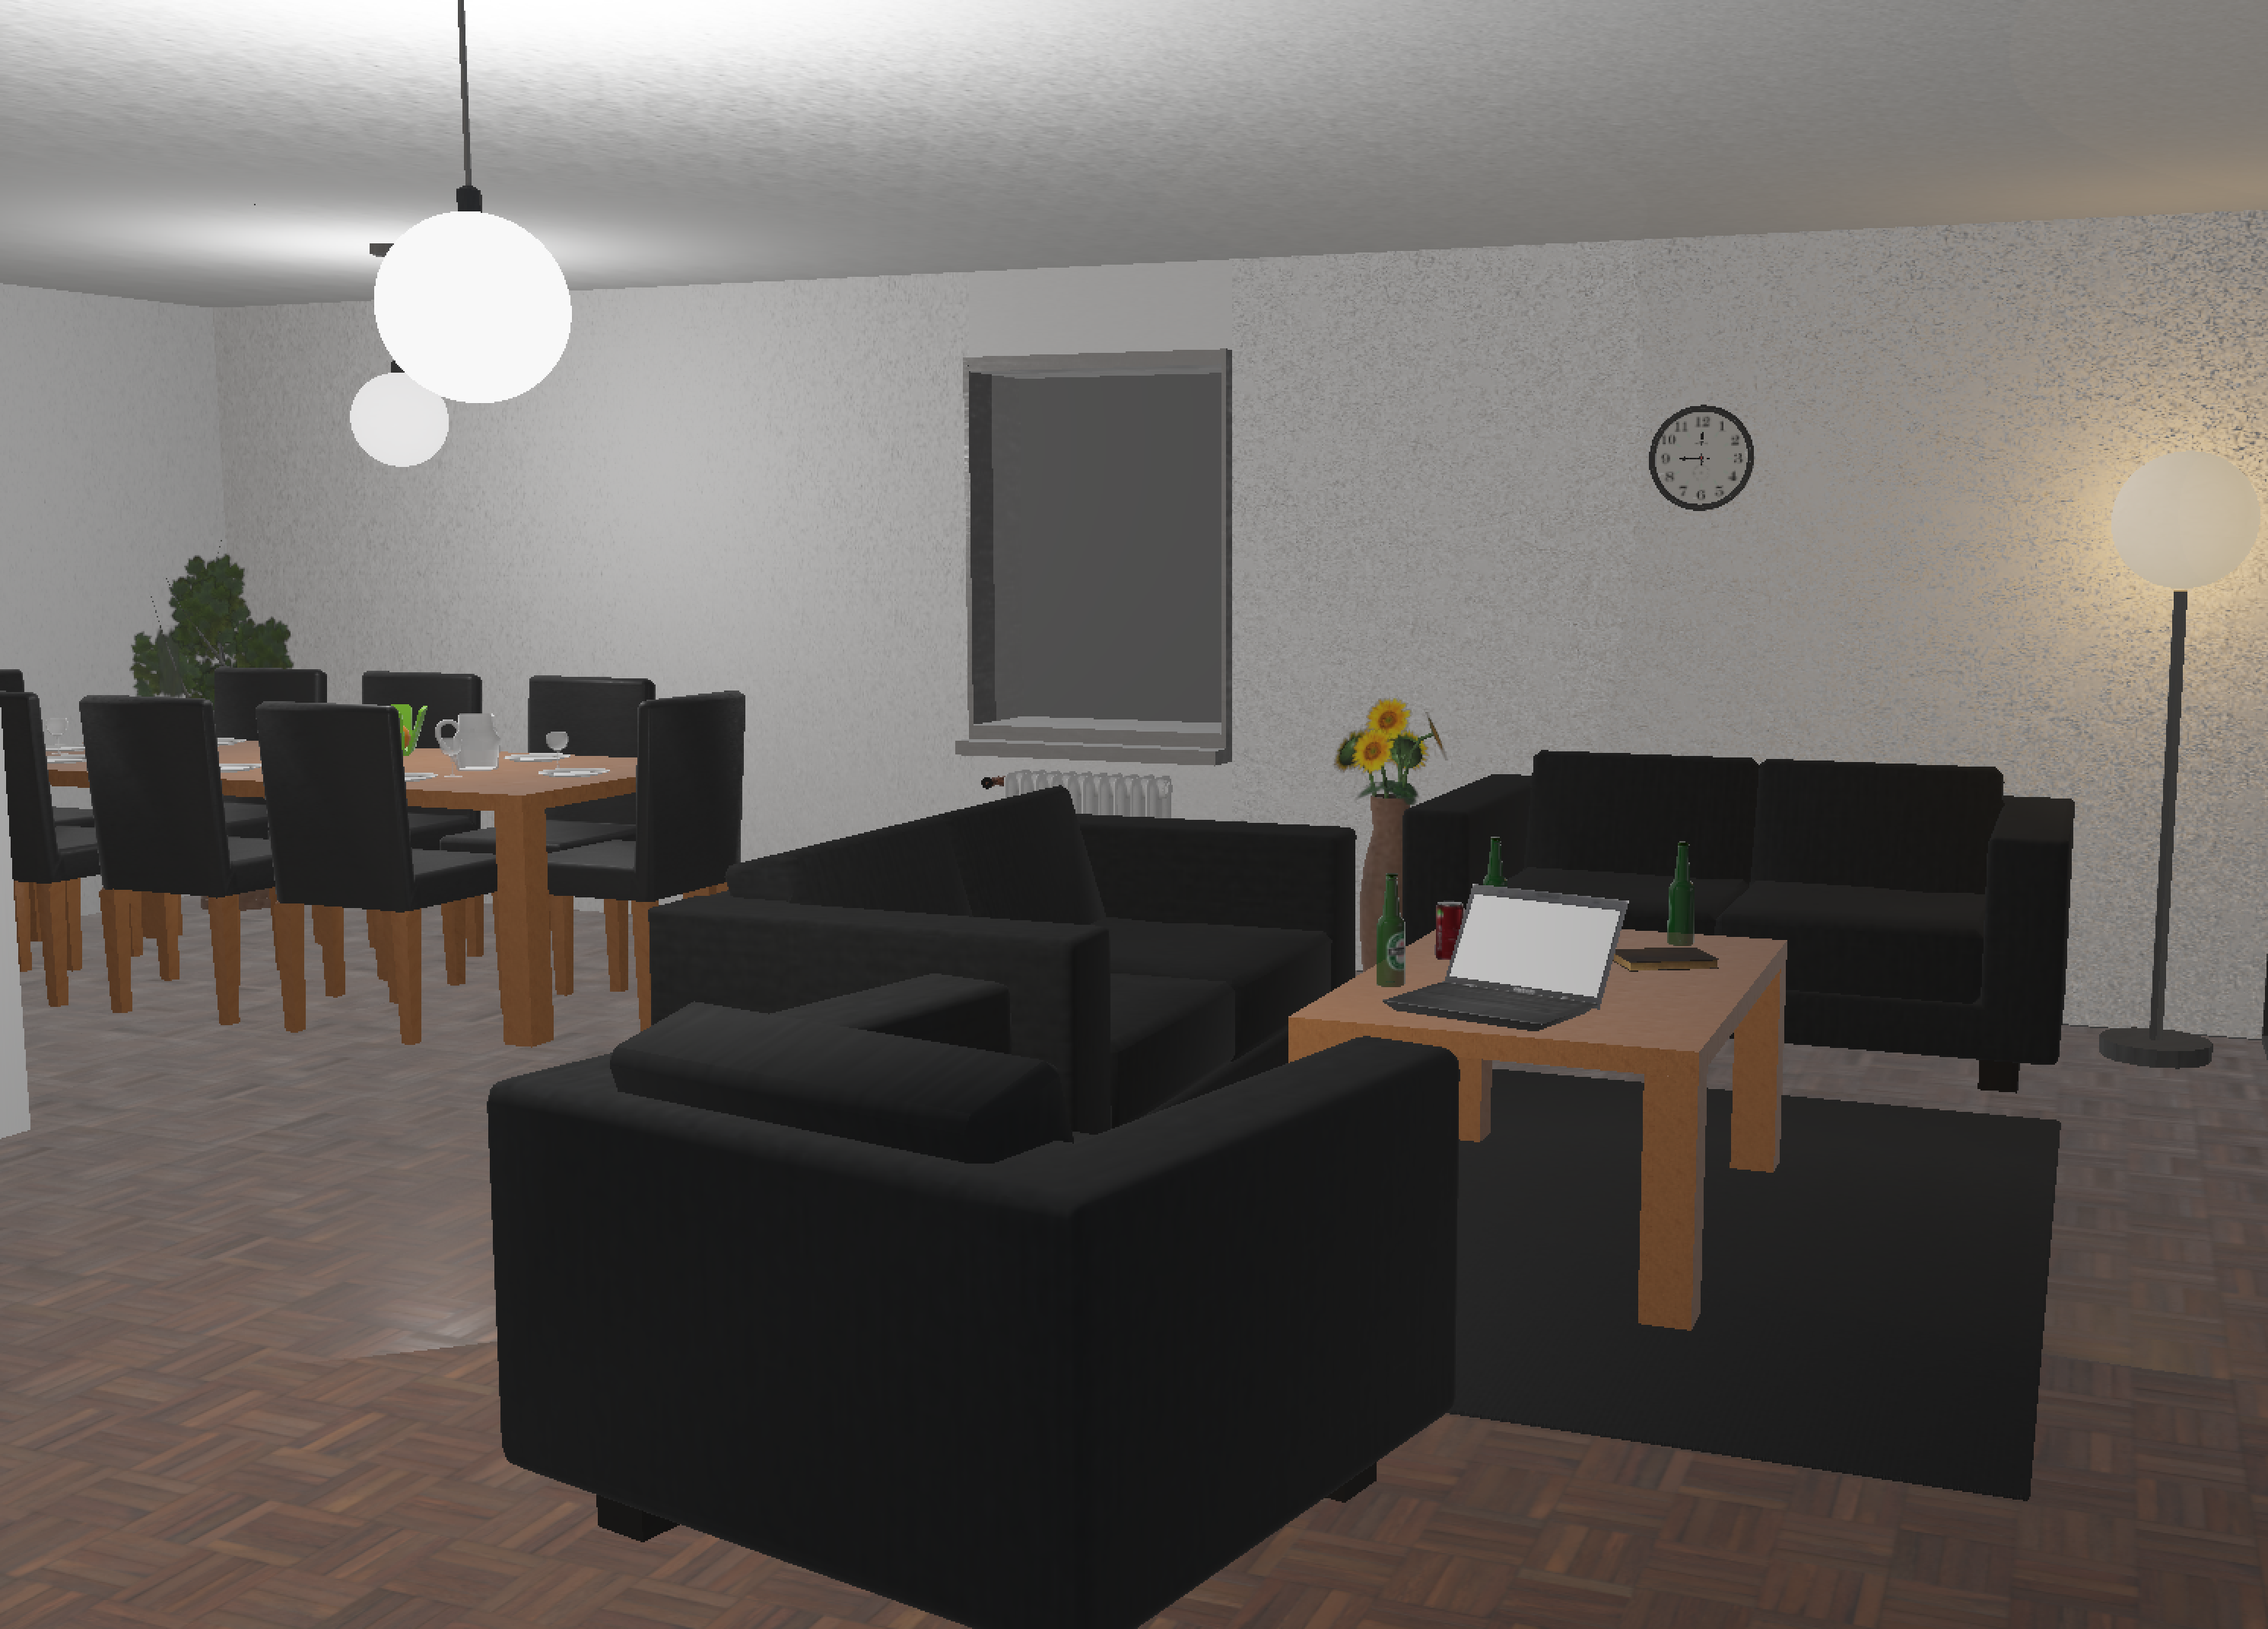
\includegraphics[width=\linewidth]{figures/webots_render.png}
        \caption{Webots render of the ``Apartment'' environment.}
    \end{minipage}
\end{figure}


\section{Real World Implementation}
\label{sec:real-world-implementation}
After months of development within a simulator, my distributed SLAM system was able to seamlessly be deployed to a real-world multi-agent system. This was largely due to the decisions made during the preparation phase. For example, the choice to use ROS as a communication middleware allows the agents to easily communicate, even when deployed on different physical devices. Another key choice was to abstract the implementation of nodes away behind the communication layer, as it allowed my system to interface with the physical robots without needing to make any changes to the SLAM system or motion controller nodes.

\subsection{Cambridge RoboMaster Platform}
\label{sec:cambridge-robomaster-platform}
I chose to deploy my system on the Cambridge RoboMaster, which is an omnidirectional robot platform with a NVidia Jetson Orin for compute (\autoref{fig:robomaster}). The only sensor used on the RoboMaster was the integrated Raspberry Pi HQ Camera, which provides a 1920x1080 image at 15hz. This was an obvious platform to use as ROS drivers for the camera and wheels had already been developed and a ground-based platform allows for easier testing.

As explained in the \nameref{sec:cicd} section, my system is compiled in the cloud and deployed on the robots in Docker containers.

As an aside, \textbf{I was an author of the paper \textit{The Cambridge RoboMaster: An Agile Multi-Robot Research Platform} \autocite{blumenkamp2024cambridge}}, which has been submitted to the 17th International Symposium on Distributed Autonomous Robotic Systems. My distributed SLAM system was included in the paper, with my system being run in conjunction with my multi-agent collision avoidance motion controller to evaluate the robotics platform's performance and capabilities.

% \subsection{Deploying with Docker}
% \label{sec:deploying-with-docker}
% My SLAM system is deployed on the RoboMasters in Docker containers. This allows my code to be compartmentalized from other projects being developed on the RoboMasters, as they are actively used by numerous researchers in the Prorok Lab. Additionally, I have set up a continuous integration process on GitHub to cross-compile a Docker container for the RoboMasters on every code push, which can then be pulled to the RoboMasters. This is a very useful feature, as building my full codebase can take upwards of 20 minutes on the NVidia Jetson Orins.

\subsection{OptiTrack Motion Capture System}
\label{sec:optitrack-motion-capture-system}
The ground truth for my real-world experiments is provided by the Prorok Lab's OptiTrack Motion Capture System, which advertises accuracies of $\leq$0.3mm at rates of 180hz \autocite{OptiTrackForRobotics}. The motion capture system publishes the real-time poses of the tracked objects to a ROS topic which can be recorded for later analysis.

\subsection{Raspberry Pi Video Publisher}
\label{sec:raspberry-pi-video-publisher}
This dissertation also presents the Raspberry Pi Video Publisher, an independent piece of infrastructure which I have developed both the hardware and software for. This platform publishes real-time camera data to a ROS topic and can be tracked by the lab's motion capture system. The two primary use cases for this platform are (1) dataset generation and (2) real-time AR visualization of 3D data (\autoref{sec:augmented-reality-visualization}).

The hardware for this platform consists of a Raspberry Pi 4b, Raspberry Pi Camera v2, 3D printed frame, and motion capture markers. The 3D-printed frame securely mounts the components together, allowing the system to be carried around or mounted to a tripod as shown in \autoref{fig:rpi-cam}.

ROS does not support streaming videos across a network, instead requiring frames to be sent as individual compressed images. This results in significant computational overhead, with a naive ROS video publisher implementation only being able to stream at 10 frames per second on the Raspberry Pi. To enable a 30-frame-per-second video stream, my implementation uses three threads. The first thread captures images from the camera, the second encodes them as a JPEG image, and the third publishes the images to a ROS topic.

As explained in the \nameref{sec:cicd} section, the software for this platform is entirely dockerized and a CI/CD pipeline has been implemented to automatically build and deploy the software to all Raspberry Pi video publishers when new code is pushed to the GitHub repository. The ease of use of the Raspberry Pi ROS video publisher platform has made them an invaluable tool and resolves the time-syncing issues previously faced when using the existing cameras in the Prorok Lab.

% As explained in the \nameref{sec:cicd} section, the software for this platform is entirely dockerized and a CI/CD pipeline has been implemented to automatically build and deploy the software to all Raspberry Pi video publishers when new code is pushed to the GitHub repository. This is particularly useful, as it is designed as a plug-and-play system that starts streaming video data as soon as it is turned on.

\begin{figure}[h]
    \centering
    \captionsetup{format=plain}
    \begin{minipage}[t]{0.475\linewidth}
        \centering
        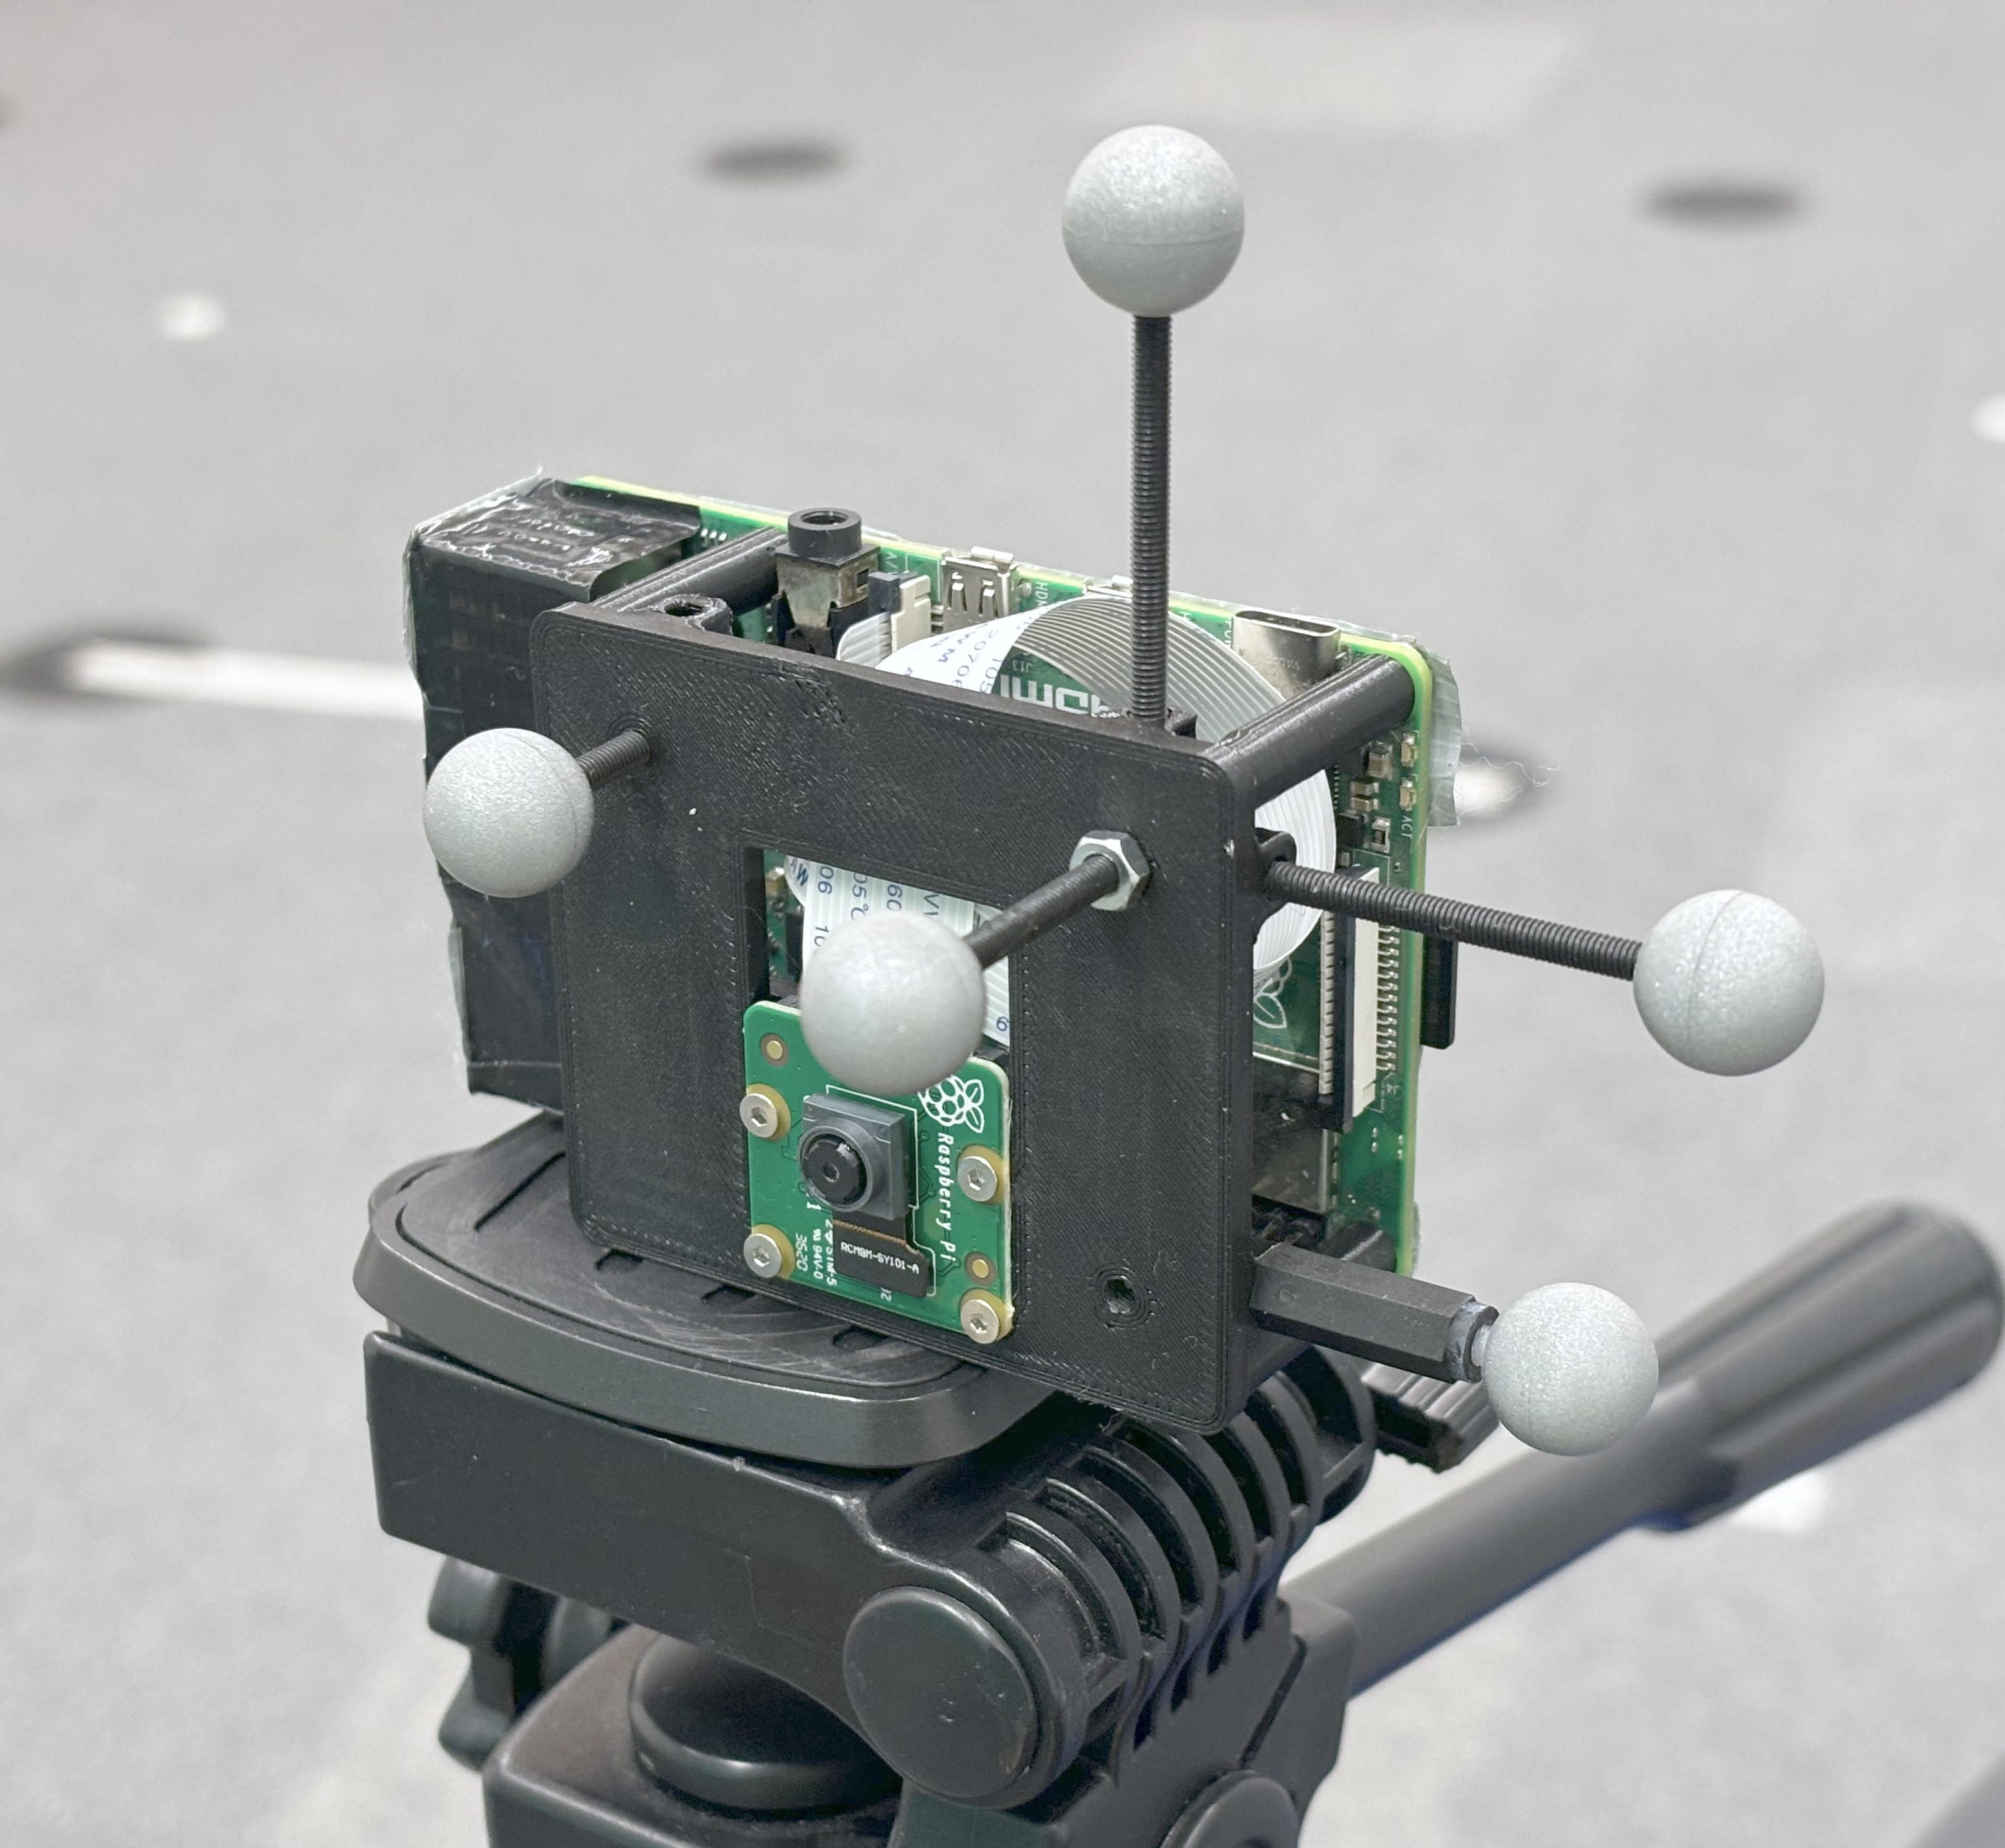
\includegraphics[height=2.5in]{figures/rpi_cam.jpg}

        \caption{Custom-built Raspberry Pi Video Publisher mounted on a tripod.}
        \label{fig:rpi-cam}
    \end{minipage}\hfill%
    ~
    \begin{minipage}[t]{0.475\linewidth}
        \centering
        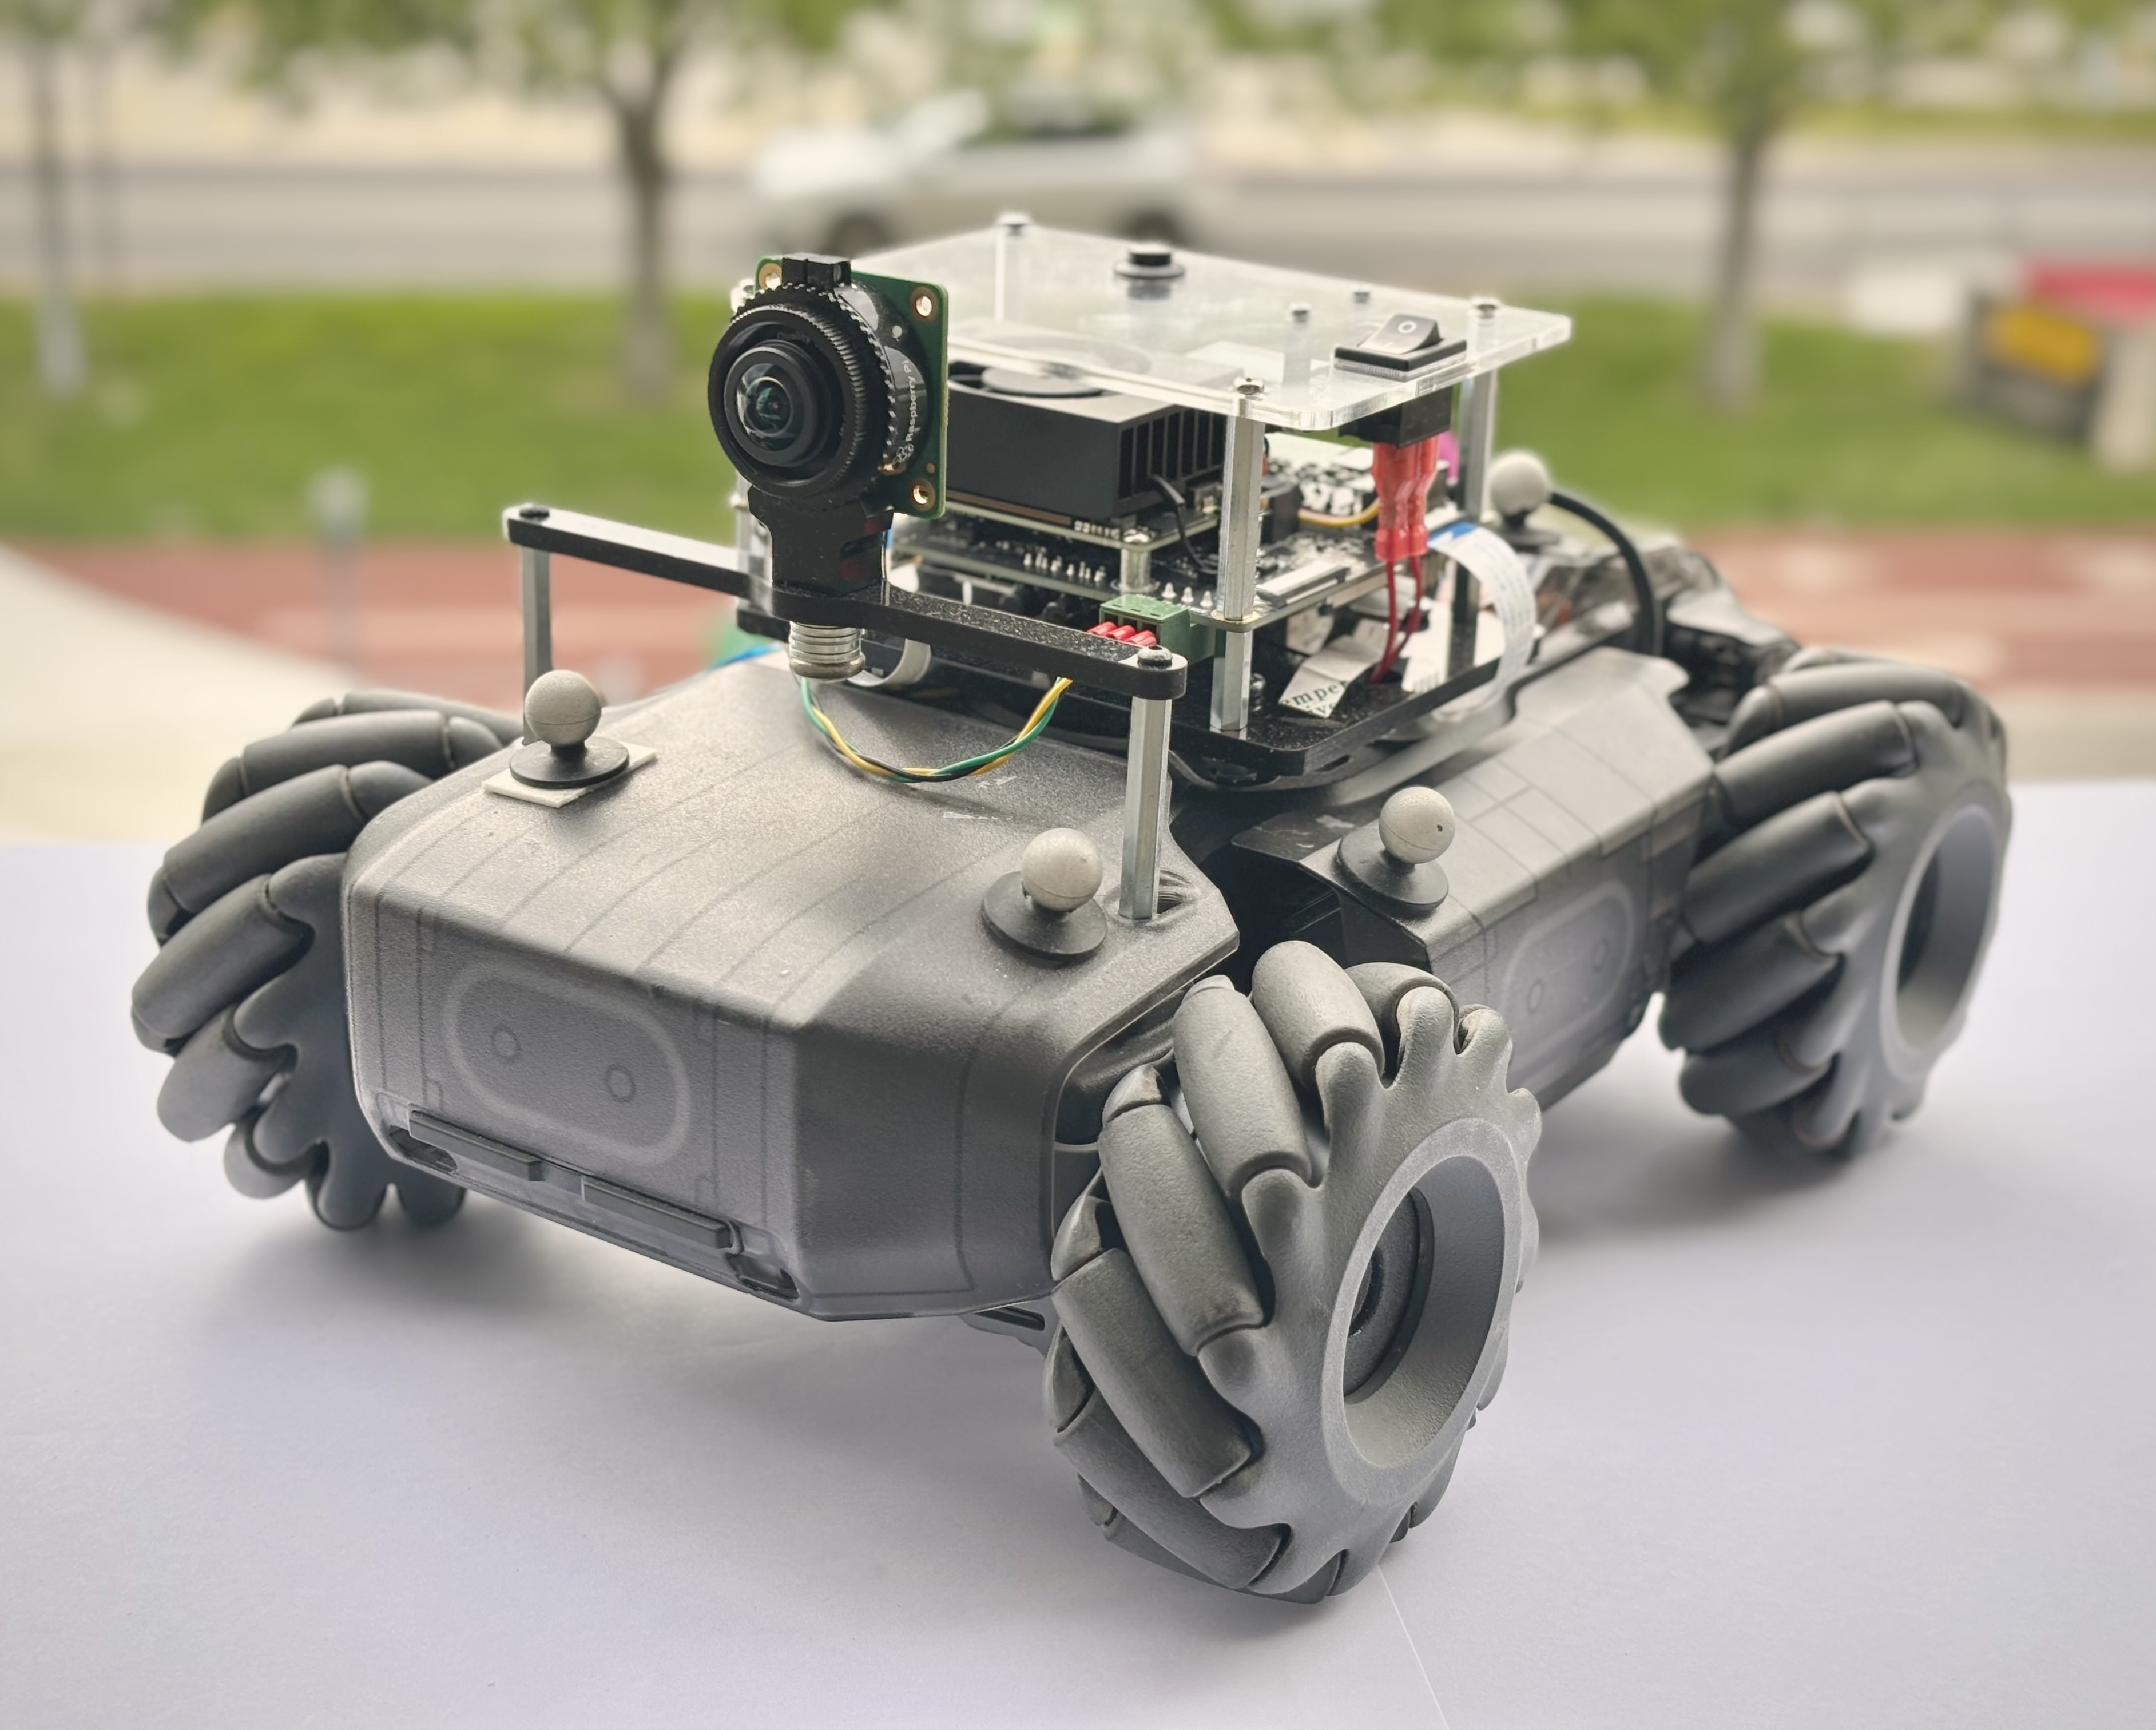
\includegraphics[height=2.5in]{figures/robomaster.jpg}
        \caption{Cambridge RoboMaster platform with NVidia Jetson Orin and Raspberry Pi HQ Camera.}
        \label{fig:robomaster}
    \end{minipage}
\end{figure}


\subsection{Augmented Reality Visualization}
\label{sec:augmented-reality-visualization}
The Raspberry Pi Video Publisher platform is tracked by the motion capture system, allowing us to project 3D visualization data onto the captured video. This can be used to visualize the SLAM system's keyframe and map point locations in the real world and to view how the predicted trajectory aligns with reality.

To overlay this data on the video, we must first align the SLAM system and motion capture systems' coordinate frames. This needs to be done on every run, as monocular SLAM systems have an arbitrary scale. Therefore, we use the \nameref{sec:kabsch-umeyama-algorithm} to align the trajectories captured by the motion capture system and SLAM system after enough data has been collected to create a successful alignment. We can then use Foxglove Studio to draw our 3D markers and project them on top of the tracked camera's video stream, a snapshot of which is displayed in \autoref{fig:ar-overlay-map-points}.

Importantly, the tool is built around the standard ROS marker interface. This makes it a generic platform that can give an AR visualization of any experiment being conducted in a motion capture environment.

To my knowledge, this system is the first of its kind to be used in such a project. Not only is it visually impressive, but it also can be used for further analysis and understanding. For example, this visualization helped me identify that my collision avoidance demo was being severely impacted by latency spikes which I proceeded to fix.

\begin{figure}[h]
    \centering
    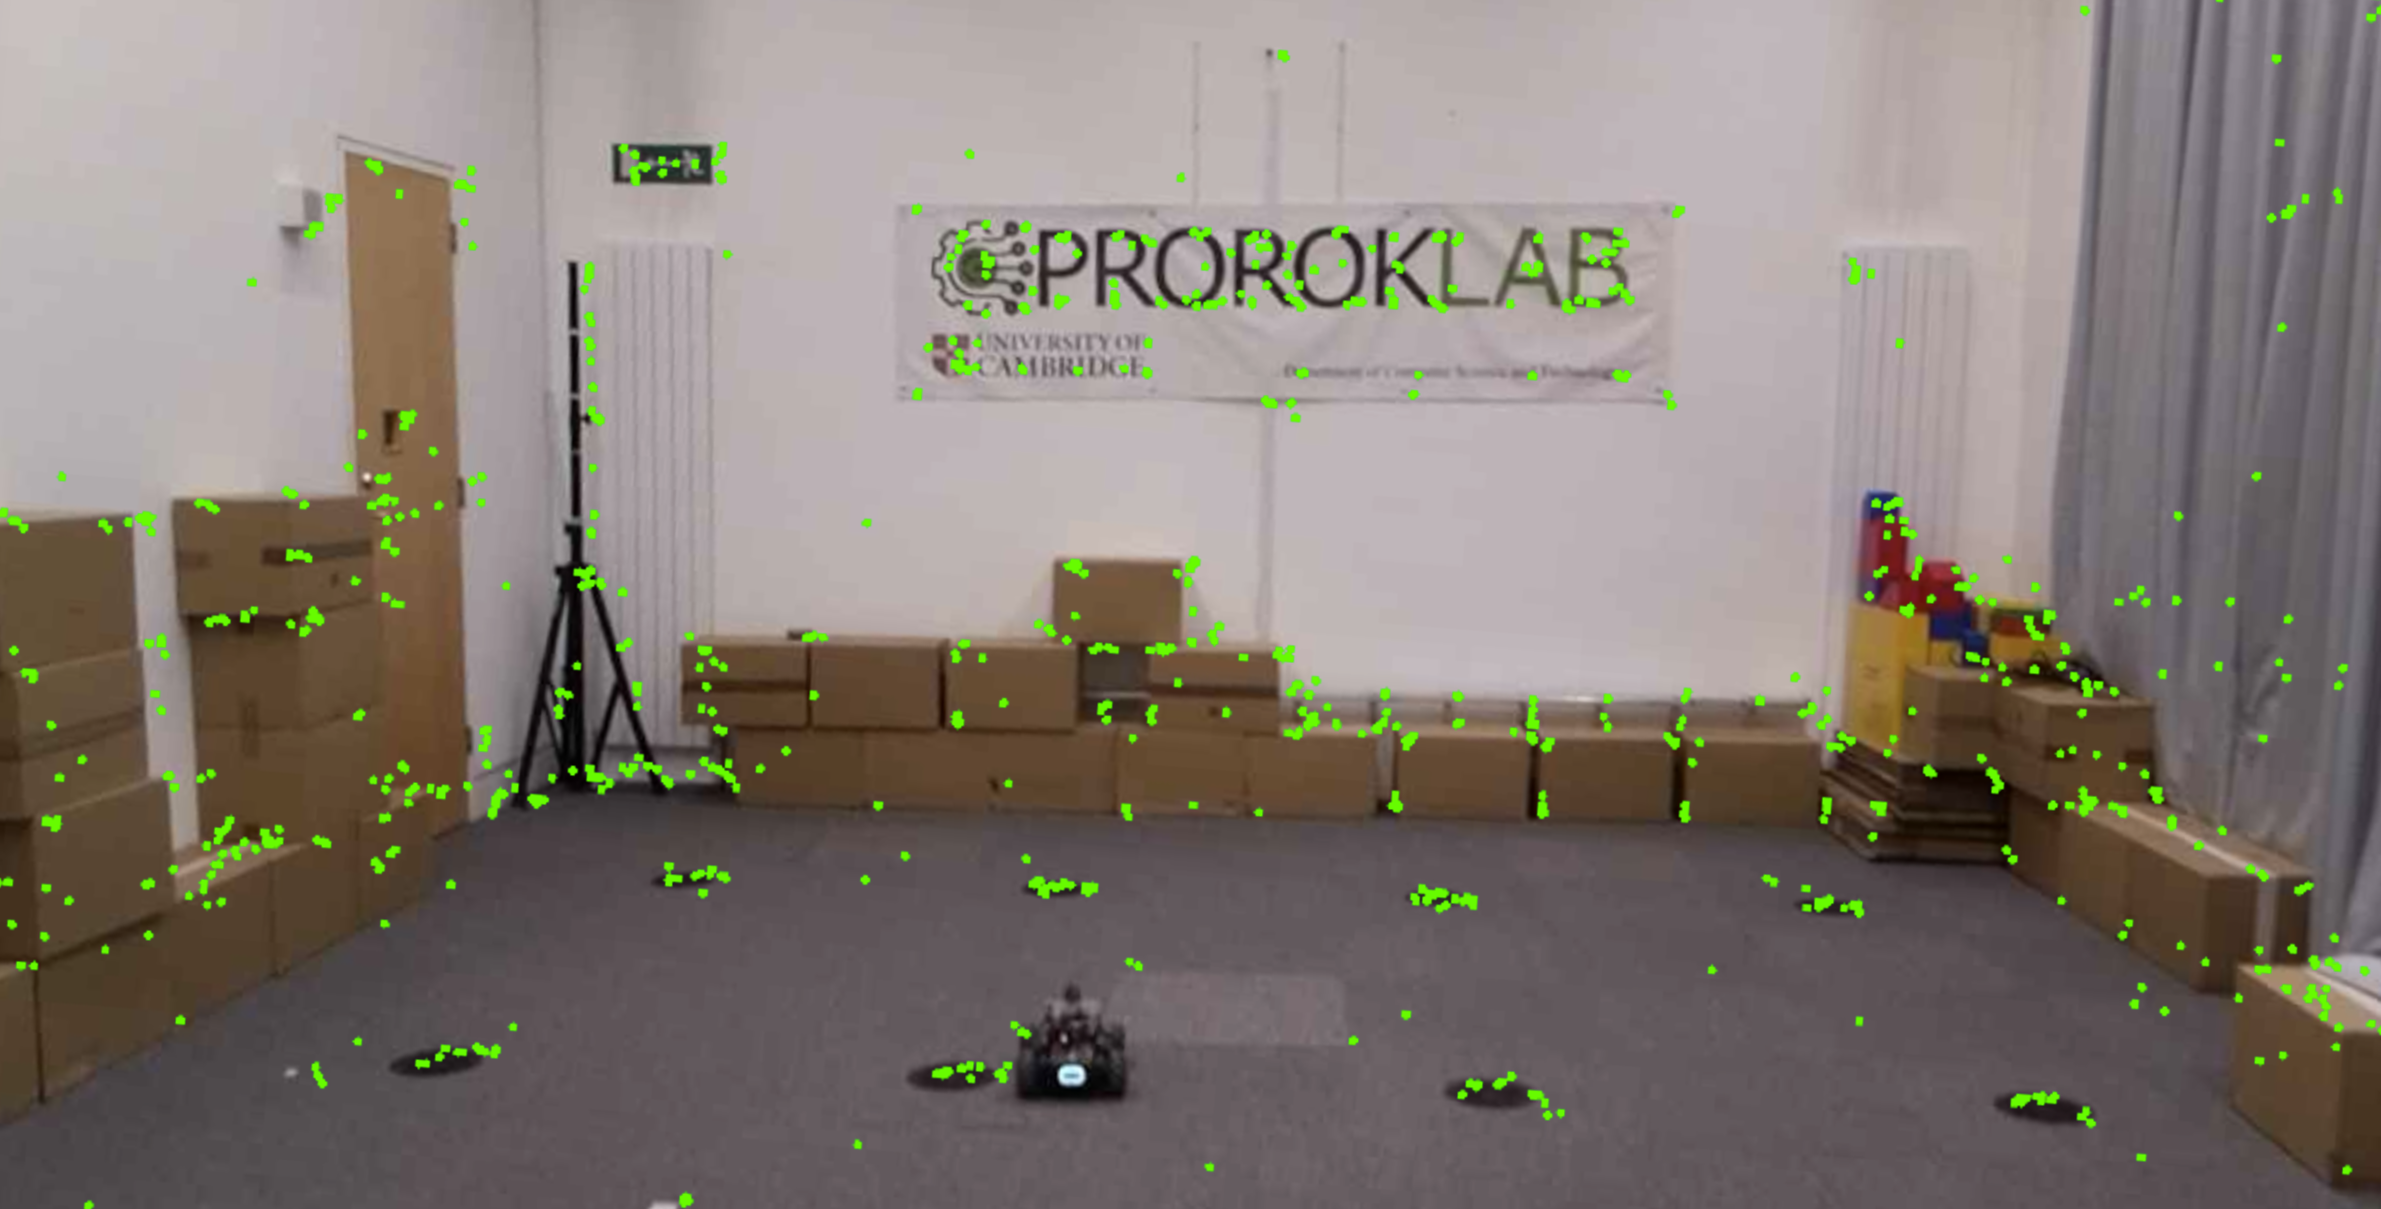
\includegraphics[width=0.8\linewidth]{figures/ar_overlay_map_points.png}

    \caption{Features tracked by the RoboMaster overlayed over an ``external perspective" handheld video from my Raspberry Pi Video Publisher. This visualization makes it clear that my SLAM system is tracking the corners of boxes, letters on the Prorok Lab banner, and the floor vents. \captionbreak Note that the features are generated by the RoboMaster, and then reprojected onto the video captured by the Raspberry Pi as it moves through space. This is made clear in the video demonstration of this feature at 2m25s of the supplementary video\protect\footnotemark[1].}
    \label{fig:ar-overlay-map-points}
\end{figure}
\footnotetext[1]{Supplementary video URL: \url{https://cam-diss.s3.amazonaws.com/video.mp4}}

\newpage
\section{Repository Overview}
\label{sec:repository-overview}

\newcommand{\locindent}{3.3em}
\newcommand{\locsmallindent}{2em}
\newcommand{\locdiff}[3]{
    \makebox[#3][r]{\textcolor{PineGreen}{\texttt{+#1}}}
    \makebox[#3][r]{\textcolor{BrickRed}{\texttt{-#2}}}
}
\newcommand{\locadd}[2]{
    \makebox[#2][r]{\textcolor{PineGreen}{\texttt{+#1}}}
    \makebox[#2][r]{}
}
\newcommand{\locaddnospace}[2]{
    \makebox[#2][r]{\textcolor{PineGreen}{\texttt{+#1}}}
}
\newcommand{\locdoublespace}[1]{
    \makebox[#1][r]{}
    \makebox[#1][r]{}
}
\newcommand{\locsinglespace}[1]{
    \makebox[#1][r]{}
}

My dissertation consists of five ROS packages, a Python library, 3D designs, and dozens more miscellaneous files, amounting to \textbf{35,000\texttt{+} lines of code} across \textbf{108 files} and \textbf{three repositories}. While lines of code and number of files are a poor measurement of complexity, I still hope to illustrate the scale of this software engineering project. The following section gives a brief overview of my codebase's structure.

The \texttt{distributed\_visual\_slam} repository (\autoref{fig:repo-overview-main}) contains the core SLAM system and all the infrastructure needed to run it. This includes five ROS packages: \texttt{slam\_system}, \texttt{motion\_controller}, \texttt{webots\_sim}, \texttt{central\_management\_interface}, and \texttt{interfaces}, which all follow the standard ROS package structure. \texttt{slam\_system} and \texttt{interfaces} are written in C++ and built using CMake, while the remaining packages are Python-based.

\begin{figure}[h]
    \centering
    \captionsetup{skip=0.5em}
    \begin{minipage}[t]{\linewidth}
        \footnotesize
        \setlength{\DTbaselineskip}{12pt}
        \dirtree{%
            .1 distributed\_visual\_slam/\DTcomment{\locdiff{5,953}{1,598}{\locindent}}.
            .2 src/.
            .3 slam\_system/\DTcomment{Core SLAM package (\cref{sec:slam-system})\locdiff{3,303}{1,598}{\locindent}}.
            .5 include/\DTcomment{Decentralized system manager headers\locaddnospace{242}{\locindent}}.
            .5 src/\DTcomment{Decentralized system manager (\cref{sec:decentralized-system-manager})\locaddnospace{1,283}{\locindent}}.
            .5 orb\_slam3/\DTcomment{Modified ORB-SLAM3 codebase\locdiff{1,728}{1,598}{\locindent}}.
            .5 configs/\DTcomment{Config for different camera systems\locsinglespace{\locindent}}.
            .5 ....
            .4 ....
            .3 motion\_controller/\DTcomment{Motion controller package (\cref{sec:motion-controller})\locaddnospace{600}{\locindent}}.
            .4 motion\_controller/.
            .5 collision\_avoidance.py\DTcomment{(\cref{sec:multi-agent-collision-avoidance-implementation})\locaddnospace{142}{\locindent}}.
            .5 follow\_the\_leader.py\DTcomment{(\cref{sec:follow-the-leader})\locaddnospace{78}{\locindent}}.
            .5 helpers/\DTcomment{\locaddnospace{310}{\locindent}}.
            .4 ....
            .3 webots\_sim/\DTcomment{Simulation package (\cref{sec:simulation-environment})\locaddnospace{288}{\locindent}}.
            .4 webots\_sim/robot\_driver.py\DTcomment{\locaddnospace{58}{\locindent}}.
            .4 launch/robot\_launch.py\DTcomment{\locaddnospace{42}{\locindent}}.
            .4 worlds/.
            .4 ....
            .3 central\_management\_interface/\DTcomment{Centeral management interface package (\cref{sec:central-management-interface})\locaddnospace{442}{\locindent}}.
            .3 evaluation/\DTcomment{Jupyter Notebooks for evaluation\locaddnospace{1033}{\locindent}}.
            .3 interfaces/\DTcomment{Custom ROS message type definitions\locaddnospace{109}{\locindent}}.
            .3 tools/\DTcomment{Misc. scripts\locaddnospace{42}{\locindent}}.
            .2 .github/workflows/config.yml\DTcomment{CI/CD configuration (\cref{sec:cicd})\locaddnospace{73}{\locindent}}.
            .2 Dockerfile\DTcomment{Main dockerfile for the project (\cref{sec:cicd})\locaddnospace{20}{\locindent}}.
            .2 nvidia\_jetson.Dockerfile\DTcomment{Dockerfile for the NVidia Jetson (\cref{sec:cicd})\locaddnospace{30}{\locindent}}.
            .2 ....
        }
    \end{minipage}
    \caption{Repository overview for my distributed visual SLAM system. Line count does not include non-code files (e.g. camera configurations, simulation worlds, et cetera.) \captionbreak \texttt{git diff} is used for the \texttt{orb\_slam3} folder, as it is a fork of an existing single-agent SLAM system \autocite{ORBSLAM3_TRO}. The \texttt{git diff} excludes reformatting and the mass deletion of unused files.}
    \label{fig:repo-overview-main}
\end{figure}

The \texttt{rpi\_ros2\_camera\_publisher} repository (\autoref{fig:repo-overview-rpi-video}) holds the code, 3D files, and CI/CD configuration for the Raspberry Pi Camera Publisher system. The provided Systemctl service file configures the Raspberry Pi to pull and run the latest docker image on startup.

\begin{figure}[h]
    \centering
    \captionsetup{justification=raggedright,singlelinecheck=false, skip=0.5em}
    \begin{minipage}[t]{\linewidth}
        \footnotesize
        \setlength{\DTbaselineskip}{12pt}
        \dirtree{%
            .1 rpi\_ros2\_camera\_publisher/\DTcomment{(\cref{sec:raspberry-pi-video-publisher})\locaddnospace{190}{\locsmallindent}}.
            .2 src/.
            .3 send\_images.py\DTcomment{\locaddnospace{132}{\locsmallindent}}.
            .2 .github/workflows/config.yml\DTcomment{CI/CD configuration (\cref{sec:cicd})\locaddnospace{36}{\locsmallindent}}.
            .2 3D\_files/.
            .2 Dockerfile\DTcomment{Main dockerfile for the project (\cref{sec:cicd})\locaddnospace{10}{\locsmallindent}}.
            .2 docker-rpi-cam.service\DTcomment{Systemctl service file\locaddnospace{11}{\locsmallindent}}.
            .2 ....
        }
    \end{minipage}
    \caption{Repository overview for the Raspberry Pi Camera Publisher system.}
    \label{fig:repo-overview-rpi-video}
\end{figure}

The \texttt{multi\_agent\_evo} repository (\autoref{fig:repo-overview-multi-agent-evo}) is a modified version of the EVO library \autocite{grupp2017evo} that supports the evaluation of multi-agent SLAM systems.

\begin{figure}[h]
    \centering
    \captionsetup{skip=0.5em}
    \begin{minipage}[t]{\linewidth}
        \footnotesize
        \setlength{\DTbaselineskip}{12pt}
        \dirtree{%
            .1 multi\_agent\_evo/\DTcomment{(\cref{sec:multi-agent-evo})\locdiff{399}{54}{\locsmallindent}}.
            .2 evo/.
            .3 core/\DTcomment{\locdiff{125}{5}{\locsmallindent}}.
            .4 trajectory.py\DTcomment{Class for operating on trajectories\locdiff{115}{4}{\locsmallindent}}.
            .4 ....
            .3 tools/\DTcomment{\locdiff{272}{49}{\locsmallindent}}.
            .4 coordinate\_frame\_decoder.py\DTcomment{Parse multi-agent coordinate frame data\locadd{202}{\locsmallindent}}.
            .4 ....
            .2 ....
        }
    \end{minipage}
    \caption{Repository overview for the Multi-Agent EVO evaluation library. \captionbreak Note that a \texttt{git diff} is given for the repository, as it is a fork of the single agent evaluation library EVO \autocite{grupp2017evo}.}
    \label{fig:repo-overview-multi-agent-evo}
\end{figure}

